\documentclass[a4paper,12pt, final]{report}


% Paquetes necesarios para la portada
\usepackage[spanish]{babel}
\usepackage{background}
\usepackage{textpos}
\usepackage{graphicx}
\usepackage{float}
\usepackage{multirow}
\usepackage[table]{xcolor}
\usepackage{makecell} 
\usepackage{array}


\usepackage[
backend=biber,
style=apa,
sortcites,
url=true]{biblatex}
\addbibresource{references.bib} 
\usepackage[colorlinks=true, citecolor=blue,linkcolor=black, urlcolor=blue]{hyperref}


\begin{document}
	
	% Incluir la portada
	\backgroundsetup{
	scale=1,
	color=black,
	opacity=1,
	angle=0,
	contents={%
		
\includegraphics[width=19cm,height=28.5cm]{doc_images/background.png}
	}% 
}

\begin{titlepage}
	\BgThispage  % Aplica el fondo solo a esta página (portada)
	
	\begin{textblock}{3.5}[0.5,0.5](0.5,0.5)
		
\includegraphics[width=\linewidth]{doc_images/logoUTDT.png}\\[3.5cm]  % Ajusta la imagen si es necesario
	\end{textblock}
	
	\begin{center}
		{Universidad Torcuato Di Tella\\[0.2cm]
			\textbf{Master in Management + Analytics}\\[0.2cm]
			\vspace{2cm}
			{\large \textbf{Tesis de Maestría}}\\[0.6cm]
			
			% Title
			\rule{\linewidth}{0.5mm} \\[0.1cm]
			{ \huge \bfseries Aplicación de IA en el Control de Calidad de Imágenes Retinales para Diagnóstico de Retinopatía Diabética
				\\[0.1cm] }
			\rule{\linewidth}{0.5mm} \\[1.5cm]
			
			% Autores y tutor
			\noindent
			
			{\Large  \emph{Alumna:}}\\[0.3cm]
			{\large  
				Gabriela Moran \\[0.2cm]
				\\[1cm]
				
				{\Large  \emph{Tutor:}}\\[0.3cm]
				{\large  Santiago Cisco}
				
				\vspace{3cm}
				% Parte inferior de la página
				{Mayo 2025}
			\end{center}
		\end{titlepage}
\backgroundsetup{contents={}}
	
	\chapter*{Resumen}
\addcontentsline{toc}{chapter}{Resumen}

\par Esta tesis aborda el problema de evaluar automáticamente la calidad adecuada para la interpretación clínica de imágenes retinianas. Se propone y compara el desempeño de dos enfoques: un modelo convolucional entrenado específicamente (ResNet-18 fine-tuned) y un modelo multimodal de propósito general (GPT-4o), evaluado en modalidades \textit{zero-shot} y \textit{few-shot}. Los resultados muestran que el modelo entrenado obtuvo mejores métricas de precisión y estabilidad, mientras que GPT-4o alcanzó valores elevados de recall, pero con una alta tasa de falsos positivos. Aunque los modelos multimodales requieren poco esfuerzo de implementación inicial, su rendimiento está fuertemente condicionado por el diseño del prompt y la selección de ejemplos, lo que reintroduce un grado de intervención por parte del investigador. Además, al tratarse de modelos ofrecidos como servicio, se identifican limitaciones en cuanto a reproducibilidad, trazabilidad y control. Se concluye que, si bien GPT-4o aún no tiene la robustez necesaria para ser utilizado de forma autónoma en tareas clínicas sensibles, podría integrarse como herramienta auxiliar en entornos híbridos de diagnóstico, especialmente en escenarios con barreras de acceso a la atención.

\vspace{1em}
\noindent
\textbf{Palabras clave:} Retinopatía diabética, control de calidad de imágenes, \\
clasificación de imágenes médicas, modelos multimodales, GPT-4o, aprendizaje \textit{zero-shot}.

	\chapter*{Abstract}
\addcontentsline{toc}{chapter}{Abstract}

\par This thesis addresses the problem of automatically assessing whether retinal images meet the quality requirements for clinical interpretation. It proposes and compares the performance of two approaches: a specifically trained convolutional model (ResNet-18 fine-tuned) and a general-purpose multimodal model (GPT-4o), evaluated under \textit{zero-shot} and \textit{few-shot} settings. Results show that the trained model achieved better precision and stability metrics, while GPT-4o reached high recall values but with a high rate of false positives. Although multimodal models require minimal initial implementation effort, their performance is strongly influenced by prompt design and example selection, which reintroduces a degree of developer intervention. Furthermore, as models provided as a service, they present limitations in terms of reproducibility, traceability, and control. It is concluded that, although GPT-4o does not yet have the robustness required to be used autonomously in sensitive clinical tasks, it could serve as an auxiliary tool in hybrid diagnostic systems, particularly in contexts with limited access to care.


\vspace{1em}
\noindent
\textbf{Keywords:} Diabetic retinopathy, image quality assessment, \\
medical image classification, multimodal models, GPT-4o, zero-shot learning.

	
	% Tabla de Contenidos (Índice)
	\thispagestyle{empty}  % Sin número de página en esta página
	\newpage
	\tableofcontents  % Genera el índice
	\thispagestyle{empty}  % Sin número de página en el índice
	
	% Incluir la introducción
	\input{Introduction.tex}
	\chapter{Motivación}


\section{El desafío de prevenir la ceguera irreversible en personas con diabetes}
La diabetes es una enfermedad metabólica crónica caracterizada por altos niveles de azúcar en sangre, que con el tiempo puede causar daños graves en diversos órganos, como el corazón, los riñones, los ojos, así como en los vasos sanguíneos y los nervios \parencites{ops_diabetes}. En el mundo, más de 537 millones de adultos, entre 20 y 79 años, viven actualmente con diabetes. Se estima que esta cifra aumentará a 783 millones para 2045. Además, los gastos asociados con la enfermedad se han incrementado en un 316\% en los últimos 15 años, alcanzando al menos 966 mil millones de dólares \parencites{idf_2021}.


En Argentina, se registró un aumento significativo de la prevalencia de glucemia elevada/diabetes en la población total (18 años y más), pasando del 9,8\% en 2013 al 12,7\% en 2018. Además, el 19,8\% de la población presenta riesgo alto o muy alto de desarrollar diabetes mellitus en los próximos diez años  \parencites{indec2019}. 

Existen ciertas complicaciones oculares relacionadas con la diabetes, como la retinopatía diabética (RD), que se produce cuando los elevados niveles de glucosa dañan los vasos sanguíneos de la retina. Con el tiempo, los vasos sanguíneos dañados pueden perder líquido o sangrar provocando alteraciones en la vista. A nivel global, se estima que aproximadamente un tercio de las personas con diabetes desarrolla algún grado de RD, siendo esta la principal causa de ceguera en adultos en edad laboral \parencites{idf_2021} y la segunda causa de ceguera en Argentina (16\%) \parencites{silva2015}.

Al ser una enfermedad crónica, es fundamental instruir a la población sobre el autocuidado adecuado y el seguimiento de la enfermedad y sus complicaciones. Por ello, las guías recomiendan realizar anualmente una imagen de fondo de ojo \parencites{ops_diabetes, ops_clinica_diabetes}. La detección temprana, junto con el tratamiento oportuno y un seguimiento adecuado, puede reducir hasta en un 95\% el riesgo de pérdida de visión asociada con la RD \parencites{nei2023}.

En una zona rural de La Pampa, un estudio reveló que más del 30\% de las personas evaluadas nunca se había realizado un fondo de ojos. Además, el riesgo de desarrollar RD era significativamente mayor en quienes no se sometían a este examen desde hace más de cinco años, destacando la falta de adherencia a esta práctica esencial para la detección temprana \parencites{ortizbasso2022}.

En relación a la prevalencia de la RD en Argentina, la Campaña de Prevención de Ceguera por Diabetes, en el año 2023, identificó un 29.4\% de RD \parencites{oftalmologos2023}.


\section{Barreras en el diagnóstico temprano de la retinopatía diabética y sus consecuencias}
En Argentina, las desigualdades en el acceso al diagnóstico y tratamiento de la diabetes y sus complicaciones, como la retinopatía diabética, están marcadas por diferencias socioeconómicas y geográficas. Según la Encuesta Nacional de Factores de Riesgo, la prevalencia de diabetes por autorreporte varía considerablemente entre regiones: en la Ciudad de Buenos Aires es del 8,8\%, mientras que en la provincia de San Luis alcanza el 17,3\%, siendo esta la más alta del país.

El nivel educativo también juega un rol importante, ya que las personas con menor nivel educativo (hasta primario incompleto) tienen una prevalencia de diabetes de 22,9\%, en contraposición al 10,3\% de quienes alcanzaron el nivel secundario completo o superior. Estas diferencias reflejan la influencia del acceso a la información y los recursos preventivos.

En relación a los estudios para la detección temprana de complicaciones, las desigualdades también son evidentes. Las personas de sexo femenino reportan menos exámenes de fondo de ojo que el sexo masculino, y las personas que dependen exclusivamente del sistema público de salud realizan menos estudios de la vista en comparación con aquellas que cuentan con algún tipo de cobertura médica privada. Asimismo, el ingreso económico es un factor relevante: mientras que solo el 30,1\% de las personas en el quintil de ingresos más bajos realizó estudios de la vista, este porcentaje asciende al 47,8\% en el quintil más alto \parencites{indec2019}.

Por otro lado, en las zonas rurales de Argentina, las barreras para acceder al diagnóstico temprano se ven exacerbadas por la centralización del sistema de salud, que obliga a las personas a recorrer largas distancias a los centros de salud ya sea para un exámen o recibir el tratamiento correspondiente \parencites{ortizbasso2020}.

Cuando la RD se detecta en etapas tempranas, seguir una dieta saludable, controlar los niveles de azúcar en sangre y la presión arterial puede prevenir su progresión a formas más graves e incluso mejorar parcialmente la visión. Sin embargo, si la RD no se diagnostica hasta etapas más avanzadas, el tratamiento necesario es más complejo y costoso, e incluso puede requerir cirugía para reparar el daño en la retina. El diagnóstico temprano no solo mejora los resultados de salud, sino que también tiene un impacto económico positivo tanto para los pacientes como para el sistema de salud \parencites{aao2023}.


\section{Potencial de las soluciones basadas en inteligencia artificial}
En países de ingresos bajos y medios, el cribado de la RD se basa principalmente en la evaluación del fondo de ojo realizada por oftalmólogos. Sin embargo, este enfoque resulta ineficiente frente a las limitaciones de recursos humanos y las barreras de acceso al sistema de salud previamente discutidas \parencites{piyasena2018}.

Según \cite{ortizbasso2023}, diferentes regiones del mundo han incorporado programas de telemedicina para la detección precoz de RD, logrando mejoras significativas en el acceso al sistema de salud, optimización de recursos y control de la enfermedad. Programas implementados en Inglaterra, Estados Unidos e India, han demostrado su efectividad para incrementar la cobertura y reducir complicaciones derivadas de la RD. En el contexto local, el estudio destaca que, tras la implementación de un programa de teleoftalmología en una zona rural de la provincia de La Pampa, la tasa anual de exámenes de fondo de ojos realizados en personas con diabetes aumentó significativamente, mostrando el potencial impacto positivo de estas iniciativas en áreas con recursos limitados.

Los avances en inteligencia artificial (IA) y, en particular, en aprendizaje profundo (DL), han permitido desarrollar algoritmos capaces de analizar imágenes de fondo de ojo con gran precisión. Estudios recientes han demostrado que la clasificación de fotografías de fondo de ojo con redes neuronales convolucionales (CNN), reconocidas por su capacidad para identificar patrones en imágenes, no solo logran detectar anomalías y patologías presentes en dichas imágenes, sino que también pueden establecer automáticamente el grado de RD en un paciente. Estos modelos, entrenados con diversos conjuntos de datos de imágenes oculares, han alcanzado métricas de rendimiento comparables a las de especialistas humanos, destacando su potencial en el diagnóstico automatizado de la RD \parencites{cuello2020}.

En 2018, la Administración de Drogas y Alimentos (FDA) de Estados Unidos, aprobó el primer dispositivo de detección autónoma con IA para diagnosticar RD, sin la necesidad de que un médico interprete la imagen o los resultados \parencites{abramoff2018}. Así mismo, en España, el Hospital Universitario Nuestra Señora de la Candelaria desarrolló su propia iniciativa para aplicar IA en el diagnóstico de la RD y, en 2020, firmó un acuerdo para obtener la certificación europea que permita su uso como dispositivo médico apto para la práctica clínica real \parencites{retina2020}.

En Argentina, proyectos como Retinar, desarrollados por instituciones nacionales como la UNICEN, el CONICET y el Hospital de Alta Complejidad El Cruce, han explorado soluciones innovadoras basadas en inteligencia artificial (IA). Entre los objetivos principales de este tipo de iniciativas se encuentra la implementación de plataformas tecnológicas que integren redes de captura de fotografías de fondo de ojo con oftalmólogos especialistas, para brindar diagnósticos e informes detallados allí donde no existe disponibilidad de profesionales. Estas soluciones utilizan dispositivos manejados por técnicos capacitados y asistencia por IA para garantizar la calidad de las capturas y realizar análisis preliminares de riesgo. Este enfoque busca optimizar el diagnóstico, reducir la carga de trabajo de los especialistas y mejorar la accesibilidad al tratamiento.

	\chapter{Objetivo}

Aunque este trabajo no se desarrolla directamente dentro del marco del proyecto Retinar, mi investigación se alinea con su propósito general, buscando aprovechar tecnologías basadas en IA para mejorar el tamizaje y diagnóstico de la RD en contextos con recursos limitados.

Muchas de las estrategias para ampliar el acceso al diagnóstico dependen de redes de captura de imágenes operadas por técnicos no especialistas, ya sea en entornos de atención primaria o mediante equipos móviles. En este contexto, garantizar que las imágenes capturadas sean de calidad suficiente para permitir un diagnóstico adecuado resulta esencial. Imágenes de mala calidad no solo dificultan la evaluación clínica, sino que obligan al paciente a realizar nuevas capturas, lo que conlleva múltiples inconvenientes: molestias, costos adicionales, pérdida de tiempo en el que la enfermedad puede progresar sin intervención, y un aumento del riesgo de subdiagnóstico en poblaciones vulnerables.

El objetivo de esta tesis es brindar una solución computacional que clasifique de forma automática las imágenes de fondo de ojo en las categorías de buena y mala calidad. Esto permitirá contar con una herramienta que pueda informar al técnico en el momento propio de la captura si la foto cumple con los criterios de calidad sufientes para continuar el proceso, o si debe realizar una nueva captura, evitando errores de diagnóstico posteriores y permitiendo repetir el estudio antes de que el paciente abandone la consulta.

	\chapter{Evaluación de la calidad en imágenes de fondo de ojo}


\section{Necesidad de un método automático de evaluación de calidad}
La calidad de una imagen de fondo de ojo se considera adecuada cuando permite visualizar claramente las estructuras patológicas relevantes. En el caso de un ojo sano, estas estructuras incluyen el disco óptico, la mácula y los vasos sanguíneos. Sin embargo, diversos factores, como el desenfoque, artefactos de iluminación, obstrucciones, niebla, suciedad en las lentes o la cámara, y distorsiones causadas por la refracción de la luz, pueden degradar la calidad de estas imágenes. A pesar de eso, en términos prácticos, la calidad de una imagen se define por su utilidad para el diagnóstico clínico. Esto significa que, en ciertos casos, una imagen con artefactos\footnote{Artefactos: Distorsiones o errores visuales no deseados en una imagen, que pueden originarse por fallos en el proceso de captura, compresión o procesamiento, y que no están presentes en la escena original.
} puede ser considerada de buena calidad si permite al oftalmólogo realizar una evaluación precisa.

El creciente volumen de datos en el campo de la salud visual ha hecho evidente que la evaluación subjetiva de la calidad, tradicionalmente realizada por expertos, resulta poco práctica y propensa a inconsistencias. Esto ha impulsado la búsqueda de métodos objetivos y automatizados que puedan replicar el juicio clínico humano con alta precisión, eliminando la carga operativa que supone la revisión manual.

Actualmente, existen muchos algoritmos diseñados para clasificar imágenes, pero la mayoría se han desarrollado utilizando imágenes naturales como referencia. Estas imágenes poseen propiedades estadísticas específicas, conocidas como "valores de naturalidad", que describen la distribución de características visuales como la intensidad de colores, el contraste, el brillo y las texturas. En imágenes naturales, se ha observado que la combinación de estas propiedades puede ser modelada utilizando una distribución Gaussiana multivariante. Sin embargo, las imágenes de fondo de ojo presentan propiedades distintas, lo que hace que sus valores de naturalidad no sigan este patrón. Como resultado, los algoritmos entrenados con imágenes naturales no suelen ser adecuados para evaluar la calidad de imágenes oftalmológicas. Además, la calidad de una imagen de fondo de ojo puede depender del tipo de diagnóstico que se realice. Por ejemplo, una imagen con regiones oscuras puede ser adecuada para la evaluación de glaucoma, pero inadecuada para el diagnóstico de retinopatía diabética \parencites{giancardo2010}. Esto subraya la necesidad de desarrollar soluciones específicas para este ámbito, capaces de analizar de manera robusta y eficiente la calidad de estas imágenes \parencites{piyasena2018}.

\section{Métodos basados en el diseño manual de características}
Los primeros modelos de evaluación de calidad de imágenes de fondos de ojo se desarrollaron a partir de medidas de similitud. A partir de imágenes de referencia de buena calidad, se calculaban atributos, como la distribución de la intensidad, que luego se comparaban con la de las nuevas imágenes. El inconveniente de esta metodología era que el histograma es una medida global de la imagen y no considera la ubicación de los píxeles. Por lo tanto, dos imágenes distintas podrían tener el mismo histograma, y, en algunos casos, una podría ser de buena calidad y la otra no (como se muestra en la Figura \ref{fig:Histograma_Intensidades} y Figura \ref{fig:retina_del_histograma}). Una mejora en este sentido fue la comparación local de los atributos, dividiendo la imagen en subregiones. Sin embargo, estas primeras soluciones tienen ciertas limitaciones a la hora de generalizarlas, dado que es imposible obtener un conjunto de atributos que sirva para todos los casos. Además, son algoritmos sensibles a las distorsiones que pueden presentar las imágenes y, al no considerar las diferentes estructuras del ojo, no reflejan completamente el criterio de los oftalmólogos.

\begin{center}
	\begin{figure}[H]
		\centering
		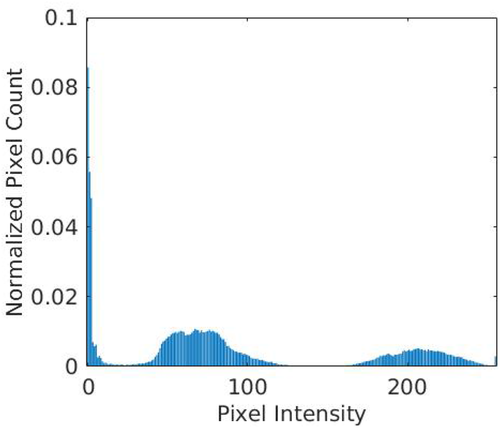
\includegraphics[scale=0.80]{doc_images/histograma_intensidad.png}
		\caption{Histograma normalizado de ambas imágenes de fondo de ojo. Fuente: \parencite{piyasena2018}.} 
		\label{fig:Histograma_Intensidades}
	\end{figure}
\end{center}

\begin{center}
	\begin{figure}[H]
		\centering
		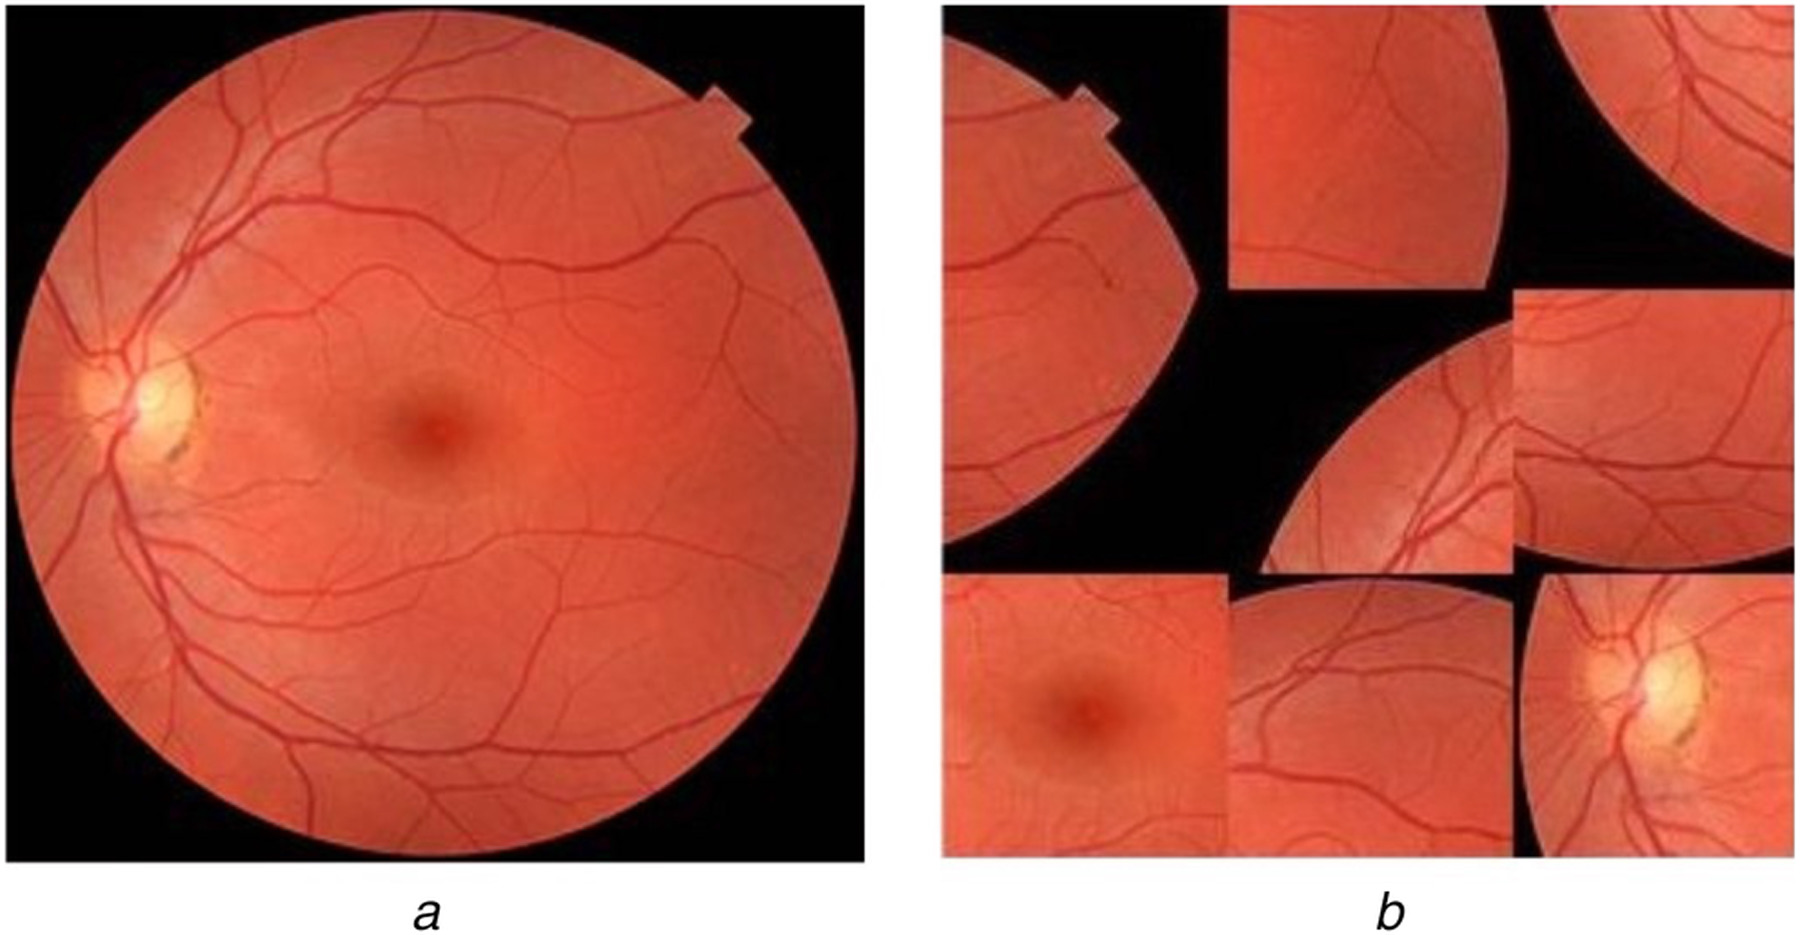
\includegraphics[scale=0.30]{doc_images/retina_del_histograma.jpg}
		\caption{Imágenes de fondo de ojo. (a) Buena calidad, (b) Mala calidad. Fuente: \parencite{piyasena2018}.} 
		\label{fig:retina_del_histograma}
	\end{figure}
\end{center}

Otros modelos se basaron en métodos de segmentación para detectar las diferentes estructuras del ojo (Figura \ref{fig:macula_do_vasos}). Inicialmente, la cantidad de píxeles asociados a los vasos sanguíneos se utilizaba como indicador de calidad, asumiendo que una mayor cantidad indicaba una mejor calidad. Posteriormente, se introdujeron mejoras, como el análisis de los vasos sanguíneos alrededor de la mácula, estructuras pequeñas y estrechas que son especialmente susceptibles a distorsiones y, por tanto, útiles como medida de calidad. También se incorporó la evaluación de la posición absoluta de la fóvea\footnote{Fóvea: Pequeña depresión en el centro de la mácula responsable de la visión aguda y detallada.} y la distancia promedio de los vasos respecto a esta. Finalmente, para abordar el problema del desenfoque, se utilizó el contraste entre los vasos sanguíneos y el fondo como indicador principal de nitidez. Aunque estos algoritmos reflejan con mayor precisión el enfoque utilizado por los oftalmólogos para evaluar la calidad de las imágenes, también presentan ciertos inconvenientes al intentar generalizarlos. Por un lado, operan bajo supuestos fijos sobre la forma, tamaño y posición de las estructuras del ojo, lo que puede limitar su desempeño al analizar imágenes que no se ajusten a esas características. Por otro lado, aunque incluyen el manejo de ruido, como el desenfoque, suelen estar diseñados para tratar tipos específicos de ruido, lo que significa que podrían fallar al enfrentarse a ruidos distintos de los previstos durante su desarrollo.

\begin{center}
	\begin{figure}[ht]
		\centering
		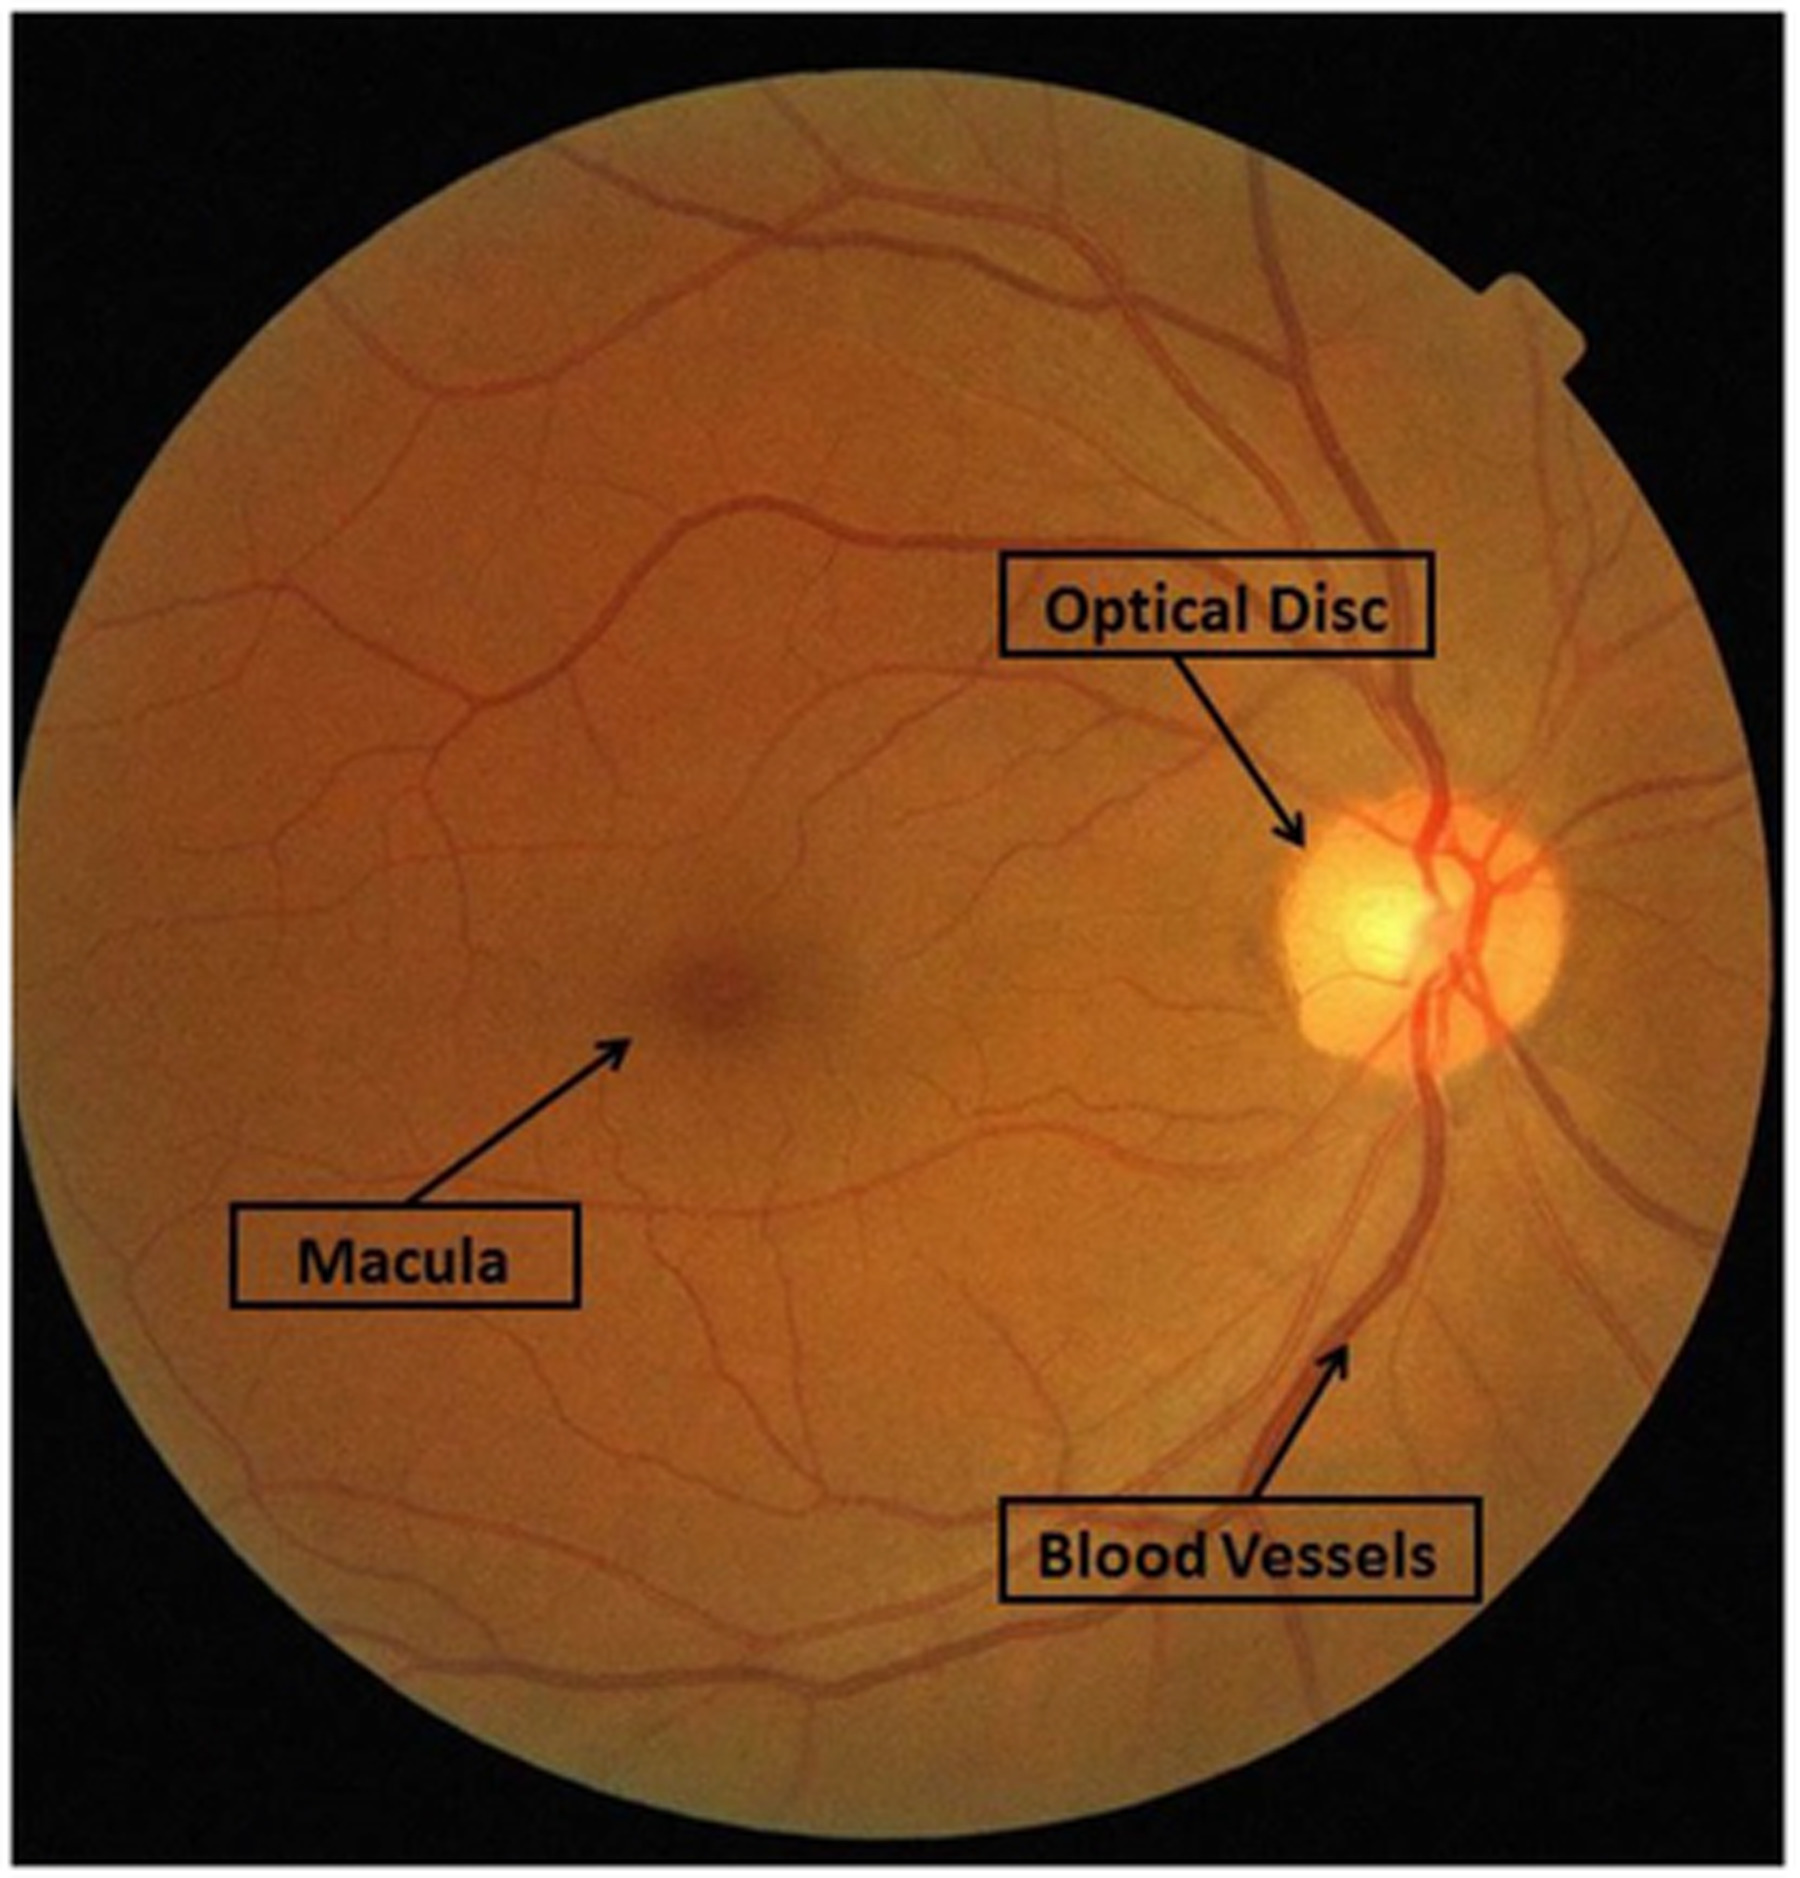
\includegraphics[scale=0.15]{doc_images/macula_do_vasos.jpg}
		\caption{Imagen de fondo de ojo donde se pueden observar las estructuras principales: mácula, disco óptico y vasos sanguíneos. Fuente: \parencite{piyasena2018}.} 
		\label{fig:macula_do_vasos}
	\end{figure}
\end{center}

Tanto las medidas de similitud como los métodos de segmentación fueron luego combinados y refinados para ser utilizados como predictores para entrenar diferentes algoritmos de machine learning, como SVM, regresión o k-NN, con el fin de realizar una clasificación binaria, multiclase o asignar un puntaje de calidad \parencite{piyasena2018}.
Los métodos basados en atributos hechos a mano dependen en gran medida del diseño de características, siendo demasiado complejo lograr características eficientes y apropiadas que se adapten a las variaciones y complejidades inherentes a las imágenes oftalmológicas \parencite{xu2020}. Esto genera limitaciones en el rendimiento, especialmente en condiciones no previstas o en imágenes con artefactos y ruidos inesperados.

\section{Métodos basados en la extracción automática de características}
Los métodos basados en redes neuronales han emergido como una solución innovadora para superar las limitaciones inherentes a los enfoques tradicionales en la evaluación de la calidad de imágenes de fondo de ojo. A diferencia de los métodos que dependen del diseño manual de características, las redes neuronales tienen la capacidad de aprender representaciones directamente a partir de los datos, eliminando la necesidad de intervención manual en la extracción de atributos. Esto es particularmente relevante, dado que la selección de características en los enfoques tradicionales es un proceso complejo, sujeto a sesgos y, a menudo, incapaz de capturar la diversidad de variaciones presentes en las imágenes clínicas. Las redes neuronales no solo automatizan este proceso, sino que también permiten identificar patrones complejos que los métodos tradicionales no pueden capturar. Además, logran distinguir entre características relevantes y artefactos irrelevantes, mejorando tanto la precisión como la robustez frente a variaciones en las condiciones de captura, como el desenfoque o los niveles de iluminación.

En 2016, \cite{mahapatra2016} propusieron el primer algoritmo basado en CNN para evaluar la calidad de imágenes de fondo de ojo. Sin embargo, se enfrentaron a dos desafíos: la escasa cantidad de imágenes para el entrenamiento (solo 101) y la falta de imágenes de mala calidad. Para superar estos problemas, extrajeron parches de 150×150 píxeles de las imágenes, etiquetándolos igual que las imágenes originales. Además, simularon distorsiones, como el ruido gaussiano, para generar imágenes de baja calidad que complementaran su conjunto de datos. De manera similar, \cite{costa2017eyequal} emplearon la técnica de dividir las imágenes en subregiones para clasificar cada una por separado y luego ponderar los resultados, obteniendo una clasificación final para la imagen completa.

El principal inconveniente de ambos enfoques es el tamaño reducido de la muestra, lo que dificulta el entrenamiento efectivo de una red neuronal. Para abordar este problema, \cite{yu2017image} utilizaron una CNN para extraer características, pero no para realizar la clasificación directamente. En su lugar, combinaron las salidas de la CNN con características manualmente construidas y utilizaron un SVM para clasificar las imágenes como de buena o mala calidad.

Uno de los principales desafíos al utilizar redes neuronales es la necesidad de grandes cantidades de datos etiquetados, lo cual es costoso y laborioso de obtener. Por esta razón, en los últimos años se ha explorado el uso de redes preentrenadas como una posible solución. Al aprovechar modelos previamente entrenados en grandes bases de datos, incluso si son imágenes naturales, los investigadores pueden realizar un fine-tuning para adaptarlos a tareas específicas, como la clasificación de calidad de imágenes retinianas. En este sentido, \cite{saha2018automated} utilizan la arquitectura AlexNet, inicializada con pesos preentrenados del modelo de referencia de Caffe\footnote{Caffe: Convolutional Architecture for Fast Feature Embedding, es un marco de aprendizaje profundo que admite una variedad de arquitecturas de aprendizaje profundo e incluye modelos preentrenados.} (entrenado en ImageNet\footnote{ImageNet:  Base de datos extensa con más de 14 millones de imágenes etiquetadas, utilizada ampliamente en la investigación de modelos de reconocimiento de objetos y entrenamiento de redes neuronales.}) y después realizan un fine-tuning para la evaluación de calidad de las retinografías. La arquitectura AlexNet consta de cinco capas convolucionales: la primera tiene 96 filtros de 11x11, la segunda 256 filtros de 5x5, la tercera y cuarta 384 filtros de 3x3, y la última 256 filtros de 3x3. Posteriormente, la red incluye dos capas completamente conectadas de 4096 neuronas cada una, seguidas de una capa completamente conectada de 1000 neuronas.  \cite{saha2018automated} reemplazan esta última capa por un clasificador binario para adaptar la red a su problema específico.

\begin{center}
	\begin{figure}[h]
		\centering
		
\includegraphics[scale=0.15]{doc_images/AlexNet_Original_block_diagram.svg.png}
		\caption{Arquitectura de la red neural convolucional AlexNet. Fuente: \parencites{krizhevsky2012imagenet}.} 
		\label{fig:AlexNet_Original_block_diagram}
	\end{figure}
\end{center}

En una línea similar, \cite{zago2018retinal} aplican la técnica de fine-tuning en una CNN VGG-16, una red más profunda con 16 capas en lugar de 8, que utiliza filtros más pequeños. Además, emplean distintos conjuntos de datos para el entrenamiento y la validación. De esta forma, haciendo validación cruzada dentro de cada conjunto y entre diferentes datasets, permite evaluar la capacidad del modelo para generalizar a datos provenientes de diversas fuentes.

\begin{center}
	\begin{figure}[H]
		\centering
		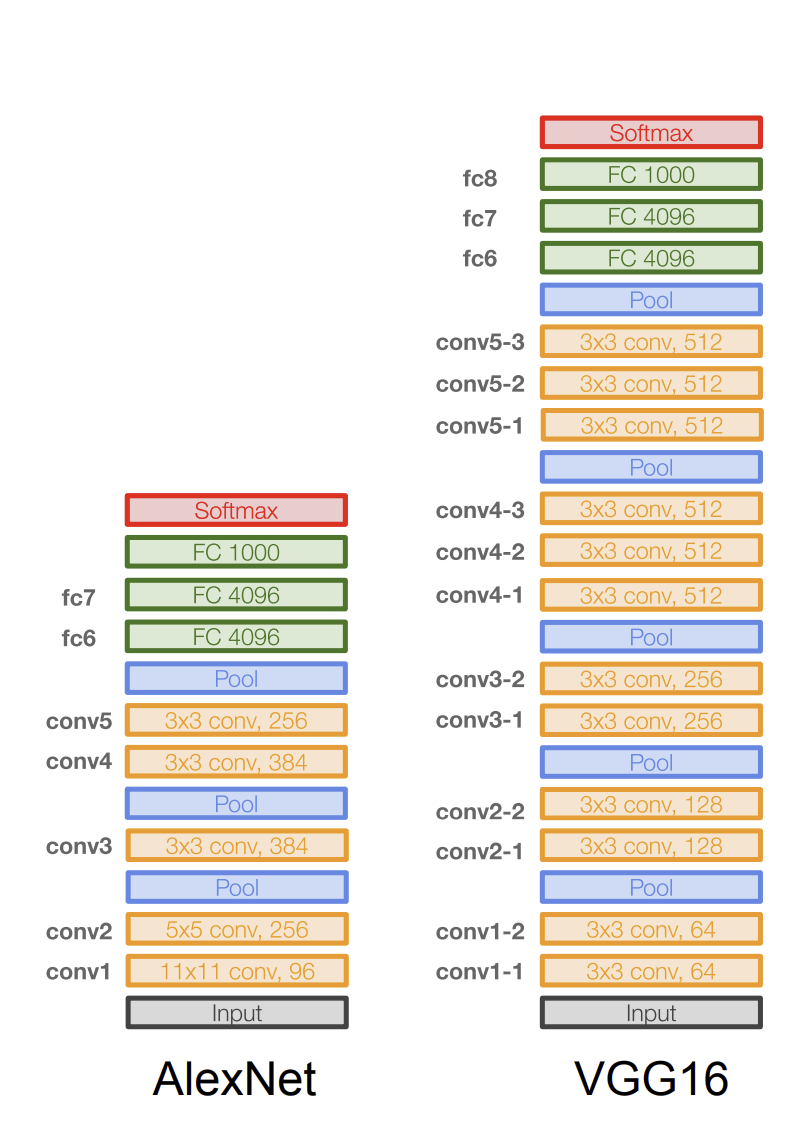
\includegraphics[scale=0.80]{doc_images/AlexNet_VGG16.png}
		\caption{Comparación entre arquitecturas de redes AlexNet y VGG16. Extraído de Convolutional Neural Networks for Visual Recognition [Diapositivas del curso], por K. Li, A. Karpathy, y J. Johnson, 2020, Universidad de Stanford, \url{https://cs231n.stanford.edu/slides/2020/lecture_9.pdf}.} 
		\label{fig:AlexNet_VGG16}
	\end{figure}
\end{center}

\cite{fu2019evaluation} analizan la influencia de los distintos espacios de color en la evaluación de calidad de imágenes retinianas, proponiendo una arquitectura llamada Multiple Color-space Fusion Network (MCF-Net). Esta red consta de dos bloques: un bloque base donde entrenan tres CNN en paralelo para cada uno de los espacios de color (RGB, HVS, LAB), generando un mapa de características para cada uno, y un segundo bloque donde fusionan la salida de las tres redes en una sola representación. Esta fusión de los tres canales junto con cada una de las representaciones individuales se utilizan como entrada para realizar la clasificación final. \cite{fu2019evaluation} demuestran que el rendimiento es superior cuando se consideran múltiples canales de color en comparación con el rendimiento de cada canal individualmente.

\begin{center}
	\begin{figure}[H]
		\centering
		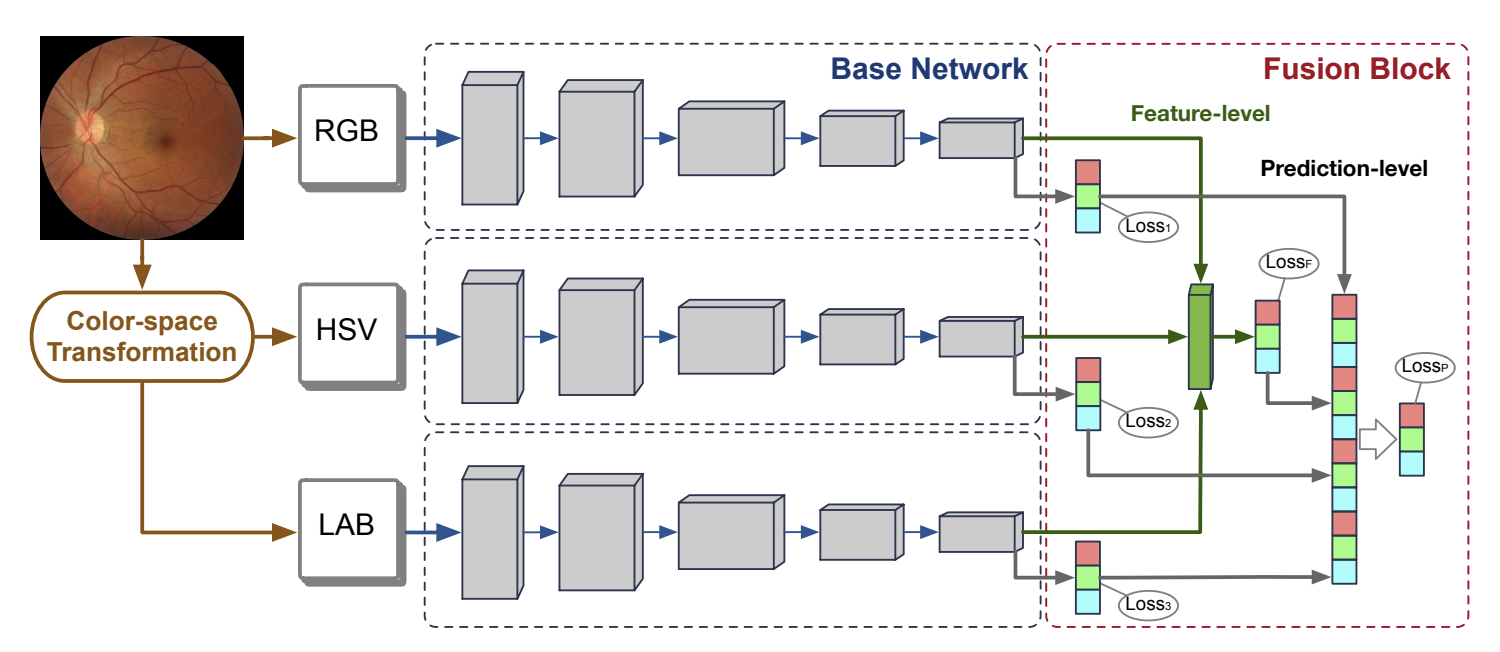
\includegraphics[scale=0.80]{doc_images/FU.png}
		\caption{Arquitectura MCF-Net \parencites{fu2019evaluation}.} 
		\label{fig:FU}
	\end{figure}
\end{center}

En este contexto, \cite{shen2018multi} afirman que las tareas auxiliares contribuyen a la evaluación de la calidad de las imágenes retinianas y proponen un marco de trabajo multi-tarea denominado Multi-task Fundus Image Quality Assessment (MFIQA).En este marco, una ResNet50, una red neuronal profunda que utiliza conexiones residuales para facilitar el entrenamiento de redes con muchas capas, se entrena para la detección del disco óptico y la mácula, mientras que una VGG16 se emplea para refinar la localización de estas estructuras. Además, se utilizan dos codificadores: uno para codificar imágenes retinianas completas en un sistema de coordenadas cartesianas, y otro para codificar ventanas locales del disco óptico en un sistema de coordenadas polares para la clasificación de la calidad de las imágenes. El modelo es entrenado para tres tareas auxiliares de clasificación de artefactos, claridad y definición de campo, que ayudan en el aprendizaje de la evaluación de calidad.

\begin{center}
	\begin{figure}[H]
		\centering
		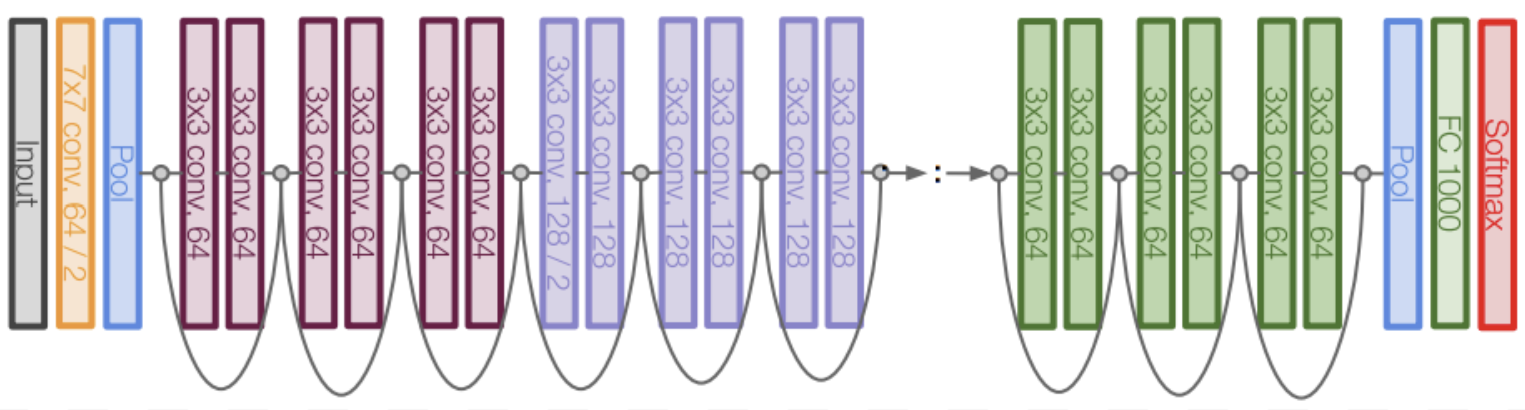
\includegraphics[scale=0.80]{doc_images/resnet.png}
		\caption{Arquitectura de redes residuales (ResNet) que puede tener 18, 34, 50, 101 o 152 capas. Extraído de Convolutional Neural Networks for Visual Recognition [Diapositivas del curso], por K. Li, A. Karpathy, y J. Johnson, 2020, Universidad de Stanford, \url{https://cs231n.stanford.edu/slides/2020/lecture_9.pdf}.} 
		\label{fig:resnet}
	\end{figure}
\end{center}

Tanto MCF-Net como MFIQA agregan características ricas que mejoran la clasificación, aunque en ambas arquitecturas, los parámetros a optimizar aumentan considerablemente. Además, el aprendizaje de tareas auxiliares requiere más anotaciones sobre las imágenes, lo cual resulta costoso \parencites{xu2020deep}. En este contexto, \cite{xu2020deep} retoman los fundamentos al destacar los elementos que los oftalmólogos consideran esenciales en una retinografía para evaluar su calidad. Su enfoque se centra en la detección de estructuras relevantes, diferenciando entre aquellas de pequeño tamaño, como los vasos sanguíneos, y las de mayor tamaño, como la mácula o el disco óptico. Estas estructuras se combinan con la imagen original para servir como entrada en el aprendizaje profundo de características y la posterior clasificación de calidad. Para incorporar estos priors\footnote{Priors: Información previa que se incorpora al modelo para guiar el proceso de aprendizaje.} de estructuras relevantes, proponen el modelo SalStructIQA (Salient Structure Image Quality Assessment), que tiene dos variantes: una de rama única y otra de dos ramas. En la primera, se concatenan la imagen original y los mapas de características de las estructuras pequeñas y grandes antes de proceder al aprendizaje profundo para la clasificación de calidad. En la variante de dos ramas, se utilizan dos CNN paralelas que aprenden separadamente las características de la imagen retiniana con estructuras grandes y pequeñas, fusionando posteriormente estas características para la evaluación de calidad.

\begin{center}
	\begin{figure}[H]
		\centering
		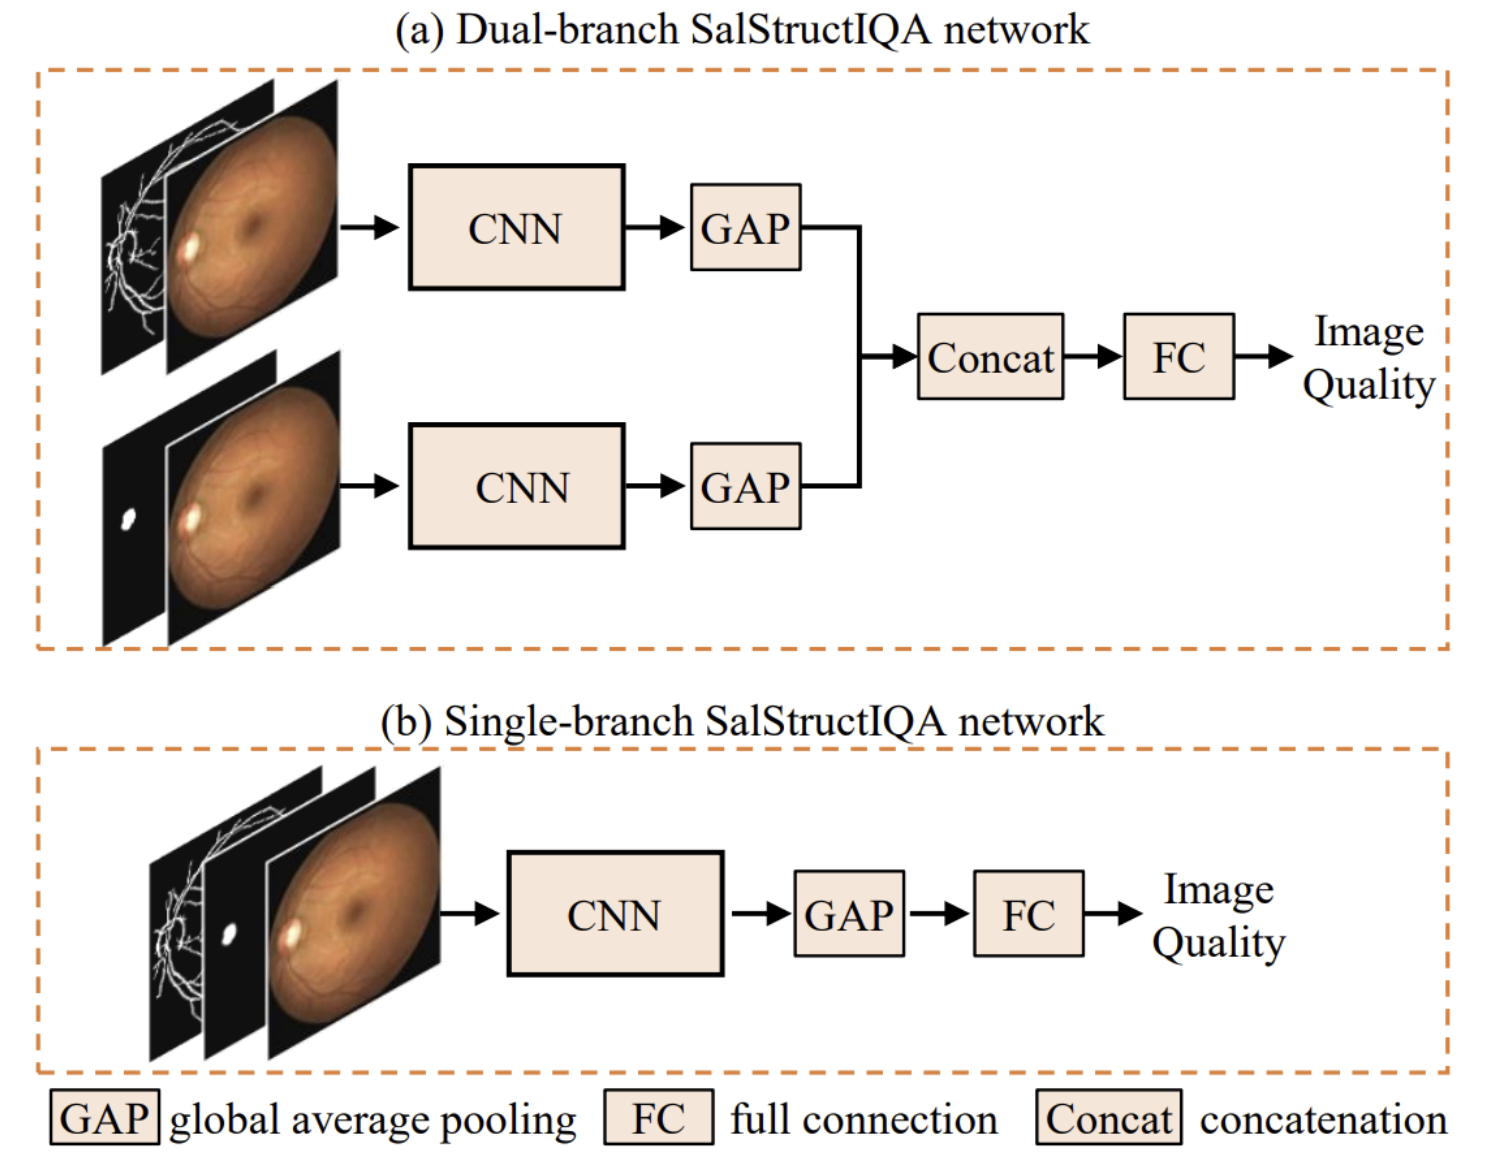
\includegraphics[scale=0.80]{doc_images/SalStructl.png}
		\caption{Dos implementaciones de la arquitectura SalStructlQA, \parencites{xu2020deep}.} 
		\label{fig:SalStructl}
	\end{figure}
\end{center}

En el cuadro \ref{tab:metodosQA}, que se encuentra en el anexo, se detallan los métodos de evaluación de calidad de imágenes de fondo de ojo.


	\chapter{Datasets utilizados}

\section{High-Resolution Fundus (HRF)}
Consiste en 18 pares de imágenes de la misma retina, capturadas con una cámara Canon CR-1 con un campo de visión de 45°. Cada par contiene una imagen de mala calidad y una imagen de mejor calidad, representando situaciones en las que la exploración tuvo que repetirse debido a deficiencias en la adquisición.

Las imágenes de baja calidad presentan problemas como desenfoque global o localizado, generalmente causado por un enfoque incorrecto de la cámara. Ambas imágenes de cada par comparten aproximadamente el mismo campo visual, aunque pueden presentar pequeños desplazamientos debido a movimientos involuntarios del ojo durante la captura. El nombre de cada archivo corresponde con el número identificador de la retina y la etiqueta de calidad \parencites{koehler2013automatic}.

\begin{center}
	\begin{figure}[H]
		\centering
		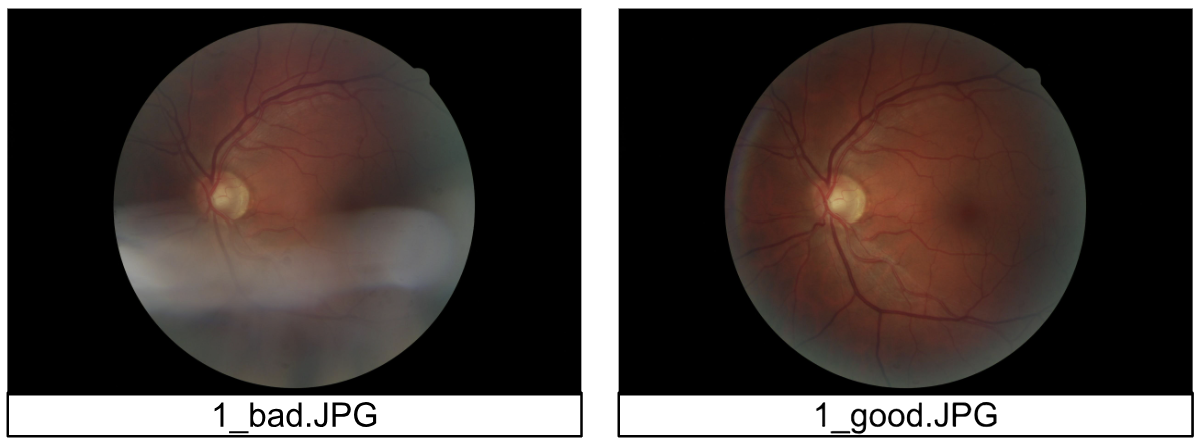
\includegraphics[scale=0.80]{doc_images/HRF.png}
		\caption{Ejemplo de imágenes de fondo de ojo del dataset HRF.} 
		\label{fig:HRF}
	\end{figure}
\end{center}

\section{DDR}
Contiene 13,673 imágenes en color de fondo de ojo obtenidas entre 2016 y 2018 de 9,598 pacientes en 147 hospitales de 23 provincias de China. La recopilación siguió criterios de distribución uniforme en cuanto a edad, género y procedencia geográfica de los pacientes, asegurando la diversidad en el conjunto de datos.

Las imágenes fueron capturadas con 42 tipos de cámaras de fondo de ojo con un campo de visión de 45°, incluyendo modelos como Topcon D7000, Topcon TRC NW48, Nikon D5200 y Canon CR-2.

Cada imagen fue etiquetada por siete especialistas según la Clasificación Internacional de Retinopatía Diabética, asignándolas a una de seis categorías: No DR, DR no proliferativa leve, DR no proliferativa moderada, DR no proliferativa severa, DR proliferativa, No calificable (imágenes con más del 70\% de desenfoque y sin lesiones claramente visibles).

La categorización de las imágenes siguió un proceso de votación entre los especialistas. En caso de desacuerdo, se consultaron oftalmólogos con más de 30 años de experiencia para la decisión final.

\begin{center}
	\begin{figure}[H]
		\centering
		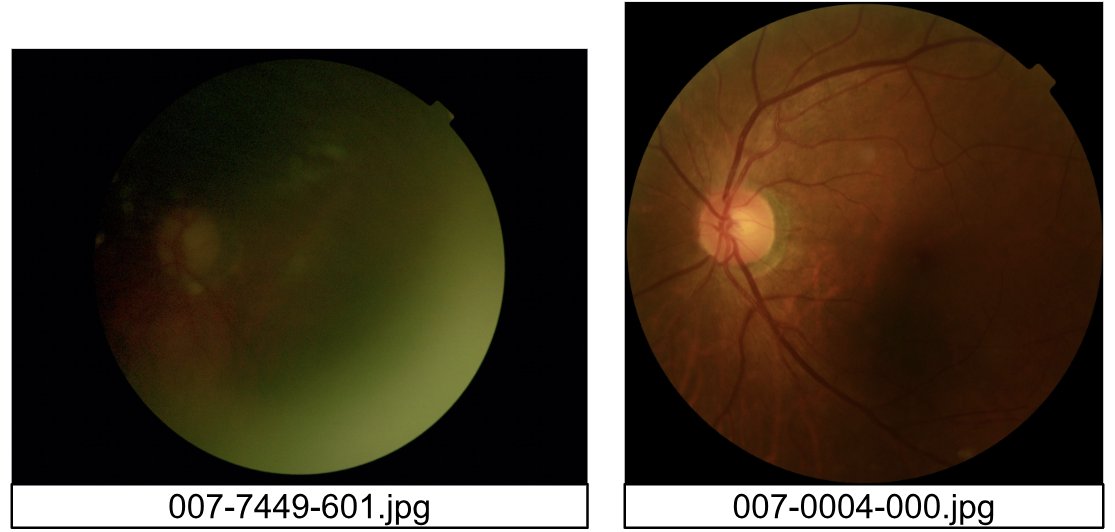
\includegraphics[scale=0.80]{doc_images/DDR.png}
		\caption{Ejemplo de imágenes de fondo de ojo del dataset DDR, (izquierda: No clasificable, derecha: No DR).} 
		\label{fig:DDR}
	\end{figure}
\end{center}

\section{Deep Diabetic Retinopathy Image Dataset (DeepDRiD)}
El DeepDRiD es un conjunto de datos desarrollado para la competencia Diabetic Retinopathy: Segmentation and Grading Challenge, organizada en conjunto con el Simposio Internacional de IEEE sobre Imágenes Biomédicas (ISBI 2020). Su propósito es evaluar métodos de clasificación automática de la retinopatía diabética (DR) y la calidad de imágenes de fondo de ojo.

El dataset está compuesto por imágenes obtenidas de pacientes incluidos en diferentes estudios en Shanghai, como el Shanghai Diabetic Complication Screening Project, el Nicheng Diabetes Screening Project y el Nation-wide Screening for Complications of Diabetes. Además, se incorporaron imágenes adquiridas en la clínica de oftalmología del Sixth People’s Hospital of Shanghai Jiao Tong University. De los miles de exámenes disponibles, se seleccionaron aleatoriamente 2.000 imágenes de fondo de ojo regulares correspondientes a 500 pacientes. Cada paciente tiene cuatro imágenes de fondo de ojo, con dos imágenes por ojo: una centrada en la mácula y otra en el disco óptico.

Las imágenes se separaron 60\% (1.200 imágenes) para entrenamiento, 20\% (400 imágenes) para validación y 20\% (400 imágenes) para evaluación. Las imágenes de este dataset están etiquetadas en un archivo CSV, donde la variable Overall quality indica la calidad de la imagen: 0 para imágenes de mala calidad y 1 para imágenes de buena calidad (Liu et al., 2022). En este trabajo, solo se utilizan los conjuntos de entrenamiento y validación, ya que para el conjunto de evaluación no están disponibles las etiquetas. Las 1.600 imágenes se utilizarán exclusivamente para la fase de prueba, sin formar parte del entrenamiento del modelo.

\begin{center}
	\begin{figure}[H]
		\centering
		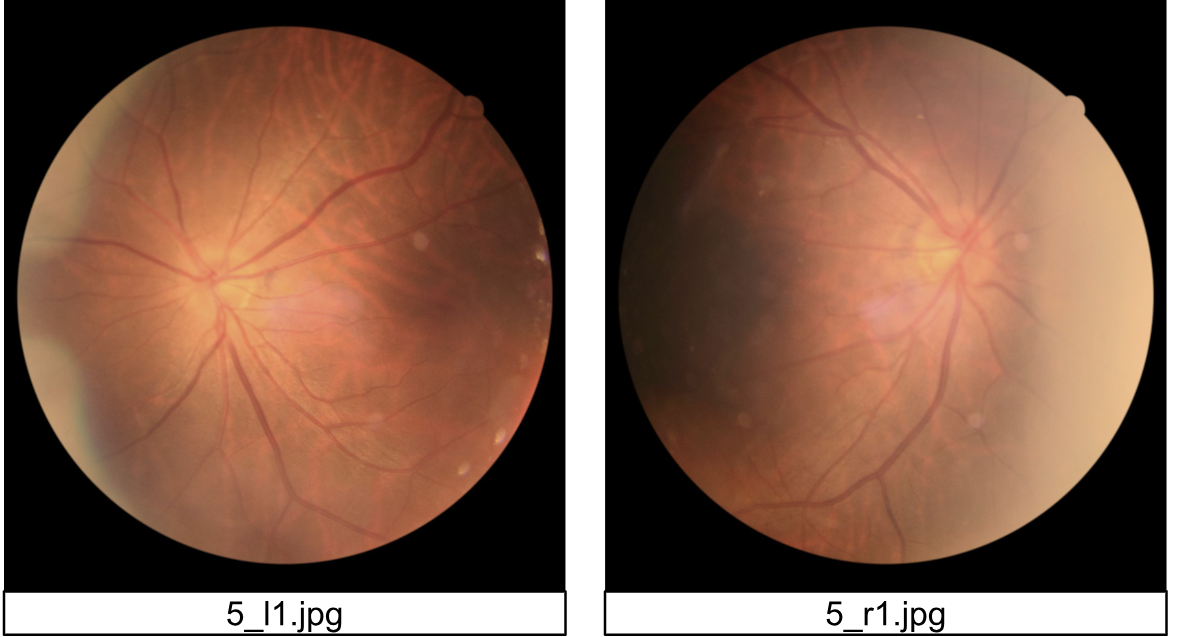
\includegraphics[scale=0.80]{doc_images/DeepDRiD.png}
		\caption{Ejemplo de imágenes de fondo de ojo del dataset DeepDRiD, (izquierda: buena calidad, derecha: mala calidad).} 
		\label{fig:DeepDRiD}
	\end{figure}
\end{center}

\section{Kaggle DR Dataset}
Este conjunto de datos contiene imágenes de retina proporcionadas por EyePACS\footnote{EyePACS: es una red de telemedicina que proporciona acceso a exámenes de retina para la detección de retinopatía diabética y otras enfermedades oculares. \url{https://eyepacs.com/}} para la competencia organizada por Kaggle\footnote{\url{https://www.kaggle.com/c/diabetic-retinopathy-detection/overview}} y la California Healthcare Foundation, con el objetivo de desarrollar modelos de detección de retinopatía diabética. Contiene miles de imágenes capturadas con diferentes modelos y tipos de cámaras, con variaciones en términos de iluminación, enfoque y calidad en general. Sin embargo, este conjunto de datos no incluye etiquetas explícitas de calidad de imagen.

Para obtener etiquetas de calidad, se utilizó la versión etiquetada por profesionales propuesta por \parencites{zhou2018deep}, denominada Kaggle DR Image Quality Dataset, en la que las imágenes fueron clasificadas en dos categorías: 0 para imágenes de mala calidad y 1 para imágenes de buena calidad. Este conjunto de datos está dividido en 35,126 imágenes para entrenamiento, 10,906 para validación y 42,670 para evaluación. Las etiquetas de calidad están almacenadas en archivos CSV, con un archivo separado para cada partición (entrenamiento, validación y evaluación). Cada CSV contiene el nombre de la imagen y su respectiva etiqueta en el campo quality.


\begin{center}
	\begin{figure}[H]
		\centering
		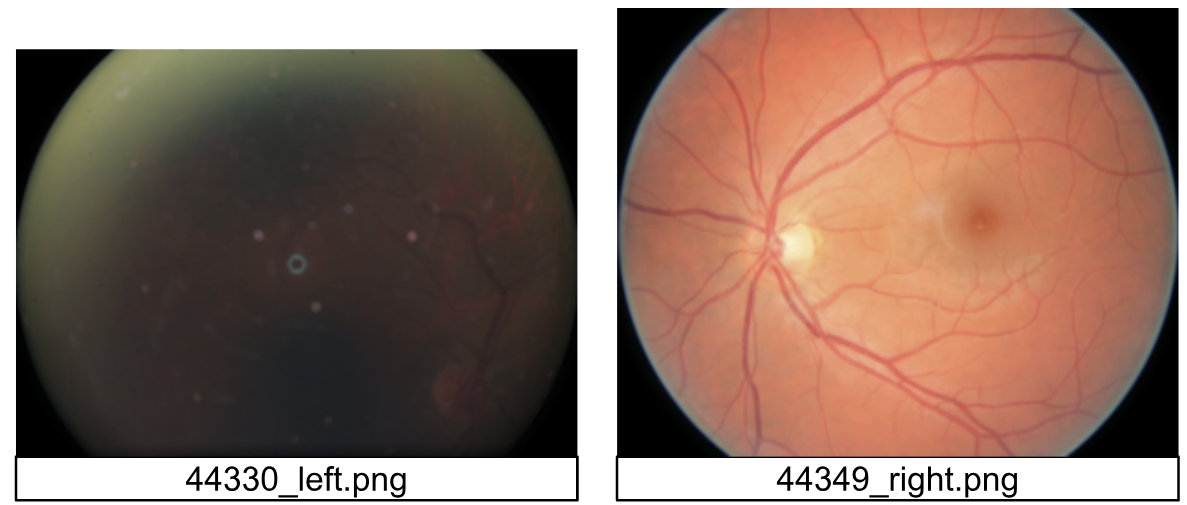
\includegraphics[scale=0.80]{doc_images/Kaggle.png}
		\caption{Ejemplo de imágenes de fondo de ojo del dataset Kaggel, (izquierda: mala calidad, derecha: buena calidad).} 
		\label{fig:Kaggle}
	\end{figure}
\end{center}

El cuadro \ref{tab:dataset_count} presenta un resumen con la cantidad de imágenes utilizadas en los subconjuntos de entrenamiento, validación y test.

\begin{table*}[h]
	\centering
	\renewcommand{\arraystretch}{1.5}
	\resizebox{\textwidth}{!}{
	\begin{tabular}{ |c|c|c|c|c|c|c|c|c|c|  }
		\hline
		\multirow{2}{*}{\textbf{Dataset}}&\multicolumn{3}{|c|}{\textbf{Train}} &\multicolumn{3}{|c|}{\textbf{Validation}} &\multicolumn{3}{|c|}{\textbf{Test}} \\
		\cline{2-10}
		 & \textbf{Buena} & \textbf{Mala} & \textbf{Total} & \textbf{Buena} & \textbf{Mala} & \textbf{Total} & \textbf{Buena} & \textbf{Mala} & \textbf{Total} \\
		\hline
		HRF & 9 & 9 & 18 & 6 & 6 & 12 & 3 & 3 & 6 \\
		\hline
		DDR & 6,260 & 575 & 6,835 & 2,503 & 230 & 2,733 & 3,759 & 346 & 4,105 \\
		\hline
		DeepDRiD & - & - & - & - & - & - & 758 & 842 & 1,600 \\
		\hline
		Kaggle & 33,840 & 1,285 & 35,125 & 10,680 & 226 & 10,906 & 41,797 & 873 & 42,670 \\
		\hline
		\hline
		Total & 40,109 & 1,869 & 41,978 & 13,189 & 462 & 13,651 & 46,317 & 2,064 & 48,381 \\
		\hline
	\end{tabular}
	}
	\caption{Distribución de imágenes por dataset, clase y partición.}
	\label{tab:dataset_count}
\end{table*}
	\chapter{Metodología}

\section{Preprocesamiento de imágenes}
\subsection{Normalización del fondo}
Variaciones en el color del fondo pueden afectar la capacidad del modelo para aprender características relevantes, desviando su atención hacia patrones irrelevantes. Por ello, se aplica un proceso de normalización del fondo, asegurando que la información procesada esté centrada en la región de interés y no en elementos circunstanciales de la adquisición de la imagen.
En primer lugar, la imagen original se convierte a escala de grises utilizando la transformación de OpenCV\footnote{OpenCV. (s.f.). Open Source Computer Vision Library. OpenCV Documentation. \url{https://docs.opencv.org/}}:

\[
RGB[A] \;to \;Gray: Y \leftarrow 0.299 \cdot R \;+\; 0.587 \cdot G \;+\; 0.114 \cdot B
\]

donde R,G,B son los valores de los canales rojo, verde y azul respectivamente.
Luego, se calcula la distribución de intensidades mediante un conteo de frecuencias de los valores de píxeles. Si la intensidad con mayor frecuencia corresponde a 255, se infiere que el fondo de la imagen es blanco. En este caso, todos los píxeles con valor 255 en la imagen original son reemplazados por 0 (negro). En caso contrario, la imagen se mantiene sin modificaciones.

\begin{center}
	\begin{figure}[H]
		\centering
		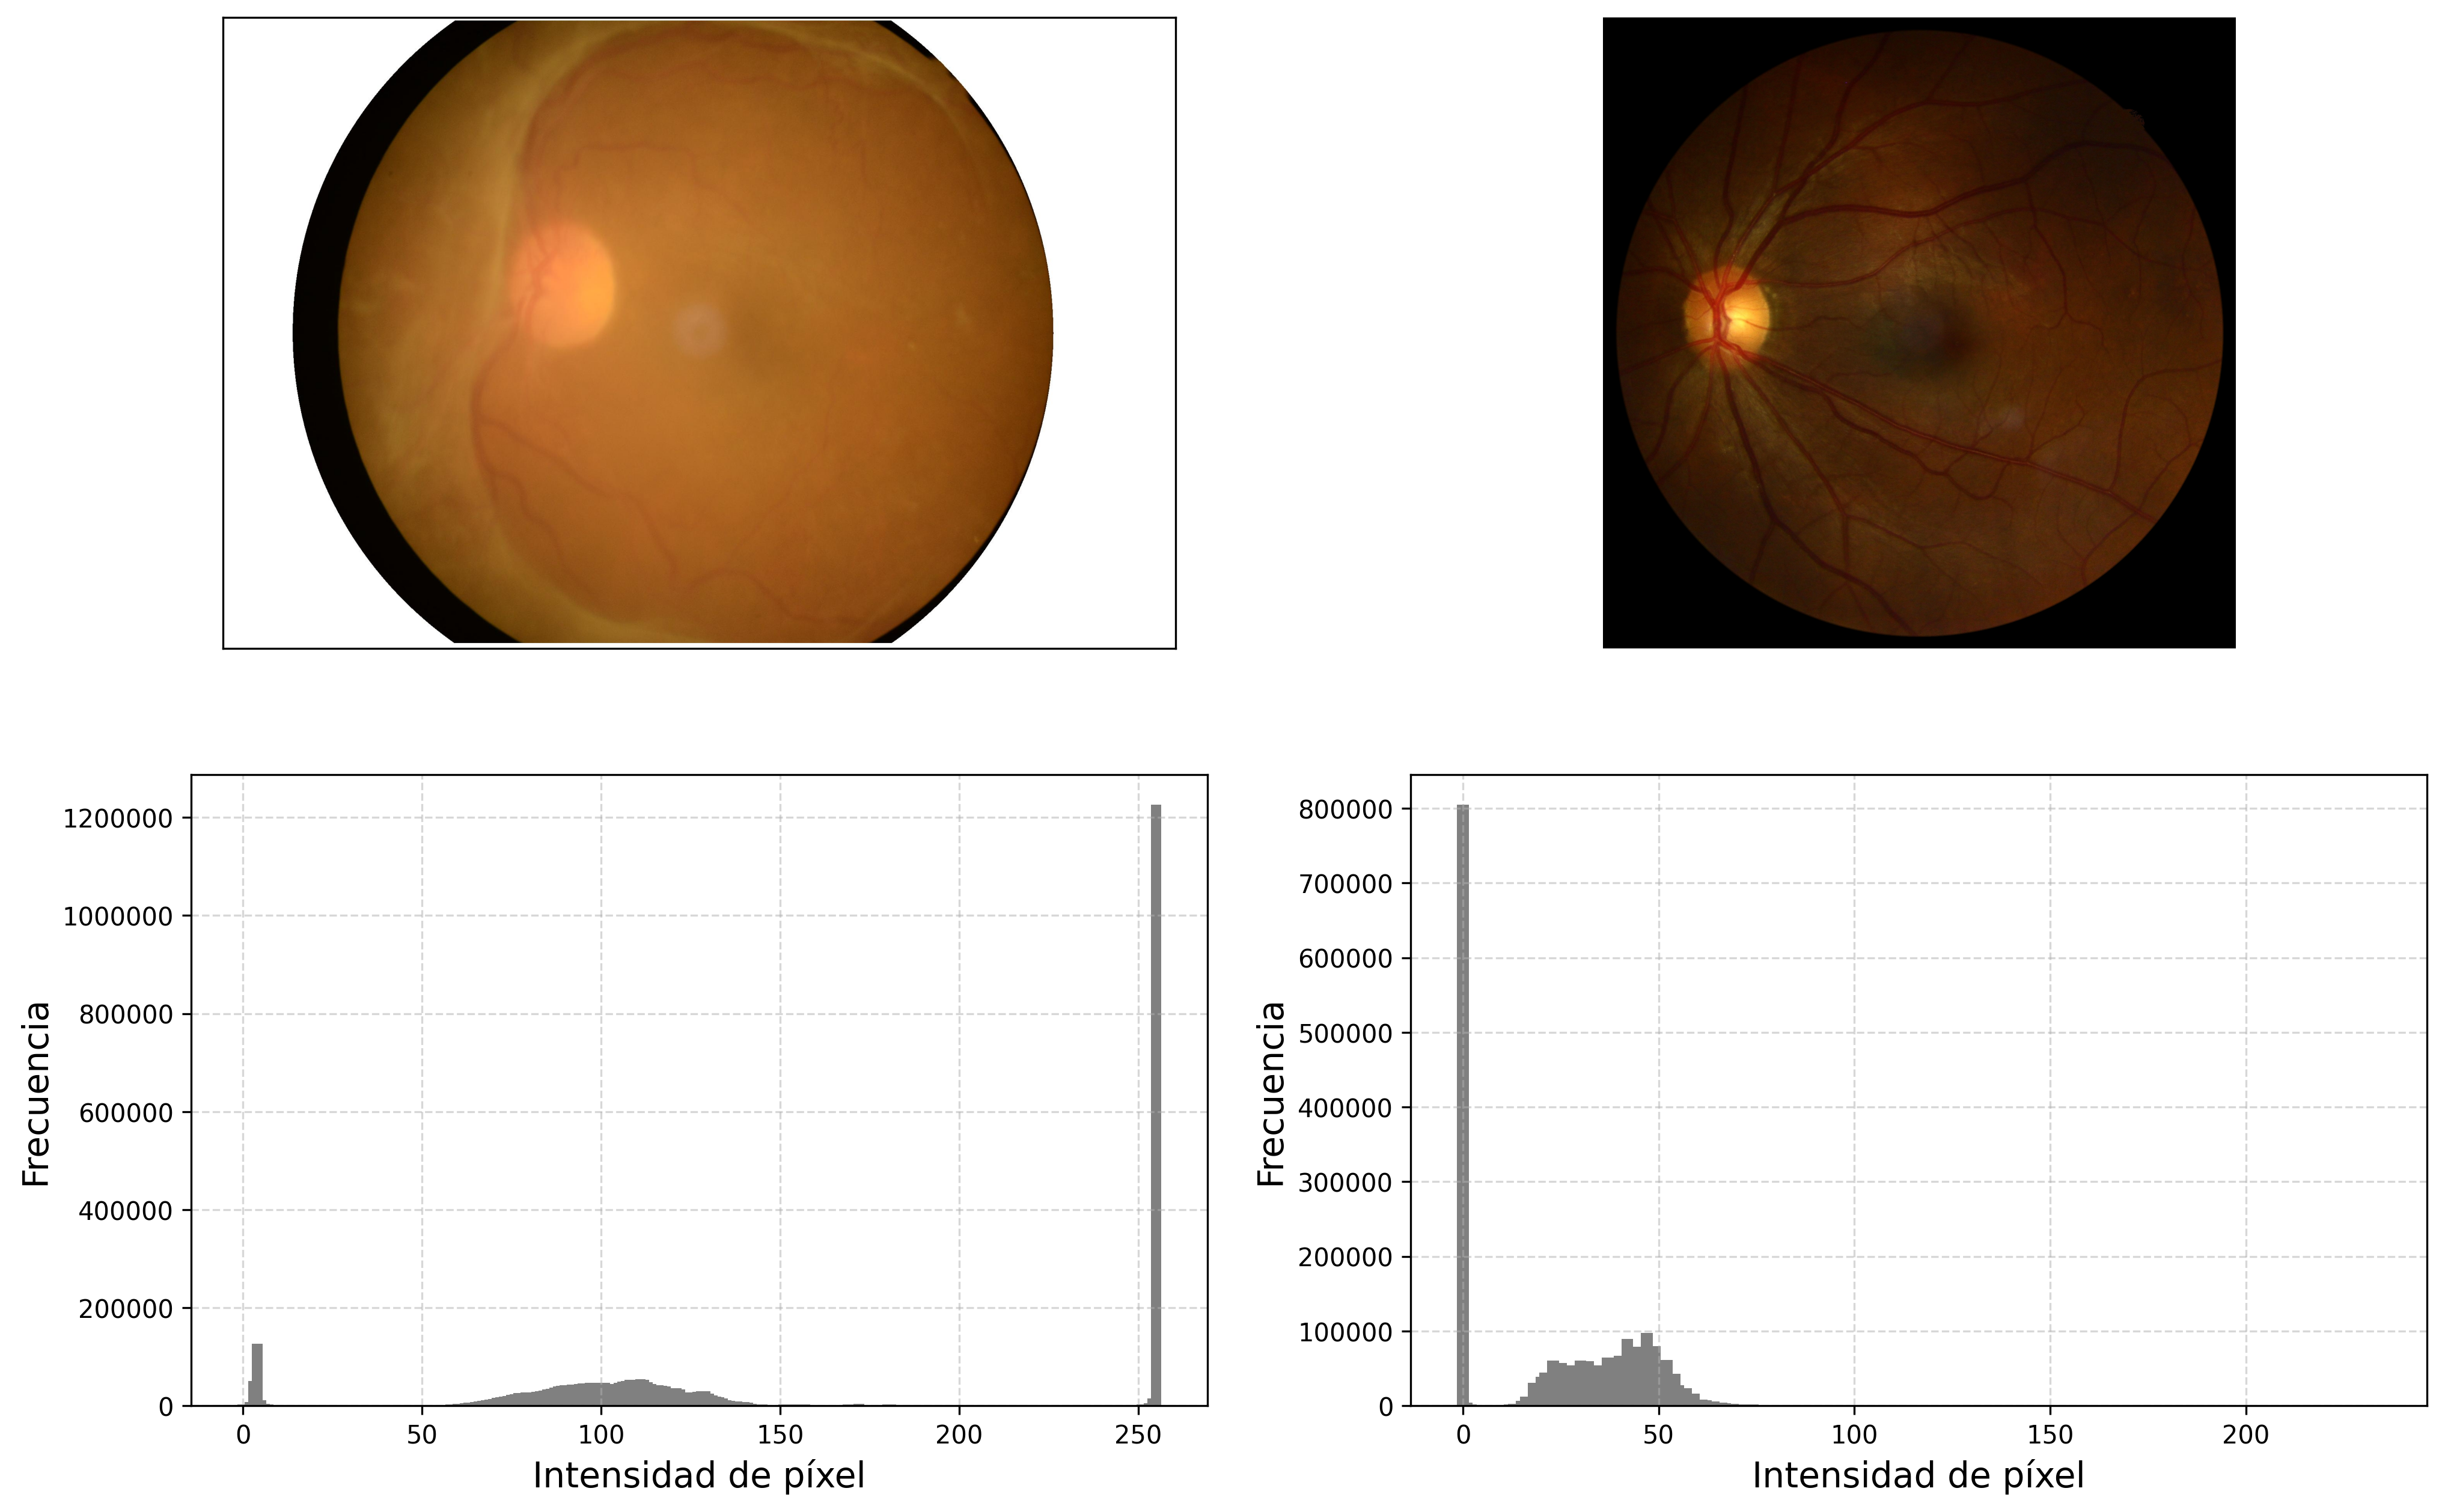
\includegraphics[scale=0.40]{doc_images/histograma_con_imagenes.png}
		\caption{Comparación de dos imágenes de fondo de ojo (izquierda: fondo blanco, derecha: fondo negro) y sus respectivos histogramas de intensidad en escala de grises.} 
		\label{fig:histograma_con_imagenes}
	\end{figure}
\end{center}

\begin{center}
	\begin{figure}[H]
		\centering
		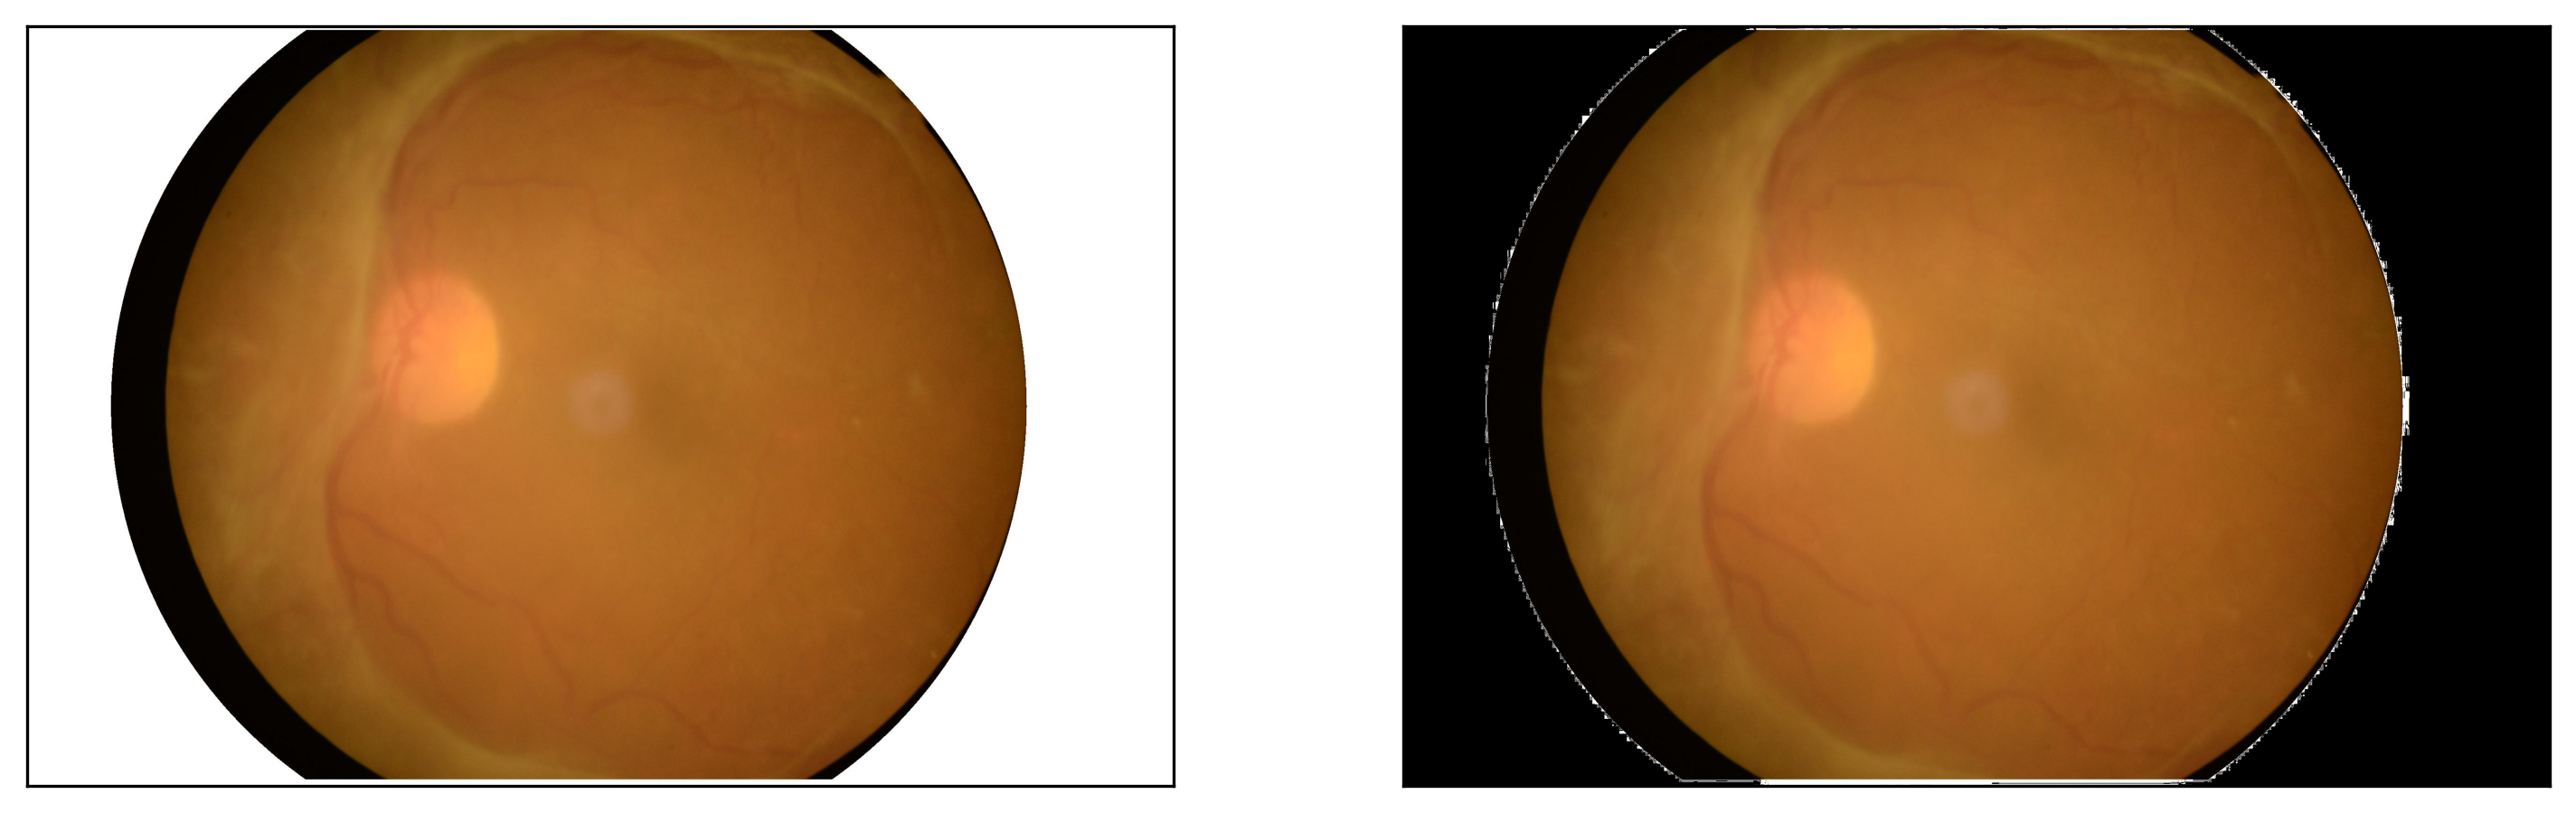
\includegraphics[scale=0.60]{doc_images/fondo_blanco_a_negro.png}
		\caption{Imagen original (izquierda) y versión modificada (derecha), donde los píxeles de fondo blanco (valor 255) fueron reemplazados por negro (valor 0).} 
		\label{fig:fondo_blanco_a_negro}
	\end{figure}
\end{center}

\subsection{FOV (Field of View)}
Dado que la región de interés en estas imágenes presenta una forma circular bien definida, se emplea un método basado en la detección de círculos para segmentar el campo de visión (FOV) en la imagen de fondo de ojo.

Inicialmente, la imagen se convierte a escala de grises y se aplica un filtro de desenfoque de mediana\footnote{Filtro de desenfoque de mediana: técnica digital que se usa para reducir el ruido en imágenes, videos y señales, preservando bordes y esquinas redondeadas.} para reducir el ruido sin perder bordes significativos. Luego, se intenta detectar un círculo en la imagen mediante la transformada de Hough\footnote{La transformada de Hough busca estructuras circulares en imágenes en escala de grises al analizar bordes y acumular votos en un espacio de parámetros, lo que permite identificar círculos de diferentes tamaños.} para círculos, utilizando la función cv2.HoughCircles de OpenCV con la siguiente configuración:

\begin{itemize}
	\item minDist = cols // 2: Establece la distancia mínima entre los centros de los círculos detectados. Dado que se busca un único círculo, se asigna un valor alto para evitar detectar múltiples círculos superpuestos.
	\item param1 = 60: Define el umbral superior del detector de bordes de Canny\footnote{El detector de bordes de Canny es un algoritmo que identifica bordes en una imagen aplicando un filtro gaussiano para suavizar el ruido, calculando el gradiente de intensidad y utilizando dos umbrales para eliminar bordes débiles y mantener solo los más relevantes.}. Valores bajos detecta más bordes mientras que un valor más alto detecta solo los bordes fuertes, reduciendo el ruido en la detección.
	\item{param2 = 30: Es el umbral del acumulador de Hough. Valores bajos pueden generar más falsos positivos, mientras que valores altos aseguran que solo se detecten círculos bien definidos.}
	\item{minRadius = min(rows, cols) // 4 y maxRadius = max(rows, cols) // 2: Se establecen estos valores para garantizar que el círculo detectado abarque la mayor parte de la imagen, ya que en las imágenes de fondo de ojo el área de interés generalmente ocupa una gran proporción del total.}
\end{itemize}

Si se detecta un único círculo, se genera una máscara binaria del mismo tamaño que la imagen, donde se marca con intensidad 255 (blanco) el área correspondiente al círculo identificado como la región del FOV.

\begin{center}
	\begin{figure}[H]
		\centering
		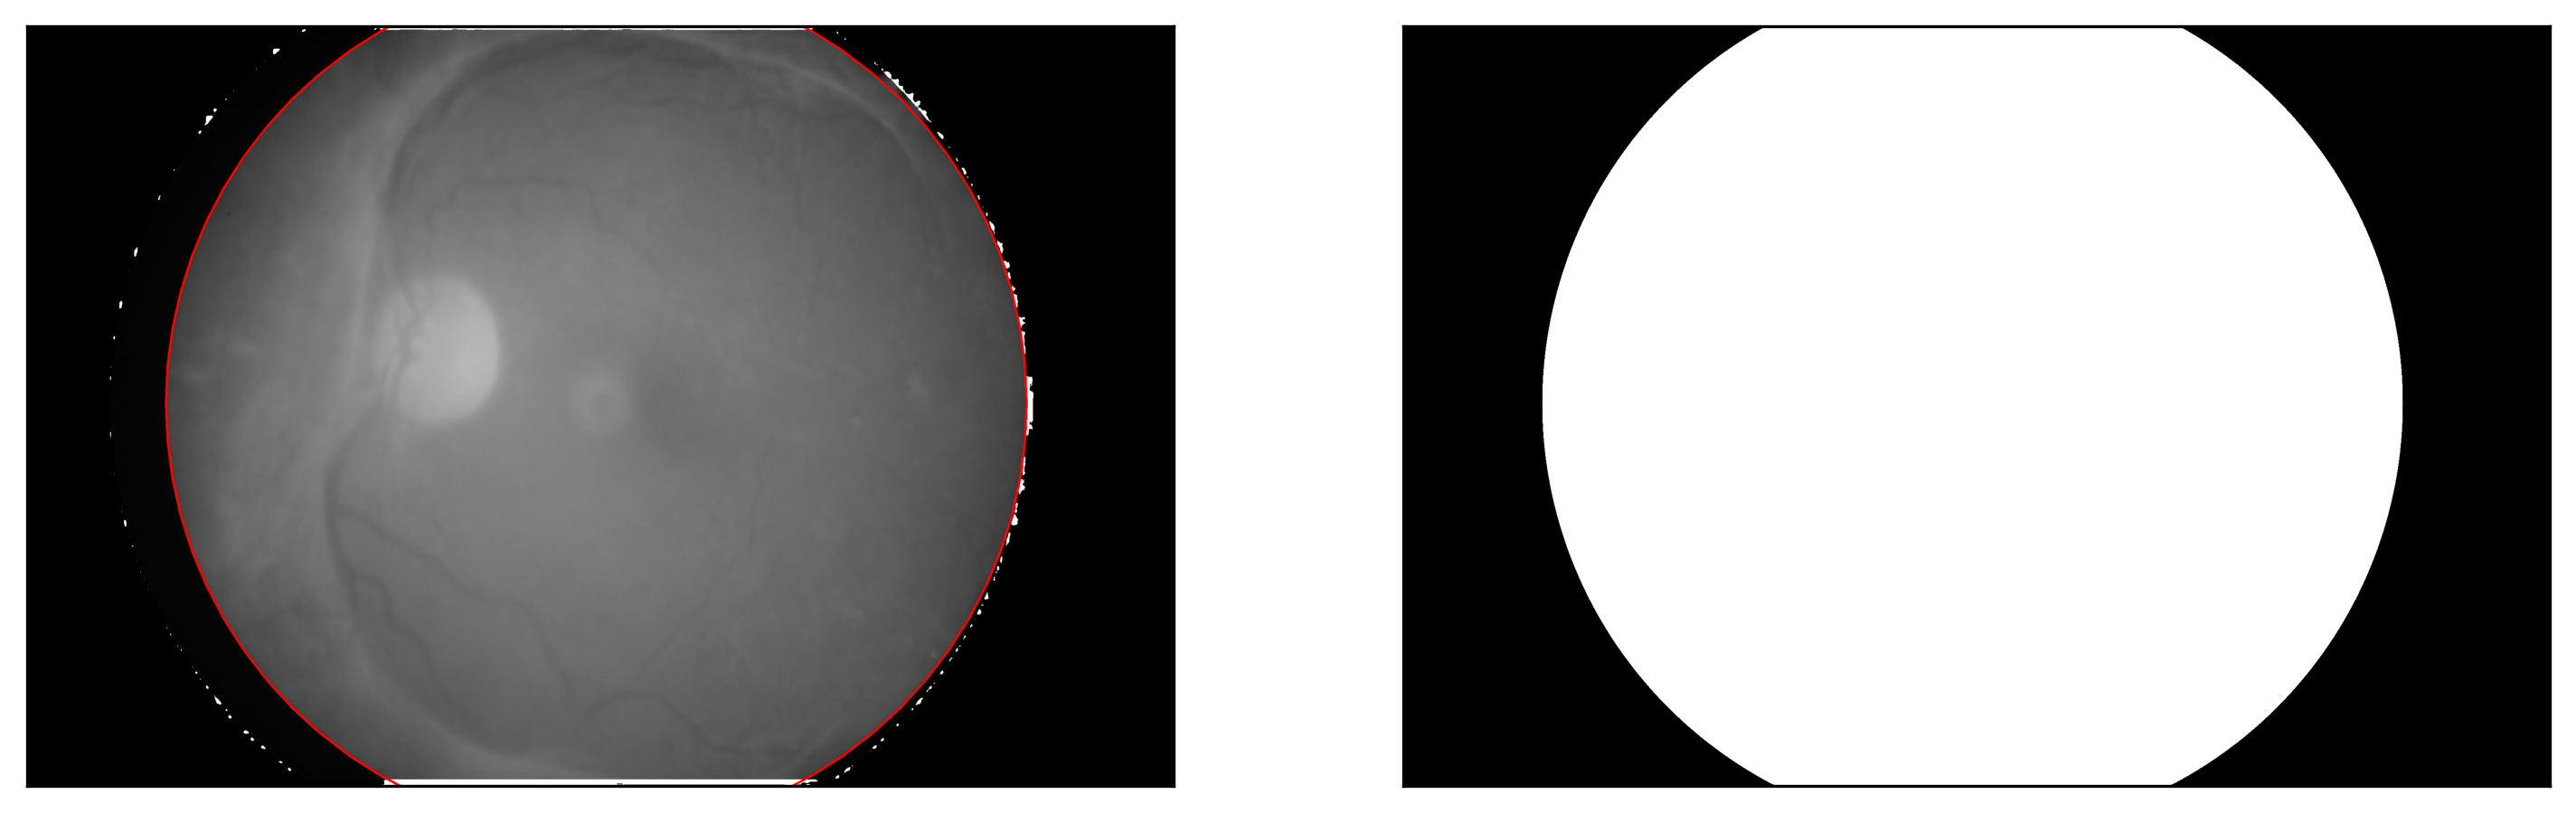
\includegraphics[scale=0.60]{doc_images/circulos_hough.png}
		\caption{A la izquierda, imagen con desenfoque de mediana y círculo detectado (en rojo) mediante la transformada de Hough. A la derecha, máscara binaria generada a partir del círculo.} 
		\label{fig:circulos_hough}
	\end{figure}
\end{center}

Si el método basado en la transformada de Hough no detecta ningún círculo o detecta más de uno, se recurre a un enfoque alternativo basado en la suma de intensidades de los canales de la imagen. Las imágenes de fondo de ojo son a color, por lo que están compuestas por tres canales (rojo, verde y azul), cada uno con valores de intensidad entre 0 (negro) y 255 (blanco). Al sumar las intensidades de los tres canales en cada píxel, se obtiene una imagen en escala de grises que acentúa las diferencias entre las regiones con contenido retiniano (dentro del FOV) y el fondo. Esto resulta útil en casos donde el fondo no es completamente negro, como ocurre con ciertas cámaras que introducen ruido o iluminaciones residuales. De este modo, se mejora el contraste entre el FOV y el resto de la imagen.

Luego, se aplica el umbral de Otsu para determinar un valor de corte que permita separar ambas regiones. Este método analiza el histograma de intensidades de la imagen y selecciona automáticamente un valor de umbral que minimiza la varianza dentro de cada clase y maximiza la varianza entre clases, separando así de forma óptima los píxeles en dos grupos: uno que representa los objetos (en este caso, la retina) y otro el fondo. Se genera una máscara binaria donde los píxeles con valores superiores al umbral se asignan como \textit{True} y el resto como \textit{False}. Finalmente, se realiza un relleno de agujeros\footnote{Para realizar el relleno de agujeros se utiliza la función \textit{binary\_fill\_holes} del módulo ndimage de SciPy. Esta función identifica regiones cerradas dentro de los objetos binarios (representadas por \textit{False} rodeados de \textit{True}) y las completa.} sobre la máscara binaria, garantizando que la región segmentada sea continua y sin interrupciones.

\begin{center}
	\begin{figure}[H]
		\centering
		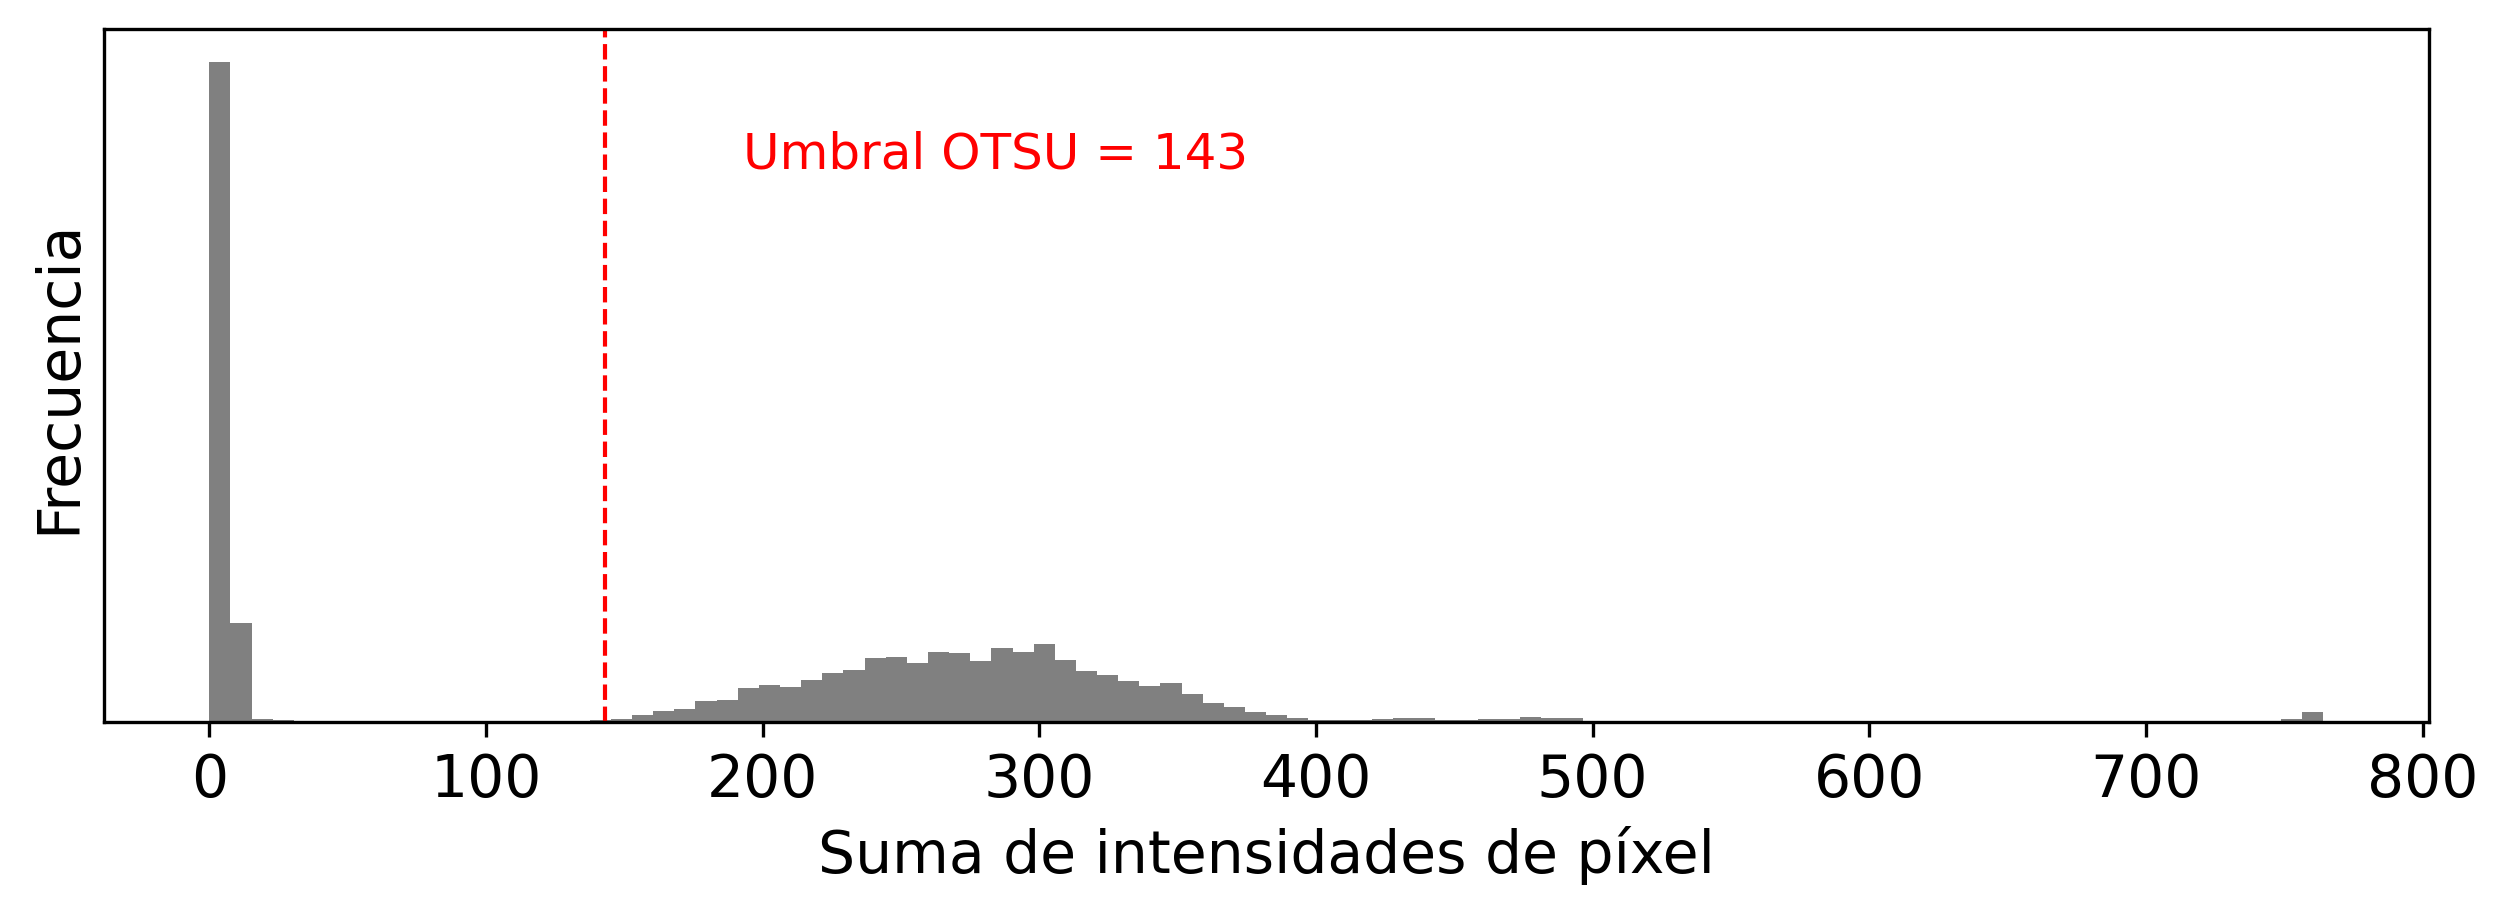
\includegraphics[scale=0.60]{doc_images/histograma_suma.png}
		\caption{Histograma de la suma de intensidades RGB en imágenes donde la transformada de Hough no detectó un único círculo.} 
		\label{fig:histograma_suma}
	\end{figure}
\end{center}

\subsection{Ajuste del tamaño de la imagen}
Una vez obtenida la máscara del campo de visión (FOV), se aplica una función que permite recortar la imagen original, conservando únicamente la región correspondiente al contenido retiniano. En primer lugar, se utiliza la máscara para establecer en negro (intensidad cero) todos los píxeles de la imagen que se encuentran fuera del área delimitada como FOV, eliminando así cualquier información irrelevante o artefactos. Luego, se identifican las coordenadas de un rectángulo (bounding box) que encierra completamente la región marcada como FOV en la máscara binaria. Finalmente, se recorta la imagen utilizando dichas coordenadas, devolviendo únicamente la porción útil.

\subsection{Recorte del Bounding Box}
Para finalizar el preprocesamiento, la imagen segmentada y recortada se redimensiona a un tamaño fijo de 512×512 píxeles\footnote{En este caso se elige un tamaño de 512×512 píxeles, que permite preservar mayor detalle que resoluciones más bajas, sin comprometer demasiado el rendimiento computacional.}. Aunque arquitecturas como ResNet permiten procesar imágenes de distintas dimensiones gracias al uso de adaptive pooling, establecer una resolución estándar facilita el procesamiento en lotes y permite un uso más eficiente de los recursos computacionales.

\section{Normalización de imágenes}
Una vez redimensionadas, se calcula la media y el desvío estándar de los valores de píxel por canal (R, G, B) en el conjunto de entrenamiento. En este caso, los valores obtenidos fueron:

\begin{itemize}
	\item \textbf{Media}: [0.1948, 0.2880, 0.4238]
	\item \textbf{Desvío estandar}: [0.1661, 0.2021, 0.2782]
\end{itemize}

Estos valores se utilizan para normalizar las imágenes, es decir, restar la media y dividir por el desvío en cada canal.

Esta técnica ayuda a estabilizar el entrenamiento: Al quedar los valores normalizados en un rango cercano a -1 y 1, las actualizaciones de los pesos se vuelven más uniformes, evitando saltos muy grandes o avances demasiado pequeños durante la optimización. Además, valores de entrada en escalas similares permiten que el algoritmo de optimización (como el gradiente descendente) converja más rápido, ya que las actualizaciones de los parámetros no se ven afectadas por magnitudes desiguales. Como beneficio adicional, la normalización reduce el riesgo de que ciertas regiones con valores más altos dominen sobre otras, lo que puede dificultar que el modelo aprenda representaciones relevantes. 

\subsection{Data Augmentation}
Antes de entrenar el modelo, se aplican técnicas de data augmentation al conjunto de entrenamiento. Estas técnicas introducen variaciones artificiales en las imágenes (como rotaciones, recortes aleatorios o volteos horizontales), con el objetivo de aumentar la diversidad de los datos y evitar que memorice patrones específicos de los datos de entrenamiento.
En este trabajo se utilizaron tres transformaciones principales sobre las imágenes de entrenamiento:

\begin{itemize}
	\item Volteo horizontal aleatorio (RandomHorizontalFlip): con una probabilidad del 50\%, la imagen se invierte de izquierda a derecha.
	\item Rotación aleatoria (RandomRotation): rota la imagen un ángulo aleatorio entre -15° y 15°, utilizando interpolación bilineal para preservar la calidad de la imagen y rellenando las zonas vacías con negro.
	\item{Volteo vertical aleatorio (RandomVerticalFlip): con una probabilidad del 50\%, la imagen se invierte de arriba hacia abajo.}
\end{itemize}

Es importante destacar que en las imágenes de fondo de ojo no siempre se sigue una orientación estándar: pueden estar centradas en la mácula, en el disco óptico o presentar leves inclinaciones según cómo se haya realizado la captura. Por eso, introducir variaciones como rotaciones y volteos durante el entrenamiento ayuda al modelo a enfocarse en las características relevantes de la imagen, sin depender de la posición exacta de las estructuras anatómicas.

\subsection{Arquitectura}
En este trabajo se utilizó una arquitectura basada en ResNet-18, una red convolucional profunda con conexiones residuales que permiten un entrenamiento más eficiente y estable. La ResNet-18 se compone de bloques residuales que aprenden ajustes sobre la representación existente en lugar de reemplazarla por completo, lo que facilita el flujo de gradientes y evita problemas comunes en redes profundas, como la degradación del rendimiento al aumentar la cantidad de capas.

\begin{center}
	\begin{figure}[H]
		\centering
		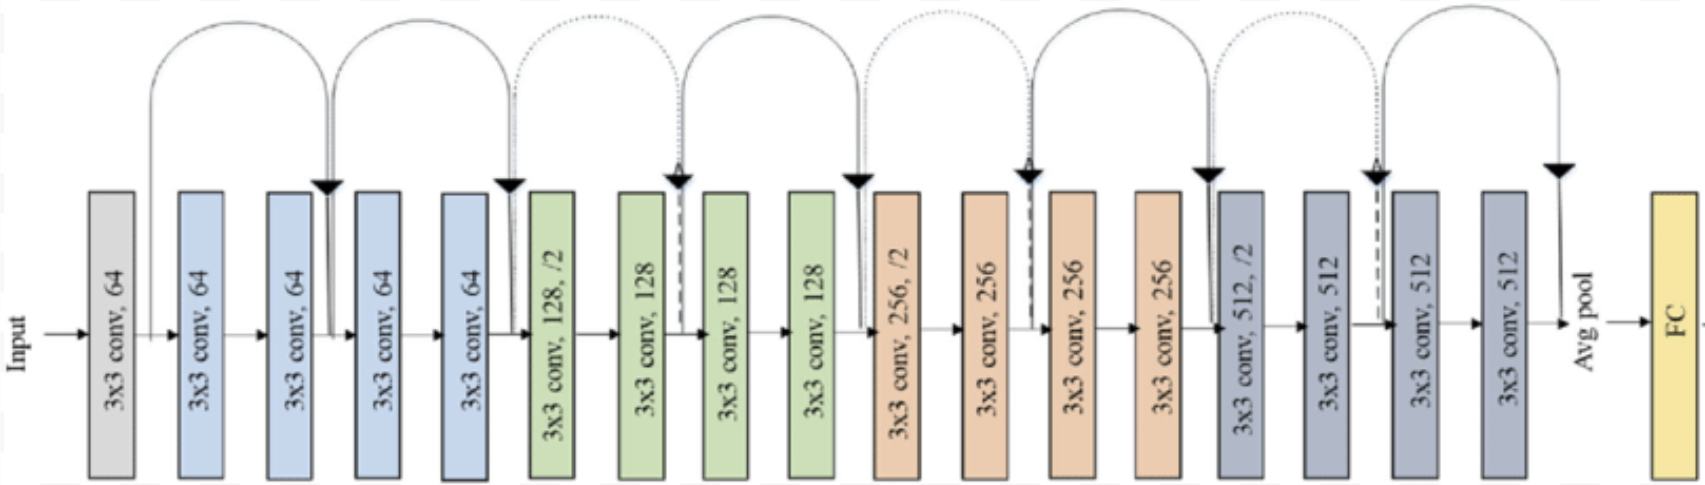
\includegraphics[scale=0.70]{doc_images/resnet18.png}
		\caption{Arquitectura de la red ResNet-18.} 
		\label{fig:resnet18}
	\end{figure}
\end{center}

La arquitectura de ResNet-18 se compone de una capa convolucional inicial, seguida por cuatro etapas residuales compuestas por bloques básicos (BasicBlocks), y una capa final de clasificación. El cuadro \ref{tab:resnet18} resume las principales características de cada etapa de la red.


\begin{table}[H]
	\centering
	\renewcommand{\arraystretch}{1.5}
	\resizebox{\textwidth}{!}{
		\begin{tabular}{ ||c|c||  }
			\hline
			\hline
			\textbf{Etapa} & \textbf{Descripción} \\
			\hline
			\hline
			\cellcolor[HTML]{d6d1d1} \textbf{Capa Inicial} & 
			\makecell[l]{- Conv2d (7×7, stride 2, padding 3)\\
				- BatchNorm \\
				- ReLU \\
				- MaxPooling (3x3, stride 2)} \\		
			\hline
			\hline
			\cellcolor[HTML]{abd6f7} \textbf{Etapa residual 1} & - 2 x BasicBlock con 64 filtros, stride 1 \\		
			\hline
			\hline
			\cellcolor[HTML]{a9dda2} \textbf{Etapa residual 2} & - 2 x BasicBlock con 128 filtros, el primero con stride 2 \\		
			\hline
			\hline
			\cellcolor[HTML]{ffb980} \textbf{Etapa residual 3} & - 2 x BasicBlock con 256 filtros, el primero con stride 2 \\		
			\hline
			\hline
			\cellcolor[HTML]{9ab2c1} \textbf{Etapa residual 4} & - 2 x BasicBlock con 512 filtros, el primero con stride 2 \\		
			\hline
			\hline
			\cellcolor[HTML]{fbdc89} \textbf{Capa Final} & 
			\makecell[l]{- Global Average Pooling \\
				- Capa totalmente conectada (2 salidas: buena o mala calidad)} \\
			\hline
		\end{tabular}
	}
	\caption{Componentes principales de la arquitectura ResNet-18.}
	\label{tab:resnet18}
\end{table}


Cada una de las etapas residuales mencionadas se compone de dos BasicBlocks, cuya estructura se detalla a continuación:
\begin{itemize}
	\item Conv2d (3x3)
	\item BatchNorm
	\item ReLU
	\item Conv2d (3x3)
	\item BatchNorm
	\item Suma residual: \textit{F(x) + x}
\end{itemize}

\begin{center}
	\begin{figure}[H]
		\centering
		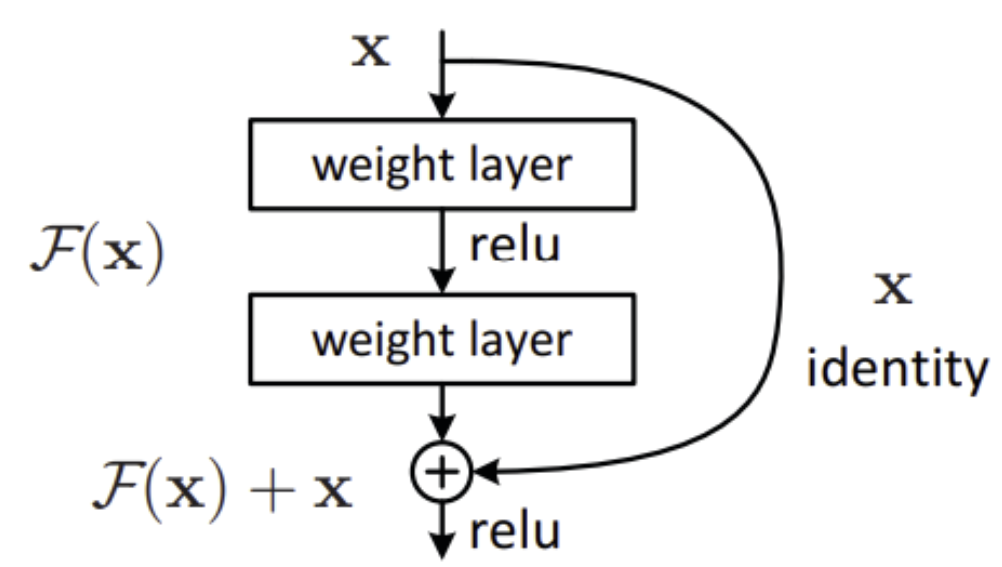
\includegraphics[scale=0.70]{doc_images/residual.png}
		\caption{Estructura de un bloque residual (BasicBlock). La entrada “x” se bifurca en dos caminos: uno donde se aplican dos capas convolucionales y otro que preserva la señal original con una conexión identidad. Finalmente, ambas salidas se suman y se aplica una función de activación ReLU \parencites{he2015deep}.} 
		\label{fig:residual}
	\end{figure}
\end{center}

En una red sin conexiones residuales, cada capa debe aprender directamente la transformación completa que mapea una entrada a una salida deseada. Esto implica que, si una capa no logra detectar patrones relevantes, por ejemplo, si una capa intermedia genera activaciones nulas o muy bajas, las siguientes capas se ven forzadas a operar sobre representaciones poco informativas, comprometiendo la capacidad de aprendizaje del modelo. Además, a medida que aumenta la profundidad de la red, puede intensificarse el problema del desvanecimiento del gradiente\footnote{El desvanecimiento del gradiente es un problema que ocurre en redes neuronales profundas cuando los gradientes que se propagan hacia las capas iniciales se vuelven extremadamente pequeños. Durante la retropropagación del error, los gradientes se multiplican sucesivamente mediante la regla de la cadena. Si las derivadas de las funciones de activación son pequeñas, esto provoca que los gradientes se reduzcan exponencialmente a medida que se avanza hacia las capas cercanas a la entrada, impidiendo que reciban actualizaciones significativas y dificultando el entrenamiento de la red.}, dificultando la retropropagación efectiva del error hacia las capas iniciales.

Las conexiones residuales mitigan ambos problemas: facilitan la propagación directa de la información útil a través de la red y simplifican la optimización, ya que el modelo aprende únicamente la diferencia entre la entrada y la salida deseada. Esto mejora tanto la precisión como la eficiencia del entrenamiento.

La arquitectura ResNet-18 fue seleccionada por ser una de las más utilizadas en investigaciones de visión computacional, especialmente en contextos de transferencia de aprendizaje. Su popularidad se debe a una combinación de factores: ofrece una buena capacidad de representación con una profundidad moderada que facilita el entrenamiento, es robusta frente a distintas tareas, y puede adaptarse a imágenes de entrada de diferentes tamaños sin requerir preprocesamiento estricto. Además, su disponibilidad como modelo preentrenado en conjuntos de datos grandes como ImageNet permite reutilizar conocimientos previamente aprendidos y adaptarlos eficazmente a nuevos dominios con datos limitados, como en el caso de este trabajo. Diversos estudios han demostrado que ResNet-18 puede lograr buenos resultados en aplicaciones médicas específicas, incluso cuando se dispone de un conjunto de datos reducido \parencites{kim2022transfer}.


\section{Entrenamiento utilizando transfer learning}
En la práctica, entrenar una red convolucional desde cero no es habitual, ya que esto requiere conjuntos de datos muy grandes para lograr un buen resultado. Por este motivo, una estrategia común consiste en utilizar redes previamente entrenadas en bases de datos extensas, como ImageNet, que contiene más de un millón de imágenes clasificadas en mil categorías. Esta estrategia, conocida como transfer learning, permite aprovechar los conocimientos adquiridos por la red en tareas generales y adaptarlos a un nuevo problema con menos datos disponibles. Existen dos enfoques principales: el uso de la red como extractor de características (feature extraction), donde se aprovechan las representaciones internas aprendidas sin modificar sus pesos, y el fine-tuning, que implica ajustar los pesos de la red preentrenada, total o parcialmente, en función del nuevo conjunto de datos \parencites{cs231n2023transfer}. Como señala \cite{stevens2020deep}, esta última estrategia combina lo mejor de dos mundos: reutiliza características previamente aprendidas por otra red en una tarea diferente (en lugar de diseñarlas manualmente, como se hacía antes del aprendizaje profundo), y al mismo tiempo permite adaptarlas a las particularidades del nuevo problema mediante entrenamiento adicional.

En este trabajo se utilizó una estrategia de fine-tuning a partir de una red ResNet-18 preentrenada en ImageNet. Inicialmente, se reemplazó la capa de clasificación original de la red por una nueva capa adaptada a la tarea específica de clasificación de calidad de imagen. En una primera etapa, se entrenó únicamente esta nueva capa, manteniendo congelados los pesos del resto de la red. Luego, se descongelaron las capas más profundas para continuar el entrenamiento y permitir que el modelo ajustara parcialmente sus representaciones a las características propias del nuevo dominio. Esta decisión se basa en la noción de que las primeras capas de una red convolucional suelen capturar características visuales de bajo nivel, como bordes, texturas y formas simples, que tienden a ser comunes a una gran variedad de imágenes \parencites{stevens2020deep}. Por lo tanto, mantenerlas congeladas ayuda a preservar ese conocimiento general y reduce el riesgo de sobreajuste.

Las estrategias exploradas incluyeron desde el entrenamiento exclusivo de la capa final, manteniendo congeladas el resto de las capas, hasta el fine-tuning progresivo de bloques más profundos de la red, con el objetivo de evaluar el impacto de permitir el ajuste de representaciones internas más complejas. En todos los casos, se utilizaron técnicas estándar de entrenamiento tales como el uso de data augmentation, optimización con Stochastic Gradient Descent (SGD) o Adam (Adaptive Moment Estimation), programación del learning rate mediante scheduler, y entrenamiento con precisión mixta (Automatic Mixed Precision, AMP\footnote{Automatic Mixed Precision: método de Pytorch que permite usar dos tipos de precisión, float16 solo en operaciones que no necesitan tanta precisión, como multiplicaciones de matrices, mientras que,
	algunas operaciones críticas (como la suma de gradientes) siguen en float32 para evitar errores numéricos. \url{https://pytorch.org/tutorials/recipes/recipes/amp_recipe.html}}) para optimizar el uso de la GPU y un tamaño de batch de 128.
	
Las figuras \ref{fig:filtrosConv1}, \ref{fig:actConv1}, \ref{fig:actLayer1}, \ref{fig:actLayer2}, \ref{fig:actLayer3}, \ref{fig:actLayer4} del anexo muestran las características de bajo nivel capturadas por la capa inicial de la ResNet-18 (filtros de bordes y texturas) y el comportamiento interno de sus capas más profundas (mapas de activación de cada bloque).

\section{Función de pérdida}
Para la tarea de clasificación binaria se utilizó la función de pérdida de entropía cruzada (Cross Entropy Loss\footnote{\url{https://pytorch.org/docs/stable/generated/torch.nn.CrossEntropyLoss.html}}), ampliamente empleada en problemas de clasificación supervisada. Esta función mide la discrepancia entre la distribución de probabilidad predicha por el modelo y la verdadera etiqueta de clase, penalizando con mayor severidad aquellas predicciones erróneas en las que el modelo está muy confiado. Cuando el modelo asigna una probabilidad alta a la clase equivocada, el logaritmo de dicha probabilidad es cercano a cero y su negativo produce un valor alto, lo que se traduce en una penalización significativa. Por el contrario, si la probabilidad de la clase equivocada es baja, la penalización será menor. Gracias a esto, el modelo aprende a no “confiar ciegamente” en predicciones incorrectas.

\section{Optimizadores}
Durante el entrenamiento de una red neuronal, el objetivo es encontrar los valores óptimos de los pesos que minimicen una función de pérdida. Para ello, se utilizan algoritmos de optimización basados en el cálculo del gradiente, que actualizan los pesos del modelo en función del error cometido. El más utilizado de estos algoritmos es el descenso del gradiente (GD).

El descenso del gradiente es un método iterativo que busca minimizar una función de pérdida calculando las derivadas parciales de dicha función con respecto a cada uno de los parámetros del modelo. Este conjunto de derivadas forma el gradiente e indica la dirección en la que la función crece más rápidamente. Por lo tanto, la actualización de los pesos se realiza en la dirección contraria, es decir, hacia el mínimo. La magnitud del paso de actualización está determinada por un hiperparámetro conocido como tasa de aprendizaje (learning rate).

La actualización de cada parámetro  se realiza según la siguiente regla:

\[
\Delta w \;=\; -\,\eta\,\frac{\partial L}{\partial w} \quad\Longrightarrow\quad
w \leftarrow w + \Delta w
\]

donde:
\begin{itemize}
	\item $\Delta w$ w es el cambio aplicado al parámetro.
	\item $\eta$ es la tasa de aprendizaje.
	\item $\frac{\partial L}{\partial w}$ es la derivada parcial de la función de pérdida respecto a $w$.
\end{itemize}

El método clásico de descenso del gradiente se calcula utilizando todos los ejemplos del conjunto de entrenamiento, lo cual resulta computacionalmente costoso y lento, especialmente con grandes volúmenes de datos. En este trabajo se utilizó una variante de este método, el Stochastic Gradient Descent (SGD), que actualiza los pesos del modelo utilizando pequeños lotes de datos (mini-batches) en lugar de todo el conjunto de entrenamiento. Este enfoque, aunque introduce ciertas aproximaciones imprecisas, favorece la convergencia del modelo y evita que el proceso de optimización se quede atrapado en mínimos locales \parencites{stevens2020deep}. Para mejorar la estabilidad y acelerar la convergencia, se utilizó la técnica de momentum, que en lugar de solo mirar el gradiente actual para actualizar los pesos, el optimizador también tiene en cuenta la dirección anterior en la que venía actualizando.

Además del algoritmo SGD, en este trabajo se utilizó Adam (Adaptive Moment Estimation), un optimizador que incorpora promedios móviles de los gradientes y sus cuadrados. Esta estrategia permite ajustar de manera adaptativa la tasa de aprendizaje de cada parámetro, facilitando una convergencia más rápida y estable.

En cada iteración, Adam mantiene y actualiza dos promedios móviles:

\[
m_t \;=\; \beta_1 \cdot m_{t-1} + (1 - \beta_1) \cdot g_t
\]

\[
v_t \;=\; \beta_2 \cdot v_{t-1} + (1 - \beta_2) \cdot g_t^2
\]

donde $g_t$ es el gradiente en el paso $t, \beta_1, \beta_2$ son coeficientes de decaimiento.

Para evitar sesgos en los primeros pasos, se aplican correcciones:

\[
\widehat{m_t} \;=\; \frac{m_t}{(1 - \beta_1^t)} \,,\, \widehat{v_t} \;=\; \frac{v_t}{(1 - \beta_2^t)}
\]

Finalmente, los parámetros se actualizan mediante:

\[
w_{t+1} \;=\; w_t - \eta \cdot \frac{\widehat{m_t}}{\sqrt{\widehat{v_t}} + \epsilon}
\]

Esta actualización permite que se ajuste automáticamente la magnitud del paso para cada parámetro individual, según la historia reciente de los gradientes.

Sin embargo, en este trabajo se utilizó específicamente AdamW, una variante de Adam que mejora el tratamiento de la regularización L2. A diferencia de Adam, que incluye el término de regularización dentro del cálculo del gradiente adaptativo, AdamW separa explícitamente ese término (también conocido como weight decay). Esta separación permite controlar de forma más precisa el efecto de la regularización sobre los pesos del modelo, lo cual contribuye a una mejor generalización \parencites{loshchilov2019decoupled}.

La actualización de los parámetros en AdamW se realiza de la siguiente manera:

\[
w_{t+1} \;=\; w_t - \eta \cdot (\frac{\widehat{m_t}}{\sqrt{\widehat{v_t}} + \epsilon} + \lambda \cdot w_t)
\]

donde $\lambda \cdot w_t$ es el término de penalización L2 aplicado directamente sobre los pesos y no sobre el gradiente.

\section{Learning rate schedulers}
Durante el entrenamiento, además del algoritmo de optimización, se utilizaron planificadores de tasa de aprendizaje (schedulers) con el objetivo de mejorar la convergencia del modelo y evitar estancamientos en mínimos locales. Estos mecanismos ajustan la tasa de aprendizaje de forma dinámica a lo largo de las épocas, según estrategias predefinidas.

Se exploraron tres tipos distintos de schedulers:

\begin{itemize}
	\item StepLR: reduce la tasa de aprendizaje de manera escalonada, disminuyéndola por un factor constante cada cierta cantidad de épocas. Esta estrategia es útil cuando se espera que el modelo se beneficie de una menor tasa de aprendizaje en etapas avanzadas del entrenamiento.
	\item ReduceLROnPlateau: ajusta la tasa de aprendizaje cuando una métrica de evaluación deja de mejorar. Esta estrategia permite que la tasa de aprendizaje se reduzca de forma reactiva ante una meseta en el rendimiento del modelo, favoreciendo una optimización más precisa.
	\item CosineAnnealingLR: aplica una reducción de la tasa de aprendizaje siguiendo una función coseno decreciente. Esta estrategia permite comenzar con una tasa alta para una exploración más amplia del espacio de parámetros y luego reducirla suavemente hacia el final del entrenamiento, promoviendo una convergencia más fina.
\end{itemize}

\section{Resultados}
A continuación, se detallan las estrategias evaluadas, junto con los resultados obtenidos en términos de pérdida y precisión sobre el conjunto de validación.

\begin{table}[H]
	\centering
	\renewcommand{\arraystretch}{2}
	\resizebox{\textwidth}{!}{
		\begin{tabular}{ ||c|c|c|c|c|c|c||  }
			\hline
			\textbf{Estrategia} & \textbf{Optimizador} & \textbf{LR} & \textbf{Scheduler} & \textbf{Momentum} & \textbf{Tiempo (minutos)} & \textbf{Best Acc. Validation} \\
			\hline
			Modelo base (solo FC) & SGD & 0.001 & StepLR(step\_size=7, γ=0.1) & 0.90 & 610.4 & 0.9777 \\
			\hline
			\textcolor{red}{\textbf{Capa 4}} + FC & SGD & 0.001 & StepLR(step\_size=7, γ=0.1) & 0.90 & 598.3 & 0.9790 \\
			\hline
			\hline
			Capa 4 + FC & SGD & \textcolor{red}{\textbf{0.005}} & StepLR(step\_size=7, γ=0.1) & 0.90 & 613.4 & 0.9822 \\
			\hline
			Capa 4 + FC & SGD & \textcolor{red}{\textbf{0.0005}} & StepLR(step\_size=7, γ=0.1) & 0.90 & 538.9 & 0.9776 \\
			\hline
			\hline
			Capa 4 + FC & SGD & 0.001 & \textcolor{red}{\textbf{\makecell{ReduceLROnPlateau\\(factor=0.1, p=3,mode=”max”)}}} & 0.90 & 538.9 & 0.9810 \\
			\hline
			Capa 4 + FC & SGD & 0.001 & \textcolor{red}{\textbf{\makecell{CosineAnnealingLR\\(T\_max=25)}}} & 0.90 & 782.3 & 0.9812 \\
			\hline
			\hline
			Capa 4 + FC & SGD & 0.001 & StepLR(step\_size=7, γ=0.1) & \textcolor{red}{\textbf{0.95}} & 552.9 & 0.9809 \\
			\hline
			Capa 4 + FC & SGD & 0.001 & StepLR(step\_size=7, γ=0.1) & \textcolor{red}{\textbf{0.85}} & 552.9 & 0.9793 \\
			\hline
			\hline
			Capa 4 + FC & \textcolor{red}{\textbf{AdamW}} & 0.001 & StepLR(step\_size=7, γ=0.1) & 0.90 & 552.4 & 0.9839 \\
			\hline
			Capa 4 + FC & \textcolor{red}{\textbf{AdamW}} & 0.001 &  \textcolor{red}{\textbf{\makecell{ReduceLROnPlateau\\(factor=0.1, p=3,mode=”min”)}}}  & 0.90 & 595.7 & 0.9866 \\
			\hline
			\hline
			\makecell{\textcolor{red}{\textbf{Capa 3}} +\\ Capa 4 + FC} & SGD & 0.001 &  StepLR(step\_size=7, γ=0.1)  & 0.90 & 552.7 & 0.9807 \\
			\hline
			\makecell{\textcolor{red}{\textbf{Capa 3}} +\\ Capa 4 + FC} & SGD & 
			\textcolor{red}{\textbf{\makecell{Capa 3 = 0.0001\\ Capa 4 = 0.0001\\ FC = 0.001}}} &  StepLR(step\_size=7, γ=0.1)  & 0.90 & 608.4 & 0.9782 \\
			\hline
			\makecell{\textcolor{red}{\textbf{Capa 3}} +\\ Capa 4 + FC} & SGD & 
			\makecell{Capa 3 = 0.0001\\ \textcolor{red}{\textbf{Capa 4 = 0.0005}} \\ FC = 0.001} &  StepLR(step\_size=7, γ=0.1)  & 0.90 & 552.8 & 0.9791 \\
			\hline
			\makecell{\textcolor{red}{\textbf{Capa 3}} +\\ Capa 4 + FC} & SGD & 
			\textcolor{red}{\textbf{0.005}} &  StepLR(step\_size=7, γ=0.1)  & \textcolor{red}{\textbf{0.95}} & 655.5 & 0.9856 \\
			\hline
			\makecell{\textcolor{red}{\textbf{Capa 3}} +\\ Capa 4 + FC} & SGD & 
			\makecell{\textcolor{red}{\textbf{Capa 3 = 0.001}} \\ Capa 4 = 0.005 \\ FC = 0.005} &  StepLR(step\_size=7, γ=0.1)  &  \textcolor{red}{\textbf{0.95}} & 654.3 & 0.9850 \\
			\hline
		\end{tabular}
)	}
	\caption{Resumen de pruebas de entrenamiento.}
	\label{tab:estrategias}
\end{table}

\begin{center}
	\begin{figure}[H]
		\centering
		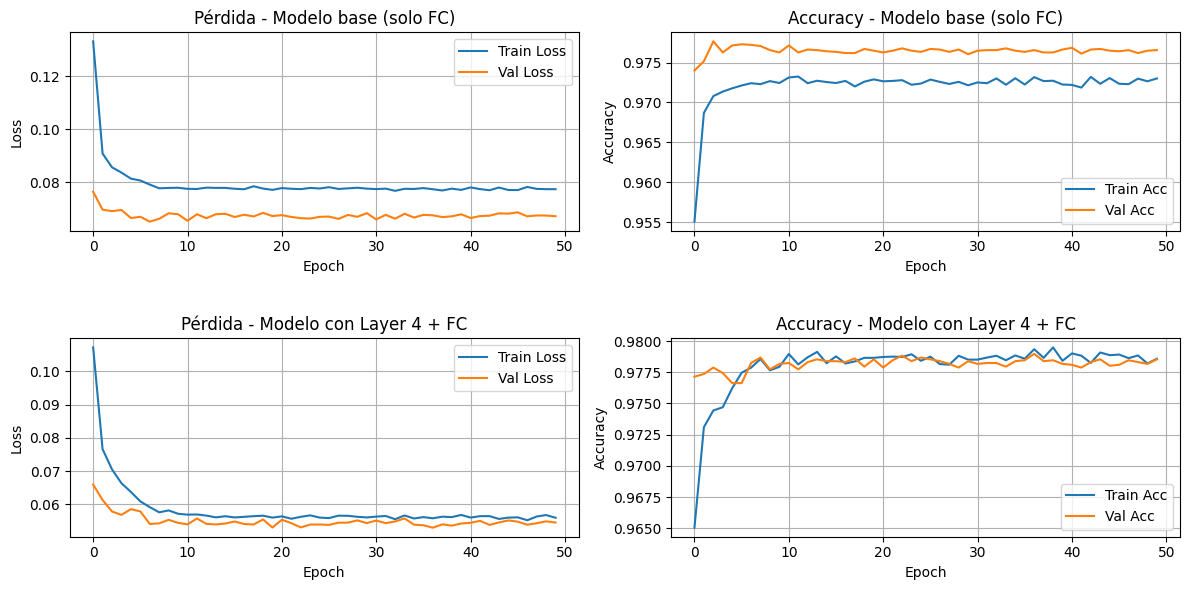
\includegraphics[scale=0.45]{doc_images/baseline.png}
		\caption{Modelos base. Curvas de pérdida (loss) y exactitud (accuracy) por época para dos configuraciones: un modelo que entrena solo la capa fully connected sobre una red base preentrenada congelada, y otro que también entrena la cuarta capa de dicha red.} 
		\label{fig:baseline}
	\end{figure}
\end{center}

\begin{center}
	\begin{figure}[H]
		\centering
		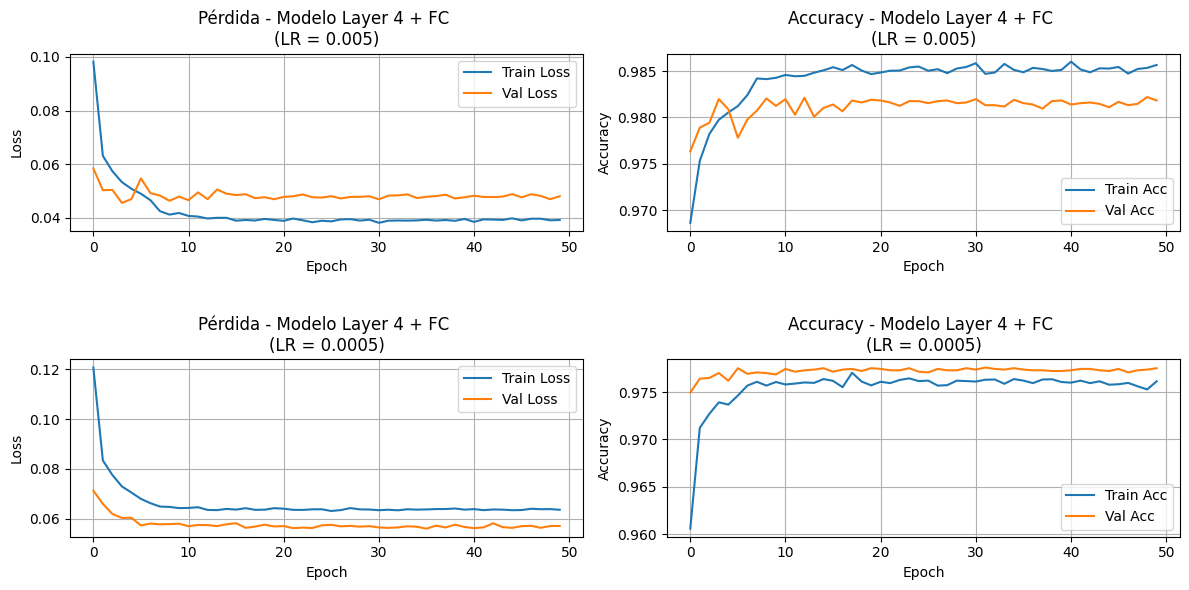
\includegraphics[scale=0.45]{doc_images/lr.png}
		\caption{Variación de tasa de aprendizaje. Curvas de pérdida (loss) y exactitud (accuracy) por época para dos configuraciones de tasa de aprendizaje: una con una tasa de 0.005 y otra con una tasa de 0.0005.} 
		\label{fig:lr}
	\end{figure}
\end{center}

\begin{center}
	\begin{figure}[H]
		\centering
		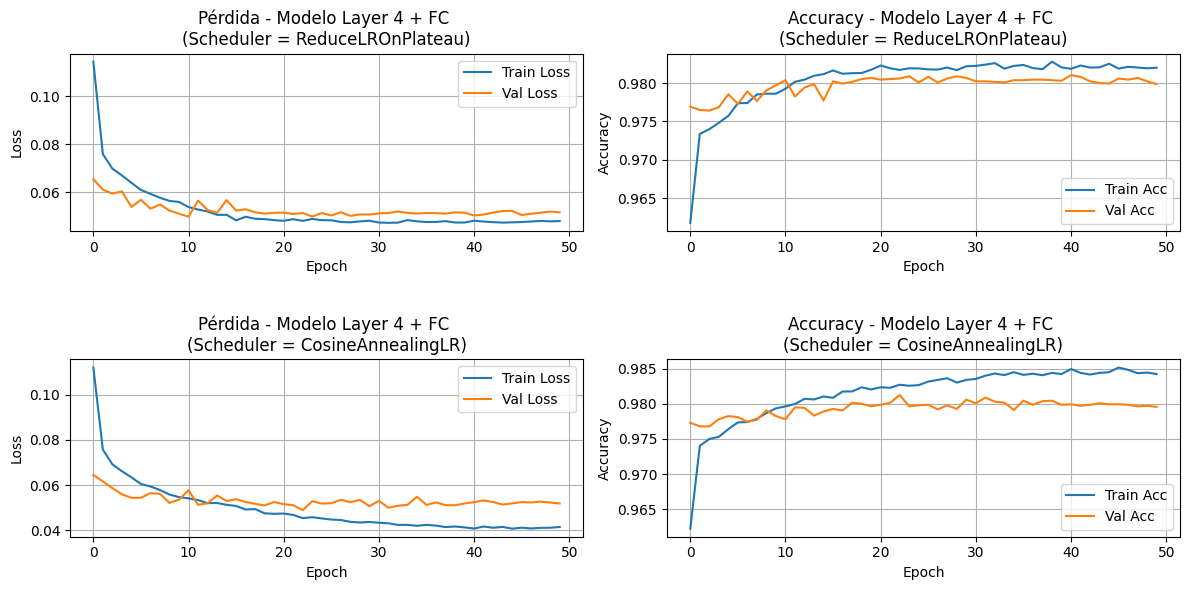
\includegraphics[scale=0.45]{doc_images/scheduler.png}
		\caption{Efecto de los schedulers. Curvas de pérdida (loss) y exactitud (accuracy) por época utilizando dos estrategias de programación de tasa de aprendizaje: ReduceLROnPlateau y CosineAnnealingLR.} 
		\label{fig:scheduler}
	\end{figure}
\end{center}

\begin{center}
	\begin{figure}[H]
		\centering
		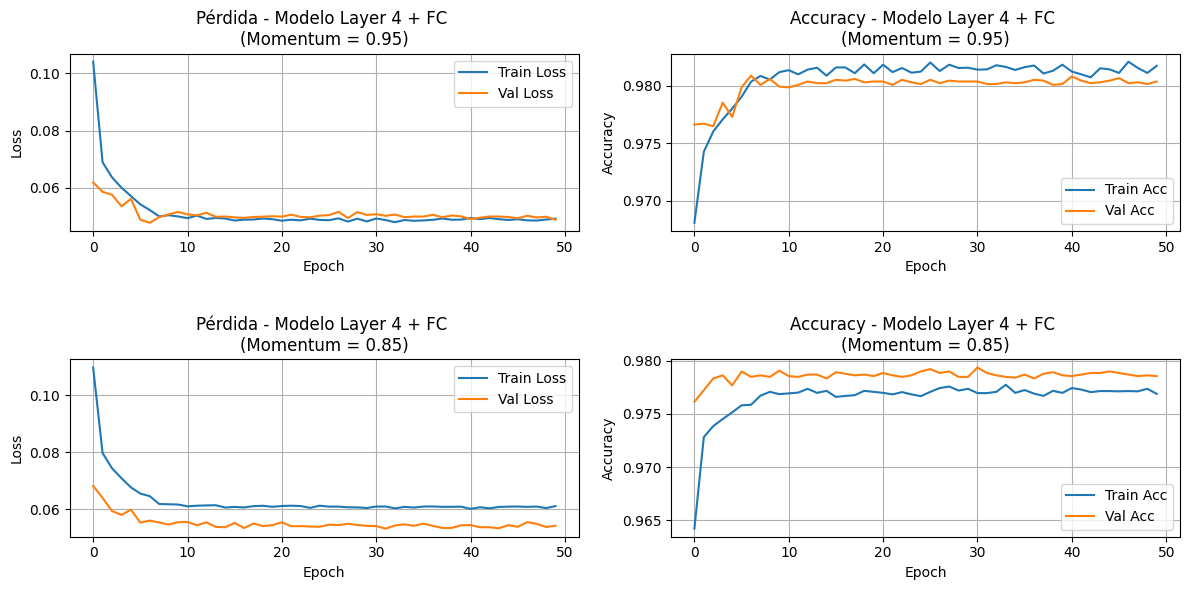
\includegraphics[scale=0.45]{doc_images/momentum.png}
		\caption{Efecto del Momentum. Curvas de pérdida (loss) y exactitud (accuracy) por época utilizando dos valores de momentum: 0.95 y 0.85.} 
		\label{fig:momentum}
	\end{figure}
\end{center}

\begin{center}
	\begin{figure}[H]
		\centering
		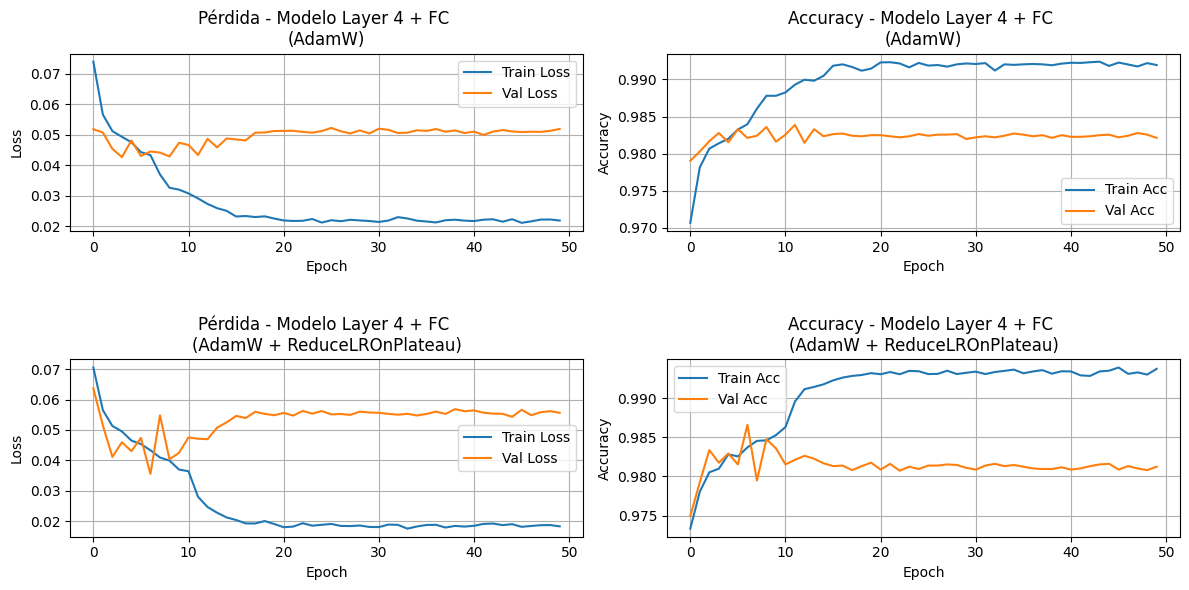
\includegraphics[scale=0.45]{doc_images/adam.png}
		\caption{Optimizador AdamW. Curvas de pérdida (loss) y exactitud (accuracy) por época para dos configuraciones basadas en AdamW: una utilizando únicamente AdamW, y otra combinada con ReduceLROnPlateau.} 
		\label{fig:adam}
	\end{figure}
\end{center}

\begin{center}
	\begin{figure}[H]
		\centering
		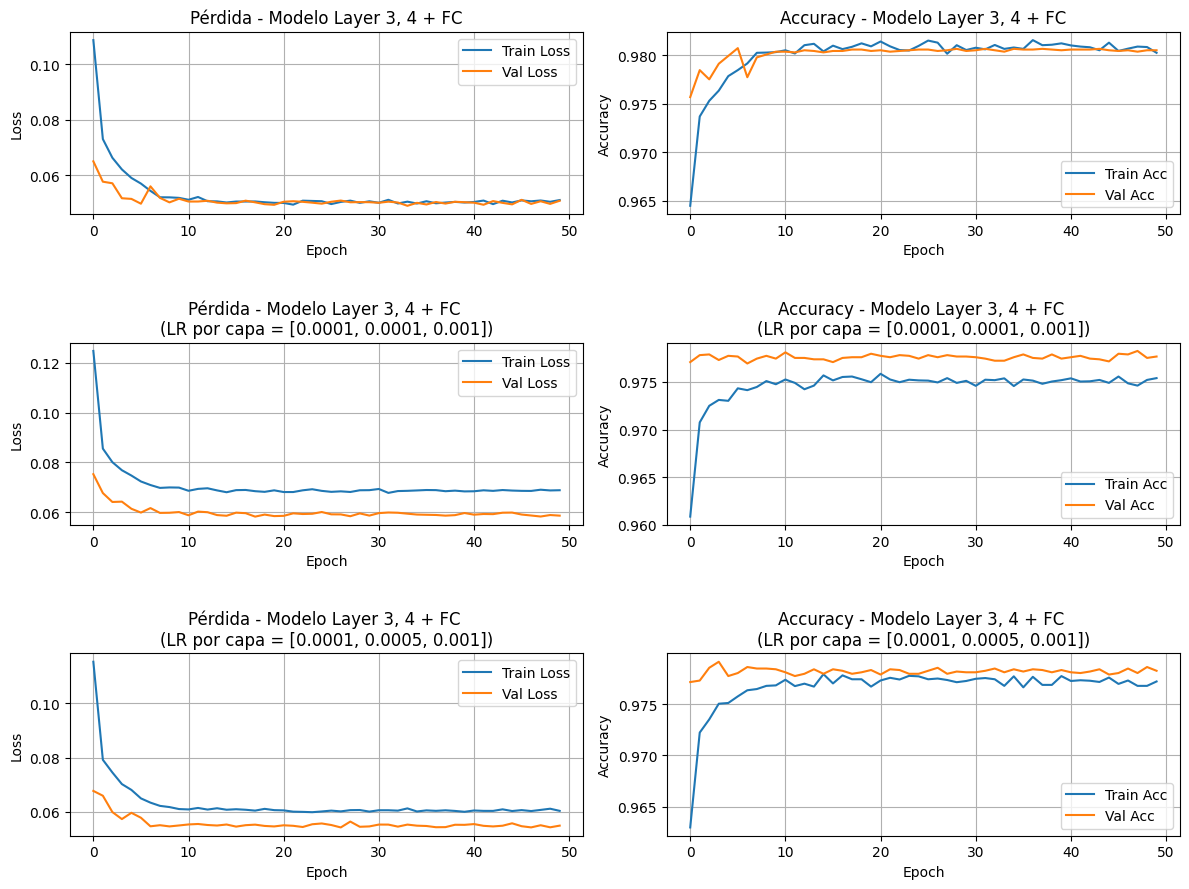
\includegraphics[scale=0.45]{doc_images/layer3.png}
		\caption{Descongelamiento de la capa 3. Curvas de pérdida y exactitud por época para tres configuraciones de fine-tuning de las capas 3 y 4 con distintas tasas de aprendizaje.} 
		\label{fig:layer3}
	\end{figure}
\end{center}

\begin{center}
	\begin{figure}[H]
		\centering
		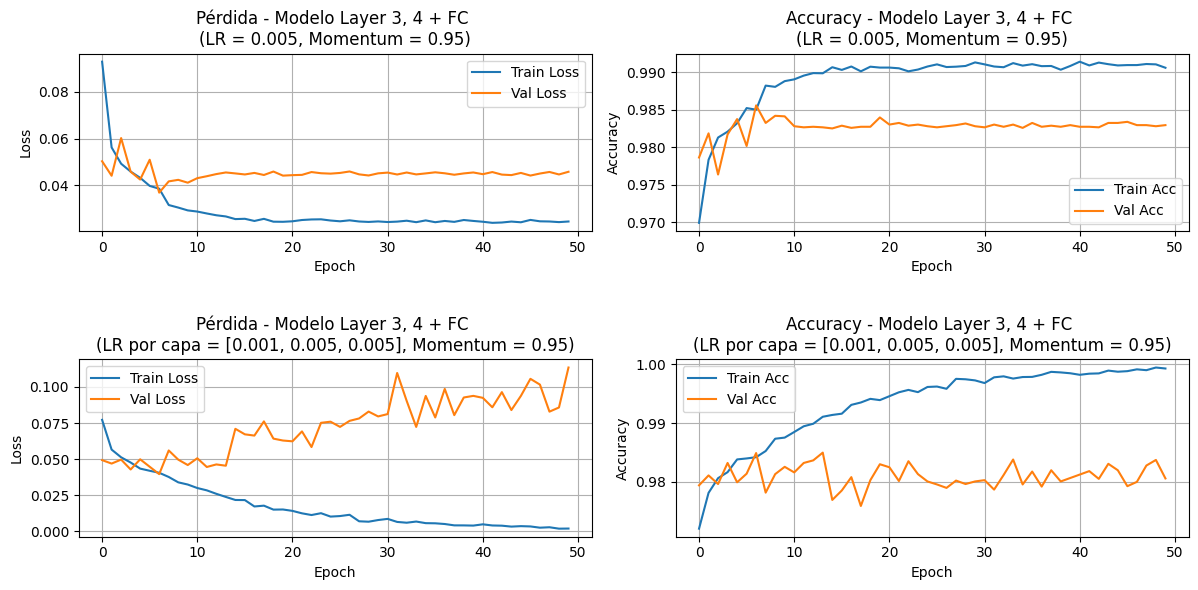
\includegraphics[scale=0.45]{doc_images/ultimas.png}
		\caption{Combinaciones de hiperparámetros. Curvas de pérdida y exactitud por época para dos configuraciones avanzadas de hiperparámetros: una combinando LR alta (0.005) con momentum 0.95, y otra empleando tasas de aprendizaje diferenciadas por capa ([0.001, 0.005, 0.005]) junto con momentum 0.95.} 
		\label{fig:ultimas}
	\end{figure}
\end{center}

La primera prueba, en la que se entrena únicamente la capa totalmente conectada (FC), ya muestra resultados positivos, lo que destaca el poder del transfer learning. A pesar de haber sido preentrenado en un conjunto de datos muy diferente al de imágenes de fondo de ojo, el modelo logra capturar representaciones que resultan útiles para esta nueva tarea. Esto demuestra que incluso con un ajuste mínimo, es posible obtener un desempeño aceptable, gracias a que las características aprendidas previamente son lo suficientemente generales como para transferirse a otros dominios.

Al permitir además el entrenamiento de la capa 4 (segunda prueba), se observa una mejora en el desempeño del modelo junto con una mejor capacidad de generalización (menor diferencia entre train y val). Esta mejora sugiere que, si bien las representaciones generales ya aportan una base sólida, afinar capas más profundas permite una mejor adaptación a las características específicas del nuevo conjunto de datos.

Las pruebas con diferentes tasas de aprendizaje muestran que, al darle mayor sinergia al proceso de aprendizaje, la loss converge más rápido y hay una mejora en el accuracy, pero también comienza a observarse algo de overfitting en los datos de entrenamiento.

En cuanto a los diferentes schedulers, tanto ReduceLROnPlateau como CosineAnnealingLR alcanzan valores similares de accuracy, aunque el segundo requiere más tiempo para completar el entrenamiento. Ninguno de los dos mejora el accuracy obtenido con un aumento de la learning rate. Sin embargo, a favor de ReduceLROnPlateau, se puede destacar que su comportamiento de convergencia es más suave y ayuda a reducir la diferencia entre las curvas de entrenamiento y validación, lo que indica una mejor capacidad de generalización.

La diferencia en el momentum de los modelos con SGD no mostró un impacto tan significativo como el logrado con el optimizador AdamW, el cual no solo mejora el accuracy, sino que, al combinarse con ReduceLROnPlateau, también mostró una convergencia más rápida y una tasa de error más baja en comparación con SGD.

Descongelar la capa 3 con distintas configuraciones de hiperparámetros no superó el rendimiento del modelo optimizado con AdamW, lo que sugiere que los mapas de características preentrenados en capas más profundas ya aportan la información necesaria para la tarea.

El modelo entrenado con AdamW y ReduceLROnPlateau alcanzó la mayor precisión de validación (98.66\% en la época 7), superando al resto de configuraciones. Aunque a partir de la época 10 muestra un incremento en la brecha entre entrenamiento y validación, indicativo de sobreajuste, su capacidad de converger rápidamente y el ajuste automático de la tasa de aprendizaje permiten aplicar early stopping en el punto óptimo. Por ello, y dado que el principal objetivo es maximizar la precisión en validación, el modelo final seleccionado para la fase de evaluación fue AdamW + ReduceLROnPlateau.

\section{Evaluación}
El cuadro \ref{tab:evaluacion} resume las métricas de desempeño obtenidas por el modelo final al ser evaluado sobre el conjunto de test. Se incluyen la precisión (precision), la sensibilidad (recall), el puntaje F1 (f1-score) y la cantidad de muestras por clase (support). Se observa que el modelo presenta un mayor rendimiento en la detección de imágenes de buena calidad, lo cual era esperable dado el desbalance de clases en el conjunto de entrenamiento. Consigue una precisión global del 97\%, lo que representa una reducción de aproximadamente 1,6 puntos porcentuales respecto al 98,6\% alcanzado durante el entrenamiento.

\begin{table}[H]
	\centering
	\renewcommand{\arraystretch}{1.5}
		\begin{tabular}{ ||ccccc||  }
			\hline
			\textbf{Clase} & \textbf{Precision} & \textbf{Recall} & \textbf{f1-score} & \textbf{Support} \\
			\hline
			0 (Buena) & 0.9775 & 0.9918 & 0.9846 & 46,317 \\
			\hline
			1 (Mala) & 0.7252 & 0.4884 & 0.5837 & 2,064 \\
			\hline
			Accuracy &  &  & 0.9703 & 48,381 \\
			\hline
			Macro promedio & 0.8514 & 0.7401 & 0.7841 & 48,381 \\
			\hline
			Promedio ponderado & 0.9668 & 0.9703 & 0.9675 & 48,381 \\
			\hline
		\end{tabular}
	\caption{Classification report del modelo ResNet-18 fine-tuned evaluado sobre test.}
	\label{tab:evaluacion}
\end{table}

El cuadro \ref{tab:matriz} presenta la matriz de confusión correspondiente al desempeño del modelo final sobre el conjunto de test. En ella se observa que el modelo clasifica correctamente 45,935 de las 46,317 imágenes de buena calidad (clase 0), mientras que identifica correctamente 1,008 de las 2,064 imágenes de mala calidad (clase 1). Sin embargo, se evidencia una mayor cantidad de falsos negativos (1,056), es decir, imágenes de mala calidad clasificadas erróneamente como buenas.

\begin{table}[H]
	\centering
	\renewcommand{\arraystretch}{1.5}
	\begin{tabular}{ ||lrr||  }
		\hline
		 & \textbf{Predicho: Buena (0)} & \textbf{Predicho: Mala (1)} \\
		\hline
		Real: Buena (0) & 45,935 & 382 \\
		\hline
		Real: Mala (1) & 1,056 & 1,008 \\
		\hline
	\end{tabular}
	\caption{Matriz de confusión del modelo ResNet-18 fine-tuned evaluado sobre test.}
	\label{tab:matriz}
\end{table}

Con el objetivo de interpretar las decisiones del modelo y analizar cuáles regiones de las imágenes fueron determinantes en la clasificación, se aplicó la técnica de visualización Grad-CAM \parencites{selvaraju2017gradcam}. Esta técnica permite identificar las zonas más relevantes para la predicción, superponiendo un mapa de activación sobre la imagen original.

\begin{center}
	\begin{figure}[H]
		\centering
		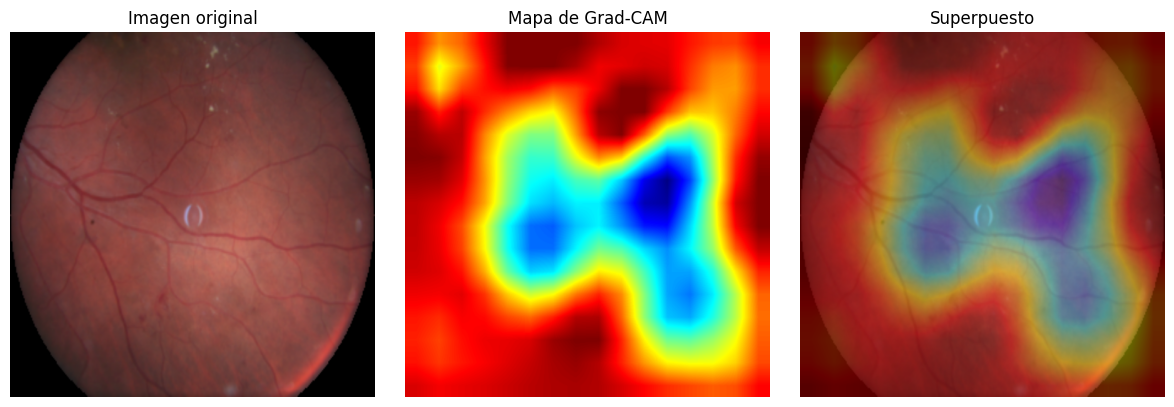
\includegraphics[scale=0.45]{doc_images/gram1.png}
		\caption{Visualización Grad-CAM de una imagen correctamente clasificada como de mala calidad.} 
		\label{fig:gram1}
	\end{figure}
\end{center}

En la Figura \ref{fig:gram1} se presenta un ejemplo correctamente clasificado como imagen de mala calidad, donde el modelo focaliza su atención en un reflejo generado por la cámara y en la ausencia de estructuras clave como el disco óptico y la mácula, indicadores consistentes con la etiqueta real.

\begin{center}
	\begin{figure}[H]
		\centering
		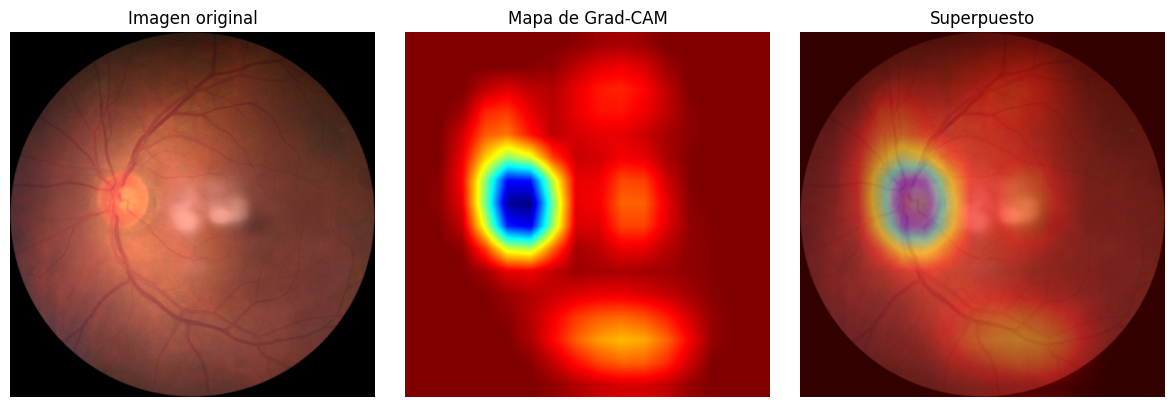
\includegraphics[scale=0.45]{doc_images/gram2.png}
		\caption{Visualización Grad-CAM de una imagen mal clasificada: el modelo la predice como de buena calidad, aunque está etiquetada como mala.} 
		\label{fig:gram2}
	\end{figure}
\end{center}

La Figura \ref{fig:gram2} muestra un caso mal clasificado, en el que la imagen es efectivamente de mala calidad, pero el modelo la predice como buena. Se observa que la atención se concentra en la mácula y los vasos sanguíneos visibles, lo que sugiere que el modelo prioriza la detección de ciertas estructuras anatómicas para inferir la calidad, incluso si existen artefactos en otras zonas.


\begin{center}
	\begin{figure}[H]
		\centering
		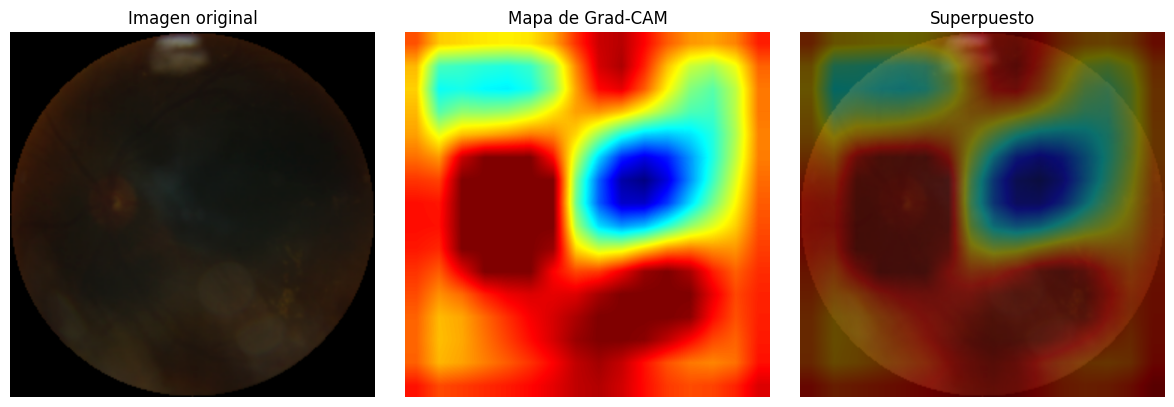
\includegraphics[scale=0.45]{doc_images/gram3.png}
		\caption{Visualización Grad-CAM de una imagen etiquetada como de buena calidad pero clasificada como de mala.} 
		\label{fig:gram3}
	\end{figure}
\end{center}

Finalmente, en la Figura \ref{fig:gram3} se presenta una imagen etiquetada como de buena calidad, pero clasificada por el modelo como de mala calidad. El modelo parece haber identificado correctamente que la imagen está oscura y contiene varios artefactos. Esto sugiere que, en algunos casos, la decisión del modelo podría incluso ser más coherente con criterios objetivos de calidad que la etiqueta asignada manualmente.

\section{Implementación y entorno de desarrollo}
La implementación del modelo se realizó en Python (3.10.15), utilizando el framework PyTorch (versión 2.5.0) para la definición, entrenamiento y evaluación de redes neuronales convolucionales. Se emplearon además las siguientes librerías complementarias: Torchvision (0.20.0) para la carga y transformación de imágenes, OpenCV (4.10.0) y PIL (10.4.0) para el procesamiento de imágenes, scikit-learn (1.5.2) para el cálculo de métricas de desempeño, NumPy (2.0.1) para operaciones matriciales, Matplotlib (3.9.2) para visualización de resultados, Pandas (2.2.3) para la manipulación de datos tabulares. El desarrollo se llevó a cabo en el entorno Visual Studio Code sobre un sistema operativo Windows 11 Pro. La ejecución del modelo se aceleró mediante una GPU NVIDIA GeForce RTX 4090 con 16 GB de memoria dedicada, utilizando CUDA versión 12.7 y el controlador NVIDIA 566.03. El equipo cuenta además con un procesador Intel Core (Intel64 Family 6 Model 186 Stepping 2) y 64 GB de memoria RAM. Todos los experimentos se realizaron en modo de usuario (WDDM), permitiendo la ejecución simultánea de procesos gráficos y de cómputo sin interferencias significativas en el rendimiento del modelo.

El código completo del modelo, así como los scripts utilizados para el entrenamiento, la evaluación y la generación de visualizaciones, se encuentra disponible en el siguiente repositorio: \url{https://github.com/gabimoran/MiM.git}

	\chapter{Clasificación con modelos multimodales (GPT-4o)}

En los últimos años, los grandes modelos de lenguaje multimodal han experimentado un crecimiento acelerado, tanto en capacidades como en su adopción en diversas áreas. Estos modelos tienen la habilidad de comprender, procesar y generar contenido integrando simultáneamente múltiples modalidades de datos, tales como texto, imágenes, audio, video y datos tabulares.

En particular, GPT-4o, el modelo multimodal más reciente desarrollado por OpenAI\footnote{GPT-4o lanzado el 13 de mayo de 2024. \url{https://openai.com/index/hello-gpt-4o/}}, es capaz de recibir entradas combinadas de texto e imágenes, y generar respuestas textuales coherentes y contextualizadas. Su diseño permite realizar tareas complejas mediante instrucciones en lenguaje natural, destacándose por su facilidad de uso, ya que está disponible mediante una interfaz de programación (API) que no requiere entrenamiento adicional específico por parte del usuario \parencites{openai2024gpt4o,shahriar2024gpt4o}. Estas características hacen que GPT-4o sea especialmente atractivo para aplicaciones prácticas en múltiples dominios donde se requiere una rápida adaptación y facilidad operativa, incluso por usuarios sin conocimientos técnicos profundos en aprendizaje automático.

El objetivo de esta sección es evaluar experimentalmente el rendimiento de dos estrategias de consulta a GPT-4o en comparación con nuestro modelo especializado (ResNet-18 fine-tuned). Aprovechando la facilidad de uso y la capacidad de generalización de los grandes modelos multimodales, basta con enviar cada imagen —o, en el segundo enfoque, pequeños ejemplos de referencia— al endpoint de OpenAI para obtener una predicción directa (“buena calidad” vs. “mala calidad”), sin necesidad de diseñar, entrenar o ajustar manualmente una red. De este modo, podemos medir qué precisión y utilidad práctica ofrece GPT-4o como alternativa de clasificación en el contexto del análisis automático de calidad de imágenes de fondo de ojo, y compararlo objetivamente con la solución basada en ResNet-18.

El proceso de consulta a GPT-4o se enmarca dentro del paradigma de \textit{in-context learning}, según el cual el modelo aprende a resolver una tarea a partir de la información (instrucciones y ejemplos) que se le proporciona directamente en el prompt, sin necesidad de un entrenamiento extenso o ajuste fino (fine-tuning) específico para cada tarea \parencites{chen2023gpt4vision}. De este modo, podemos distinguir dos modalidades principales:

\begin{itemize}
	\item \textbf{Zero-shot:} el modelo recibe únicamente una descripción de la tarea, sin ejemplos de referencia.
	\item \textbf{Few-shot:} además de la descripción, se incluyen unos pocos ejemplos etiquetados que sirven como contraste para guiar la predicción.
\end{itemize}

La muestra utilizada estuvo compuesta por 10.000 imágenes, con una proporción aproximada del 96\% correspondientes a imágenes de buena calidad (0) y 4\% de mala calidad (1), respetando la distribución real del conjunto de testeo.

\section{Zero-shot}
Se le presentó al modelo una imagen por vez, junto con un prompt en inglés que indicaba explícitamente la tarea:

\begin{table}[H]
	\renewcommand{\arraystretch}{3}
	\resizebox{\textwidth}{!}{
		\begin{tabular}{ ||l||  }
			\hline
			\makecell[l]{\textbf{Prompt:}\\
				\hspace*{3em}Classify the image as either 'Good quality' or 'Poor quality'. \\
				\hspace*{3em}Only respond with one of those two options.} \\
			\hline
		\end{tabular}
		}
	\caption{Prompt usado para clasificación zero-shot con GPT-4o.}
	\label{tab:promtZeroShot}
\end{table}

\begin{table}[H]
	\centering
	\renewcommand{\arraystretch}{1.5}
	\begin{tabular}{ ||ccccc||  }
		\hline
		\textbf{Clase} & \textbf{Precision} & \textbf{Recall} & \textbf{f1-score} & \textbf{Support} \\
		\hline
		0 (Buena) & 0.98 & 0.63 & 0.77 & 9,573 \\
		\hline
		1 (Mala) & 0.08 & 0.69 & 0.14 & 427 \\
		\hline
		Accuracy &  &  & 0.63 & 10,000 \\
		\hline
		Macro promedio & 0.53 & 0.66 & 0.45 & 10,000 \\
		\hline
		Promedio ponderado & 0.94 & 0.63 & 0.74 & 10,000 \\
		\hline
	\end{tabular}
	\caption{Classification report del modelo GPT-4o, modalidad zero-shot, evaluado sobre la muestra de test.}
	\label{tab:evaluacionZeroShot}
\end{table}

\begin{table}[H]
	\centering
	\renewcommand{\arraystretch}{1.5}
	\begin{tabular}{ ||lrr||  }
		\hline
		& \textbf{Predicho: Buena (0)} & \textbf{Predicho: Mala (1)} \\
		\hline
		Real: Buena (0) & 6,025 & 3,548 \\
		\hline
		Real: Mala (1) & 132  & 295 \\
		\hline
	\end{tabular}
	\caption{Matriz de confusión del modelo GPT-4o, modalidad zero-shot, evaluado sobre la muestra de test.}
	\label{tab:matrizZeroShot}
\end{table}

Se observa que, aunque el modelo logra identificar una parte significativa de las imágenes de mala calidad (recall 69\%), su precisión sobre esa clase es extremadamente baja (8\%), lo que indica una alta tasa de falsos positivos.

El F1-score para la clase 1 fue apenas 14\%, lo cual revela una clara dificultad del modelo en distinguir correctamente las imágenes de mala calidad en ausencia de contexto visual. En contraste, el desempeño sobre la clase mayoritaria (buena calidad) fue más equilibrado, con un F1-score de 77\%.

\subsection{Evaluación cualitativa con explicaciones generadas por GPT-4o modalidad zero shot}
Con el objetivo de analizar el razonamiento del modelo multimodal, se tomaron las tres imágenes (\ref{fig:gram1}, \ref{fig:gram2}, \ref{fig:gram3}) previamente utilizadas para generar mapas de activación Grad-CAM con la red ResNet-18 ajustada. Estas imágenes fueron procesadas individualmente por GPT-4o, esta vez utilizando un prompt extendido que solicitaba una predicción acompañada de una explicación detallada:

\begin{table}[H]
	\renewcommand{\arraystretch}{5}
	\resizebox{\textwidth}{!}{
		\begin{tabular}{ ||l||  }
			\hline
			\makecell[l]{\textbf{Prompt:}\\
				\hspace*{3em}Instruction: classify the image as either 'Good quality' or 'Poor quality'.\\
				\hspace*{3em}Please first output one line with the predicted label.\\
				\hspace*{3em}In the next line, provide a comprehensive explanation of your classification.\\
				\hspace*{3em}Consider image quality aspects such as sharpness, brightness, contrast, and the \\
				\hspace*{3em}visibility of anatomical structures like the optic disc, macula, and vessels.}\\
			\hline
		\end{tabular}
	}
	\caption{Prompt usado para clasificación zero-shot con GPT-4o.}
	\label{tab:promtZeroShotExplicacion}
\end{table}

A continuación, se presentan los resultado:

\begin{enumerate}
	\item \textbf{Imagen:} \ref{fig:gram1}:
	\begin{itemize}
		\item \textbf{Label real:} Mala calidad (1).
		\item \textbf{Predicción ResNet:} Mala calidad (1).
		\item \textbf{Predicción GPT-4o Zero-shot:} Good quality (0).
		\item \textbf{Explicación GPT-4o Zero-shot:} The image exhibits clear visibility of key anatomical structures such as the optic disc, macula, and blood vessels. The sharpness is adequate, with distinct and well-defined vessel outlines. The brightness and contrast levels are balanced, helping to highlight important details and ensuring that the overall view is not obscured by excessive dark or bright areas.
	\end{itemize}
	\item \textbf{Imagen:} \ref{fig:gram2}:
		\begin{itemize}
		\item \textbf{Label real:} Mala calidad (1).
		\item \textbf{Predicción ResNet:} Buena calidad (0).
		\item \textbf{Predicción GPT-4o Zero-shot:} Good quality (0).
		\item \textbf{Explicación GPT-4o Zero-shot:} The image is classified as 'Good quality' because it demonstrates clear visibility of essential anatomical structures such as the optic disc, macula, and vessels. The sharpness is sufficient, with distinct outlines of the retinal features. The brightness and contrast are well-balanced, providing a clear view of the different elements within the eye.
	\end{itemize}
	\item \textbf{Imagen:} \ref{fig:gram3}:
	\begin{itemize}
		\item \textbf{Label real:} Buena calidad (0).
		\item \textbf{Predicción ResNet:} Mala calidad (1).
		\item \textbf{Predicción GPT-4o Zero-shot:} Poor quality (1).
		\item \textbf{Explicación GPT-4o Zero-shot:} The image is classified as poor quality because it lacks sufficient brightness and sharpness, making it difficult to discern key anatomical structures such as the optic disc, macula, and blood vessels. The overall image is dark, and there is a lack of contrast, which further obscures important details necessary for a clear analysis.
	\end{itemize}
\end{enumerate}

En los tres casos analizados, el modelo GPT-4o en modalidad zero-shot demostró prestar atención a aspectos similares a los considerados por el modelo ResNet-18 ajustado, tales como la nitidez de las estructuras anatómicas, el contraste y la iluminación general de la imagen. Sin embargo, en el primer ejemplo, GPT-4o no logró identificar un artefacto crítico, un reflejo de la cámara, que determinaba la calidad de la imagen. Este defecto fue correctamente detectado por la red ResNet fine-tuned, lo que sugiere que, además de no estar específicamente entrenado en el dominio, el modelo puede verse limitado por la formulación del prompt. Es posible que la omisión de instrucciones explícitas sobre la detección de artefactos haya contribuido a esta predicción errónea, lo que refuerza la importancia del diseño del prompt al evaluar modelos multimodales en contextos clínicos. Esto motivó una segunda prueba, en la que se reformuló el prompt incluyendo de manera explícita la necesidad de considerar artefactos técnicos como reflejos y desenfoques.

\begin{table}[H]
	\renewcommand{\arraystretch}{5}
	\resizebox{\textwidth}{!}{
		\begin{tabular}{ ||l||  }
			\hline
			\makecell[l]{\textbf{Prompt:}\\
				\hspace*{3em}Instruction: classify the image as either 'Good quality' or 'Poor quality'.\\
				\hspace*{3em}Please first output one line with the predicted label.\\
				\hspace*{3em}In the next line, provide a comprehensive explanation of your classification.\\
				\hspace*{3em}Consider image quality aspects such as sharpness, brightness, contrast, and the \\
				\hspace*{3em}visibility of anatomical structures like the optic disc, macula, and vessels. \\
				\hspace*{3em}Also consider the presence of image artifacts such as glare, reflections, \\
				\hspace*{3em}vignetting, blurred edges, or any other technical issues that may impair diagnostic usability.}\\
			\hline
		\end{tabular}
	}
	\caption{Prompt usado para clasificación e interpretación zero-shot con GPT-4o, incluyendo en el prompt la necesidad de considerar artefactos.}
	\label{tab:promtZeroShotExplicacionArtefactos}
\end{table}

A continuación, se presentan los resultado:

\begin{enumerate}
	\item \textbf{Imagen:} \ref{fig:gram1}:
	\begin{itemize}
		\item \textbf{Label real:} Mala calidad (1).
		\item \textbf{Predicción ResNet:} Mala calidad (1).
		\item \textbf{Predicción GPT-4o Zero-shot:} Good quality (0).
		\item \textbf{Predicción GPT-4o Zero-shot (menciona artefactos en el prompt):} Poor quality (1).
		\item \textbf{Explicación GPT-4o Zero-shot (menciona artefactos en el prompt):} The image is classified as poor quality due to several factors: 
		1. \textbf{Sharpness}: The image appears blurry, and the details of anatomical structures like the optic disc and macula may not be clearly visible.
		2. \textbf{Brightness and Contrast}: The image seems to lack the proper balance of brightness and contrast, making it difficult to distinguish between different structures.
		3. \textbf{Artifacts}: There is a noticeable \textcolor{red}{glare at the center}, which could obscure important diagnostic features. Additionally, there is some vignetting around the edges, further diminishing image usability.
		4. \textbf{Visibility of Structures}: Given the blurriness and glare, it may be challenging to accurately assess the vessels and other critical areas for diagnostic purposes. Overall, these issues significantly impair the diagnostic usability of the image.
	\end{itemize}
	\item \textbf{Imagen:} \ref{fig:gram2}:
	\begin{itemize}
		\item \textbf{Label real:} Mala calidad (1).
		\item \textbf{Predicción ResNet:} Buena calidad (0).
		\item \textbf{Predicción GPT-4o Zero-shot:} Good quality (0).
		\item \textbf{Predicción GPT-4o Zero-shot (menciona artefactos en el prompt):} Poor quality (1).
		\item \textbf{Explicación GPT-4o Zero-shot (menciona artefactos en el prompt):} The image suffers from significant issues that impair its diagnostic usability. There is a prominent blurred area in the center, which obscures critical anatomical structures like the macula and part of the retinal vessels. Additionally, there is glare or reflections that further obscure the visibility. Although the optic disc is somewhat visible, the overall sharpness and contrast of the image are inadequate, with a lack of clarity and definition in the vessels and surrounding areas. These artifacts significantly impact the image quality, making it unsuitable for diagnostic purposes.
	\end{itemize}
	\item \textbf{Imagen:} \ref{fig:gram3}:
	\begin{itemize}
		\item \textbf{Label real:} Buena calidad (0).
		\item \textbf{Predicción ResNet:} Mala calidad (1).
		\item \textbf{Predicción GPT-4o Zero-shot:} Poor quality (1).
		\item \textbf{Predicción GPT-4o Zero-shot (menciona artefactos en el prompt):} Poor quality (1).
		\item \textbf{Explicación GPT-4o Zero-shot (menciona artefactos en el prompt):} The image appears to be of poor quality due to several factors. It's dark, lacking sufficient brightness and contrast to clearly distinguish anatomical structures like the optic disc, macula, and blood vessels. These key features are not clearly visible, which impacts its diagnostic usability. There are noticeable artifacts such as glare and blurred areas that further reduce the overall image quality. These issues collectively impair the clarity and diagnostic value of the retinal image.
	\end{itemize}
\end{enumerate}

Como resultado, GPT-4o no solo cambió sus predicciones, clasificando las tres imágenes como de mala calidad, sino que también ofreció explicaciones más detalladas en las que mencionó los artefactos detectados.

Sin embargo, este comportamiento plantea interrogantes. Por un lado, el modelo parece volverse más sensible a la presencia de cualquier elemento mencionado en el prompt, sin necesariamente evaluar si dicho defecto compromete efectivamente la utilidad clínica de la imagen. Por otro, se observa hasta qué punto la formulación del prompt condiciona el tipo de respuesta: lejos de ser una herramienta objetiva, GPT-4o adapta su criterio según las instrucciones, lo que implica un riesgo de sesgo si el diseño del prompt no está cuidadosamente calibrado. Por eso, aunque la capacidad del modelo para detectar artefactos mejora, es necesario comprobar si esas decisiones realmente ayudan al diagnóstico en la práctica. No alcanza con que el modelo diga algo razonable, hace falta validar que sus respuestas sean útiles y correctas en el contexto clínico donde se piensa aplicar.



\section{Few-shot}
En este caso, a diferencia del escenario zero-shot, se le presentaron al modelo tres imágenes de forma simultánea, combinadas en una sola figura. Las imágenes de referencia fueron extraídas del conjunto de entrenamiento, mientras la tercera imágen, sin etiqueta visible, corresponde al conjunto de test.

\begin{center}
	\begin{figure}[H]
		\centering
		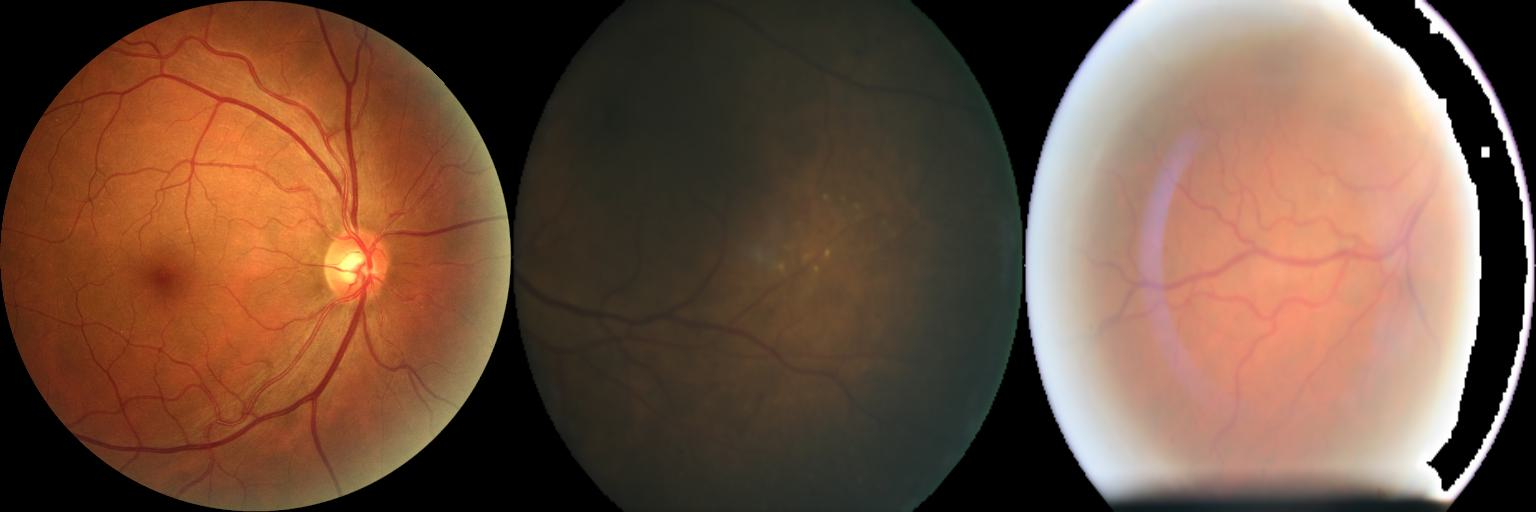
\includegraphics[scale=0.25]{doc_images/composite_test.jpg}
		\caption{Ejemplo de imagen compuesta utilizada en el esquema few-shot: buena calidad, mala calidad y muestra a clasificar (de izquierda a derecha).} 
		\label{fig:composite_test}
	\end{figure}
\end{center}

\begin{table}[H]
	\renewcommand{\arraystretch}{5}
	\resizebox{\textwidth}{!}{
		\begin{tabular}{ ||l||  }
			\hline
			\makecell[l]{\textbf{Prompt:}\\
				\hspace*{3em}Instruction: classify the images into two classes: 'Good quality', 'Poor quality'.\\
				\hspace*{3em}Example: the label of the above images:\\
				\hspace*{3em}Image 1: Good quality\\
				\hspace*{3em}Image 2: Poor quality\\
				\hspace*{3em}Please output one line with the predicted label for Image 3.}\\
			\hline
		\end{tabular}
	}
	\caption{Prompt usado para clasificación few-shot con GPT-4o.}
	\label{tab:promtFewShot}
\end{table}

Este diseño le permite al modelo inferir las características que definen cada clase a partir de ejemplos visuales, antes de emitir su predicción sobre la tercera imagen. Todas las imágenes de evaluación fueron clasificadas individualmente bajo esta modalidad, manteniendo constantes las dos imágenes de referencia (una buena y una mala) en todos los casos.

Dado que GPT-4o no conserva memoria entre solicitudes individuales, cada predicción se realiza de manera independiente, sin influencias del desbalance de clases presente en el conjunto evaluado. Esto implica que el modelo no ajusta su criterio de decisión en función de la frecuencia relativa de cada clase, como sí podría ocurrir en modelos entrenados explícitamente sobre el dominio.

\begin{table}[H]
	\centering
	\renewcommand{\arraystretch}{1.5}
	\begin{tabular}{ ||ccccc||  }
		\hline
		\textbf{Clase} & \textbf{Precision} & \textbf{Recall} & \textbf{f1-score} & \textbf{Support} \\
		\hline
		0 (Buena) & 0.98 & 0.51 & 0.67 & 9,573 \\
		\hline
		1 (Mala) & 0.07 & 0.78 & 0.12 & 427 \\
		\hline
		Accuracy &  &  & 0.52 & 10,000 \\
		\hline
		Macro promedio & 0.52 & 0.65 & 0.40 & 10,000 \\
		\hline
		Promedio ponderado & 0.94 & 0.52 & 0.65 & 10,000 \\
		\hline
	\end{tabular}
	\caption{Classification report del modelo GPT-4o, modalidad few-shot, evaluado sobre la muestra de test.}
	\label{tab:evaluacionFewShot}
\end{table}

\begin{table}[H]
	\centering
	\renewcommand{\arraystretch}{1.5}
	\begin{tabular}{ ||lrr||  }
		\hline
		& \textbf{Predicho: Buena (0)} & \textbf{Predicho: Mala (1)} \\
		\hline
		Real: Buena (0) & 4,895 & 4,678 \\
		\hline
		Real: Mala (1) & 93  & 334 \\
		\hline
	\end{tabular}
	\caption{Matriz de confusión del modelo GPT-4o, modalidad few-shot, evaluado sobre la muestra de test.}
	\label{tab:matrizFewShot}
\end{table}

A pesar de agregar más información visual al contexto, el desempeño general fue inferior al observado en la modalidad zero-shot, con un accuracy global de apenas 52\%. En particular, el modelo mostró una alta sensibilidad para la clase minoritaria (recall 78\% para imágenes de mala calidad), pero una muy baja precisión (7\%), lo que implica una gran cantidad de falsos positivos. El F1-score para la clase 1 fue de 12\%, confirmando la dificultad del modelo para distinguir de manera precisa las imágenes de baja calidad, incluso cuando se le ofrecen ejemplos visuales. Por otro lado, el rendimiento sobre la clase mayoritaria también se vio afectado: el recall descendió al 51\%, con un F1-score de 67\%.

\subsection{Evaluación cualitativa con explicaciones generadas por GPT-4o modalidad few-shot}
Repetimos el experimento realizado para la modalidad zero-shot sobre las tres imágenes (\ref{fig:gram1}, \ref{fig:gram2}, \ref{fig:gram3}) previamente utilizadas para generar mapas de activación Grad-CAM con la red ResNet-18 ajustada. Estas imágenes fueron procesadas individualmente por GPT-4o, esta vez utilizando un prompt extendido que solicitaba una predicción acompañada de una explicación detallada:

\begin{table}[H]
	\renewcommand{\arraystretch}{5}
	\resizebox{\textwidth}{!}{
		\begin{tabular}{ ||l||  }
			\hline
			\makecell[l]{\textbf{Prompt:}\\
				\hspace*{3em}Instruction: classify the images into two classes: 'Good quality', 'Poor quality'.\\
				\hspace*{3em}Example: the label of the above images:\\
				\hspace*{3em}Image 1: Good quality\\
				\hspace*{3em}Image 2: Poor quality \\
				\hspace*{3em}Please output one line with the predicted label for Image 3.\\
				\hspace*{3em}In the next line, provide a comprehensive explanation of your classification.\\
				\hspace*{3em}Consider image quality aspects such as sharpness, brightness, contrast, and the\\
				\hspace*{3em}visibility of anatomical structures like the optic disc, macula, and vessels.}\\
			\hline
		\end{tabular}
	}
	\caption{Prompt usado para clasificación e interpretación few-shot con GPT-4o.}
	\label{tab:promtFewShotExplicacion}
\end{table}

A continuación, se presentan los resultado:

\begin{enumerate}
	\item \textbf{Imagen:} \ref{fig:gram1}:
	\begin{itemize}
		\item \textbf{Label real:} Mala calidad (1).
		\item \textbf{Predicción ResNet:} Mala calidad (1).
		\item \textbf{Predicción GPT-4o Few-shot:} Poor quality (1).
		\item \textbf{Explicación GPT-4o Few-shot:} The third image exhibits characteristics of poor quality. It appears to have lower brightness and contrast compared to a good quality image. The anatomical structures such as the optic disc, macula, and blood vessels are not as clearly visible or well-defined. These features make it difficult to assess the image for medical or diagnostic purposes, categorizing it as poor quality.
	\end{itemize}
	\item \textbf{Imagen:} \ref{fig:gram2}:
	\begin{itemize}
		\item \textbf{Label real:} Mala calidad (1).
		\item \textbf{Predicción ResNet:} Buena calidad (0).
		\item \textbf{Predicción GPT-4o Few-shot:} Poor quality (1)).
		\item \textbf{Explicación GPT-4o Few-shot:} The image exhibits low brightness and contrast, making it difficult to clearly distinguish the anatomical structures like the optic disc, macula, and vessels. The sharpness is not sufficient to provide a clear and detailed view, which is crucial for a good quality classification.
	\end{itemize}
	\item \textbf{Imagen:} \ref{fig:gram3}:
	\begin{itemize}
		\item \textbf{Label real:} Buena calidad (0).
		\item \textbf{Predicción ResNet:} Mala calidad (1).
		\item \textbf{Predicción GPT-4o Few-shot:} Poor quality (1).
		\item \textbf{Explicación GPT-4o Few-shot:} The third image exhibits several signs of poor quality. It lacks adequate sharpness, making the anatomical structures like the optic disc, macula, and retinal vessels difficult to discern. Additionally, the brightness and contrast are insufficient, resulting in a dim and washed-out appearance that further obscures important details necessary for proper examination and analysis. This lack of clarity and definition categorizes it as poor quality.
	\end{itemize}
\end{enumerate}

En esta configuración, GPT-4o clasificó las tres imágenes como de mala calidad y las explicaciones ofrecidas por el modelo sugieren que, GPT-4o tiende a comparar directamente la imagen a clasificar con las imágenes de ejemplo provistas, en lugar de aplicar un criterio clínico general. Por ejemplo, se observa que menciona diferencias relativas en brillo o contraste respecto a la imagen de referencia de buena calidad, lo que sugiere una evaluación basada en comparación visual directa más que en estándares absolutos. Esto introduce nuevas variables que impactan en la predicción: la selección específica de las imágenes de ejemplo y la cantidad de ejemplos utilizados. A diferencia de los modelos entrenables, aquí no está claro cuánto peso tiene el contenido visual de las imágenes versus el texto del prompt. Esta falta de transparencia complica la interpretación del razonamiento del modelo y refuerza la necesidad de calibrar cuidadosamente tanto el prompt como la selección de ejemplos para evitar sesgos en la clasificación.


	
	\chapter*{Resultados finales}
\addcontentsline{toc}{chapter}{Resultados finales}

Como se observa en el cuadro \ref{tab:resumen_resultados}, el modelo ResNet-18 fine-tuned presentó el mejor desempeño general en la tarea de clasificación de calidad de imágenes retinianas, alcanzando una exactitud del 97\% y un F1-score del 0.58 para la clase minoritaria (mala calidad). En contraste, las modalidades basadas en GPT-4o mostraron desempeños más limitados, particularmente en términos de precisión para la clase 1, con valores cercanos al 7-8\%. No obstante, ambas configuraciones de GPT-4o lograron recalls relativamente altos (69\% en modalidad zero-shot y 78\% en few-shot), lo que indica que el modelo tiende a identificar correctamente muchas imágenes de mala calidad, pero al costo de una gran cantidad de falsos positivos. Esta diferencia sugiere que, mientras la ResNet-18 ajustada toma decisiones más conservadoras pero precisas (dice que una imagen es mala cuando está muy segura, aunque eso implique no detectar todas las malas), GPT-4o tiene un umbral más permisivo: tiende a marcar muchas imágenes como malas, aunque no todas lo sean realmente. Esta conducta puede estar influenciada por el lenguaje del prompt o, en la modalidad few-shot, por la comparación visual directa con los ejemplos proporcionados. Estas observaciones resaltan tanto el potencial como las limitaciones actuales de los modelos multimodales de propósito general aplicados a tareas clínicas específicas.

\begin{table}[H]
	\centering
	\renewcommand{\arraystretch}{1.6}
	\resizebox{\textwidth}{!}{
		\begin{tabular}{|l|c|c|c|c|c|}
			\hline
			\textbf{Modelo / Modalidad} & \textbf{Accuracy} & \textbf{Precisión (clase 1)} & \textbf{Recall (clase 1)} & \textbf{F1-score (clase 1)} & \textbf{Entrada} \\
			\hline
			ResNet-18 fine-tuned &  0.97 & 0.73 & 0.49 & 0.58 & Imagen sola \\
			
			GPT-4o zero-shot (prompt simple) & 0.63 & 0.08 & 0.69 & 0.14 & Imagen + prompt \\
			GPT-4o few-shot (ICL2) & 0.52 & 0.07 & 0.78 & 0.12 & Imagen compuesta (3) + prompt \\
			\hline
		\end{tabular}
	}
	\caption{Resumen de métricas principales para cada modelo y configuración evaluada. Las métricas se centran en la clase minoritaria (clase 1 = mala calidad).}
	\label{tab:resumen_resultados}
\end{table}

	\chapter*{Conclusiones}
\addcontentsline{toc}{chapter}{Conclusiones}

Este trabajo se propuso comparar dos enfoques diferentes para resolver una tarea clínica sensible como es la evaluación de la calidad de imágenes retinianas: un modelo entrenado específicamente (ResNet-18 fine-tuned) y un modelo multimodal de propósito general (GPT-4o) utilizado sin entrenamiento adicional, bajo modalidades zero-shot y few-shot.

Los resultados muestran que, en términos cuantitativos, el modelo entrenado ofreció un desempeño significativamente superior, tanto en precisión como en estabilidad. GPT-4o, en cambio, demostró una sensibilidad alta pero con una gran cantidad de falsos positivos, lo cual compromete su confiabilidad como herramienta autónoma en un contexto clínico.

Desde el punto de vista práctico, los modelos multimodales presentan ventajas importantes, especialmente en modalidad zero-shot, donde no requieren recolección ni etiquetado de datos ni conocimientos técnicos avanzados para su uso. En few-shot, si bien se requiere una selección previa de ejemplos etiquetados, el volumen de datos necesarios sigue siendo considerablemente menor en comparación con un proceso completo de entrenamiento supervisado. Sin embargo, este menor esfuerzo técnico inicial no elimina la necesidad de conocimiento experto: al momento de diseñar el prompt o elegir las imágenes de ejemplo, se hace evidente que el desempeño del modelo depende en gran medida de la claridad y relevancia clínica de estas decisiones. Aún así, los modelos multimodales siguen representando herramientas de bajo esfuerzo y rápida implementación. No obstante, este mismo grado de flexibilidad puede volverse difícil de controlar: el diseño del prompt y la selección de ejemplos demostraron tener un impacto directo en la predicción, lo cual reintroduce un sesgo que los modelos de redes neuronales intentan minimizar: el sesgo del investigador. En este sentido, el prompt engineering funciona casi como una nueva forma de "ingeniería de features".

También debe considerarse el aspecto económico. Si bien el costo de uso de GPT-4o fue accesible en esta tesis (aproximadamente 17 USD para procesar 10.000 imágenes en modalidad few-shot), sigue siendo un modelo ofrecido como servicio. Cada clasificación implica una llamada a la API, cuyo costo varía según el tamaño del input y la longitud de la respuesta. En contraste, los modelos como ResNet-18 pueden descargarse gratuitamente y ejecutarse localmente, aunque el fine-tuning requiere recursos de cómputo cuyo costo, aunque presente, es más predecible y bajo control del desarrollador.

Además, el uso de modelos ofrecidos como servicio, como GPT-4o, plantea desafíos para la reproducibilidad y la trazabilidad: el usuario no tiene control sobre los pesos del modelo, ni garantía de estabilidad entre versiones. Esto dificulta su integración en sistemas clínicos donde la transparencia y la validación son críticas. También deben considerarse aspectos relacionados con la seguridad, como las alucinaciones (respuestas inventadas pero plausibles), y la falta de entrenamiento específico en patologías concretas como la retinopatía diabética, lo cual limita su capacidad para ajustar su criterio al contexto clínico real.

En conclusión, si bien los modelos multimodales como GPT-4o muestran un potencial interesante como herramientas auxiliares de bajo esfuerzo, su aplicación actual en tareas clínicas automatizadas requiere precaución. Son sistemas versátiles y configurables, pero aún carecen de la robustez, precisión y trazabilidad necesarias para ser confiables en escenarios sensibles como el de la salud. Su uso futuro dependerá tanto de avances técnicos como de la capacidad para integrar estas herramientas en flujos de trabajo controlados, validados y auditables.
	\chapter*{Reflexión final}
\addcontentsline{toc}{chapter}{Reflexión final}

Este trabajo me permitió explorar no solo las capacidades técnicas de diferentes modelos, sino también las implicancias prácticas de aplicar herramientas de inteligencia artificial en un contexto clínico real y sensible. A partir de esta experiencia, considero que hay varias direcciones que podrían ser exploradas en futuras investigaciones.

Algo que me gustaría seguir profundizando es cómo lograr que modelos como GPT-4o se acerquen un poco más a criterios clínicos reales. Cambiar el prompt o las imágenes de ejemplo puede modificar totalmente lo que el modelo responde, y eso muestra tanto su potencial como sus límites. Quizás una forma de mejorar esto sea combinar este tipo de modelos con otros sistemas que tomen decisiones más controladas, como reglas clínicas o redes entrenadas específicamente para una patología.

También sería valioso desarrollar marcos de evaluación específicos para medir si estas respuestas generadas son verdaderamente útiles para profesionales de la salud, más allá de métricas numéricas. Porque a veces acierta la etiqueta, pero no necesariamente da una explicación útil o coherente desde lo clínico.

Finalmente, aunque las soluciones de bajo esfuerzo como GPT-4o son prometedoras, siguen siendo herramientas auxiliares. Por ahora, su uso en salud requiere acompañamiento, validación y responsabilidad humana. Pero con una integración cuidadosa, podrían ocupar un lugar útil en sistemas híbridos de apoyo al diagnóstico, especialmente en contextos donde los recursos son escasos y el acceso temprano a la atención puede marcar una diferencia significativa.
	
	\printbibliography[heading=bibintoc]
	
	\newpage
	\chapter*{Anexo}
\addcontentsline{toc}{chapter}{Anexo}

\begin{table*}[ht]
	\centering
	\renewcommand{\arraystretch}{1.5} % Ajusta el espaciado entre las filas
	\resizebox{\textwidth}{!}{
	\begin{tabular}{|p{4cm}|l|l|} 
		\hline
		\textbf{Método} & \textbf{Publicación} & \textbf{Descripción} \\ [0.5ex] 
		\hline
		\multirow{11}{*}{\parbox[t]{4cm}{Diseño manual de características - Estructuras del ojo}} & \parencites{lee1999automatic} & Histograma de intensidad \\ 
		\cline{2-3}
		& \parencites{lalonde2001new} & Histograma de intensidad local y magnitud de bordes \\
		\cline{2-3}
		& \parencites{bartling2009automated} & Nitidez e iluminación local \\
		\cline{2-3}
		& \parencites{davis2009vision} & Nitidez, Iluminación y textura \\
		\cline{2-3}
		& \parencites{dias2014retinal} & Color, enfoque, contraste e iluminación \\
		\cline{2-3}
		& \parencites{veiga2014quality} & Enfoque e iluminación no uniforme \\
		\cline{2-3}
		& \parencites{fasih2014retinal} & Nitidez, iluminación, textura \\
		\cline{2-3}
		& \parencites{piresdias2014retinal} & Retroproyección de histograma, enfoque, contraste, iluminación \\
		\cline{2-3}
		& \parencites{yao2016generic} & Desenfoque e iluminación no uniforme \\
		\cline{2-3}
		& \parencites{wang2016human} & Características del sistema visual humano (HVS) \\
		\cline{2-3}
		& \parencites{abdelhamid2016retinal, abdelhamid2017no} & Transformada wavelet, índice de calidad \\
		\hline
		\multirow{11}{*}{\parbox[t]{4cm}{Diseño manual de características - Estructuras del ojo}} & \parencites{usher2003density} & Densidad de vasos sanguíneos \\
		\cline{2-3}
		& \parencites{fleming2006counting} & Recuento de píxeles de vasos sanguíneos y definición del área \\
		\cline{2-3}
		& \parencites{niemeijer2006grouping} & Agrupación de píxeles en estructuras \\
		\cline{2-3}
		& \parencites{giancardo2010} & Densidad local de vasos segmentados \\
		\cline{2-3}
		& \parencites{hunter2011visibility} & Visibilidad de los vasos sanguíneos y definición de área \\
		\cline{2-3}
		& \parencites{yu2012texture} & Textura y nitidez de vasos segmentados \\
		\cline{2-3}
		& \parencites{fleming2012automated} & Regiones de relevancia y segmentación \\
		\cline{2-3}
		& \parencites{koehler2013automatic} & Textura y recuento de píxeles de vasos sanguíneos \\
		\cline{2-3}
		& \parencites{katuwal2013automatic} & Simetría de los vasos sanguíneos \\
		\cline{2-3}
		& \parencites{nugroho2014contrast} & Contraste de los vasos sanguíneos \\
		\cline{2-3}
		& \parencites{yin2014automatic} & Contraste, desenfoque y densidad de vasos sanguíneos \\
		\hline
		\multirow{3}{*}{\parbox[t]{4cm}{Diseño manual de características - Medidas de similitud y Estructuras del ojo}} & \parencites{paulus2010automated} & Segmentación estructuras, homogeneidad y contraste \\
		\cline{2-3}
		& \parencites{sevik2014retinal} & Segmentación estructuras, forma, textura e intensidad \\
		\cline{2-3}
		& \parencites{shao2018naturalness} & Propiedades de naturalidad, iluminación, segmentación del disco óptico \\
		\hline
		\multirow{7}{*}{\parbox[t]{4cm}{Extracción automática de características con CNN}} & \parencites{mahapatra2016} & Extracción de características de alto nivel \\
		\cline{2-3}
		& \parencites{costa2017eyequal} & CNN sobre parches, ponderación de respuestas \\
		\cline{2-3}
		& \parencites{yu2017image} & Fusión de características extraídas de CNN y mapas de prominencia \\
		\cline{2-3}
		& \parencites{saha2018automated} & Fine-tunning de CNN AlexNet \\
		\cline{2-3}
		& \parencites{zago2018retinal} & Fine-tunning de CNN VGG-16 \\
		\cline{2-3}
		& \parencites{fu2019evaluation} & Multiple Color-space Fusion Network \\
		\cline{2-3}
		& \parencites{shen2018multi} & Modelo multitarea. ResNet50 para detección y VGG-16 para la ubicación de las estructuras. \\
		\cline{2-3}
		& \parencites{xu2020deep} & Dualbranch SalStructIQA and Single-branch SalStructIQA \\
		\hline
	\end{tabular}
	}
	\caption{Métodos utilizados en la clasificación de imágenes de fondo de ojo para evaluar la calidad.}
	\label{tab:metodosQA}
\end{table*}


\begin{center}
	\begin{figure}[H]
		\centering
		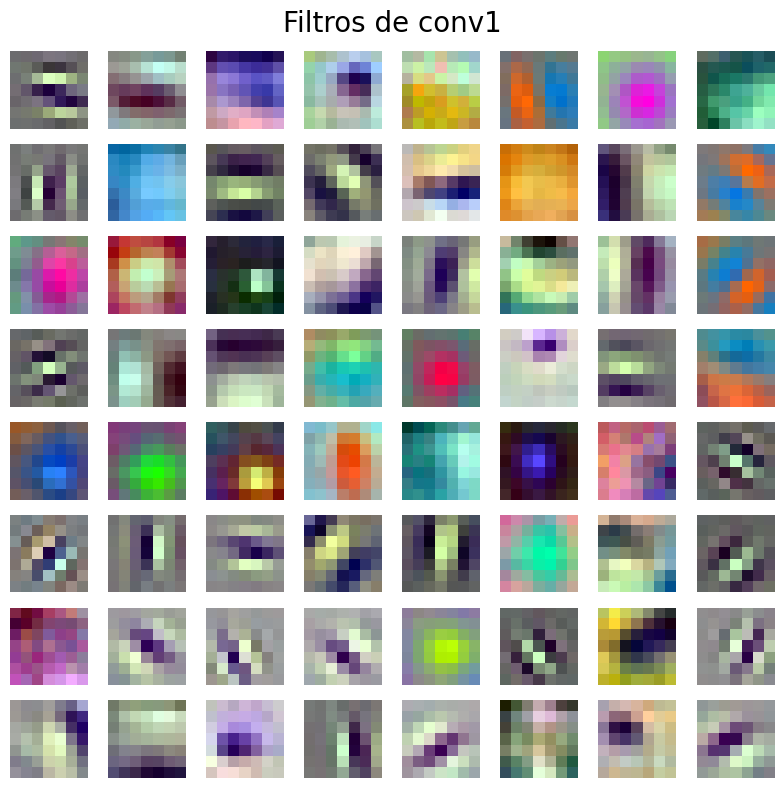
\includegraphics[scale=0.50]{doc_images/filtrosConv1.png}
		\caption{Filtros de conv1: muestra los kernels aprendidos en la primera capa, detectores de bordes y texturas en distintas frecuencias y orientaciones.} 
		\label{fig:filtrosConv1}
	\end{figure}
\end{center}

\begin{center}
	\begin{figure}[H]
		\centering
		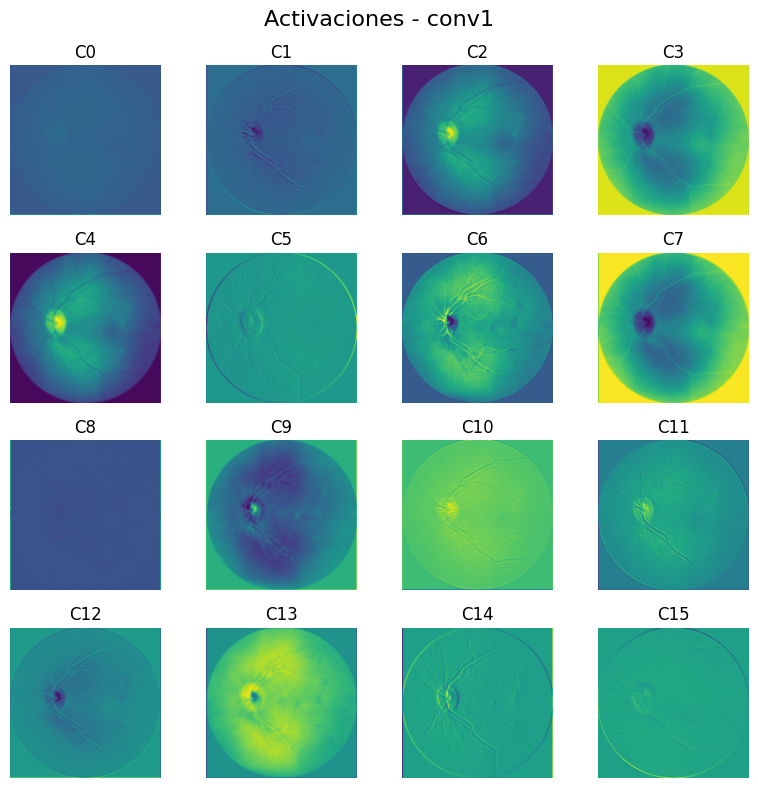
\includegraphics[scale=0.50]{doc_images/actConv1.png}
		\caption{Mapa de activación de la primera capa convolucional (conv1). Este mapa resalta características de bajo nivel, como bordes y texturas simples, tal como un detector de Gabor.} 
		\label{fig:actConv1}
	\end{figure}
\end{center}

\begin{center}
	\begin{figure}[H]
		\centering
		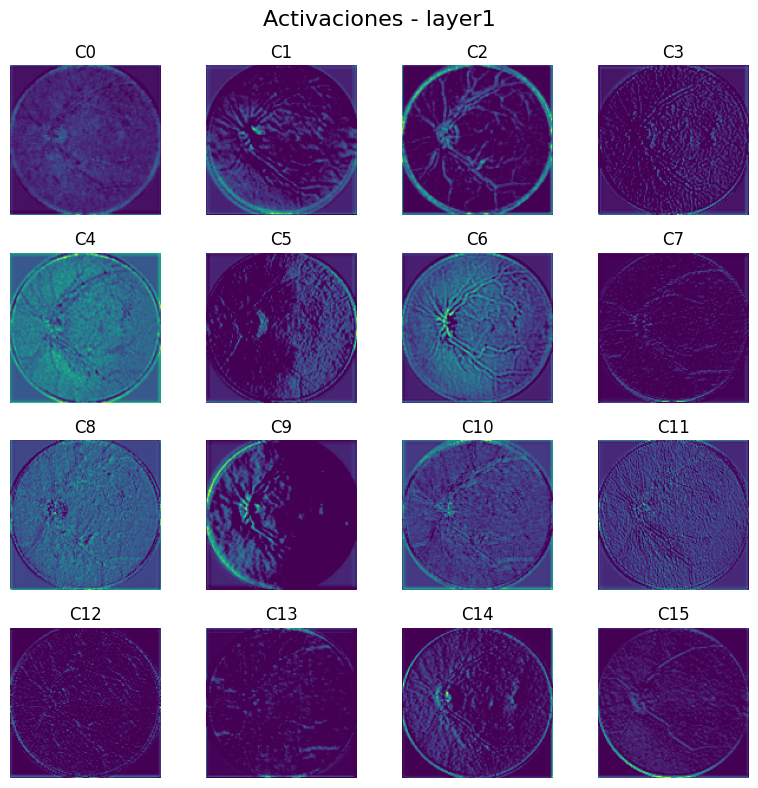
\includegraphics[scale=0.50]{doc_images/actLayer1.png}
		\caption{Mapas de activación del primer bloque residual (layer1). Estos mapas muestran la respuesta de los filtros a patrones algo más complejos, como combinaciones de bordes, esquinas y contornos.} 
		\label{fig:actLayer1}
	\end{figure}
\end{center}

\begin{center}
	\begin{figure}[H]
		\centering
		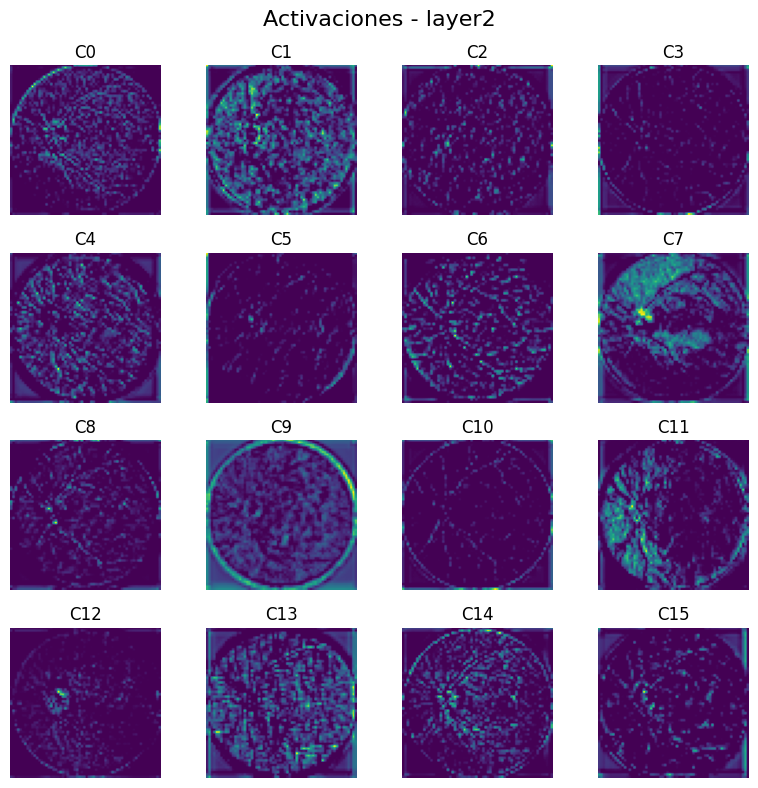
\includegraphics[scale=0.50]{doc_images/actLayer2.png}
		\caption{Mapas de activación del segundo bloque residual (layer2). Aquí ya aparecen representaciones intermedias que capturan texturas más finas y agrupaciones locales de características.} 
		\label{fig:actLayer2}
	\end{figure}
\end{center}

\begin{center}
	\begin{figure}[H]
		\centering
		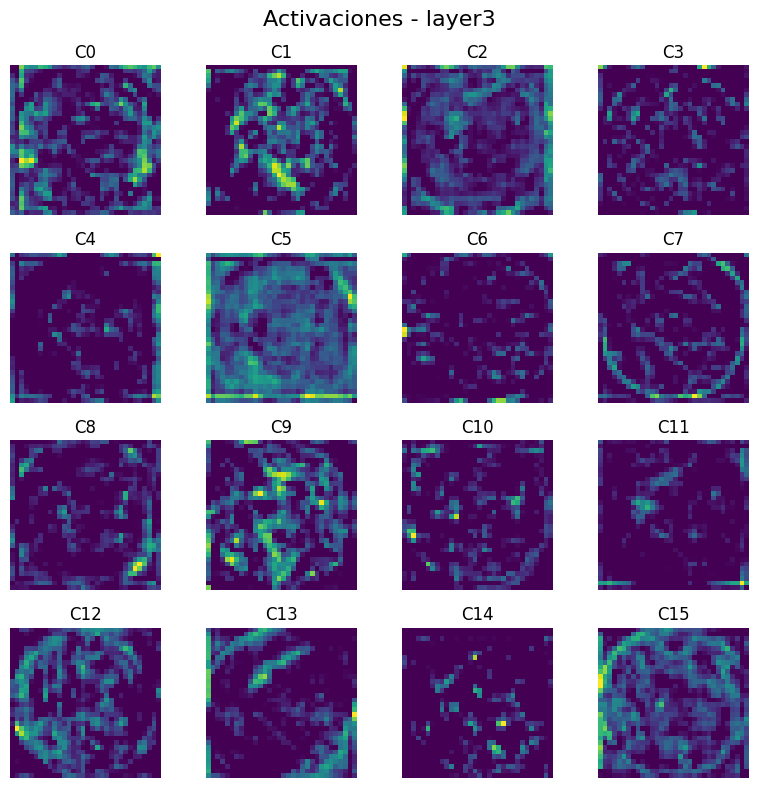
\includegraphics[scale=0.50]{doc_images/actLayer3.png}
		\caption{Mapas de activación del tercer bloque residual (layer3). Se observan patrones de nivel aún más alto, como formas globales, combinaciones de texturas, agrupación de partes, zonas específicas.} 
		\label{fig:actLayer3}
	\end{figure}
\end{center}

\begin{center}
	\begin{figure}[H]
		\centering
		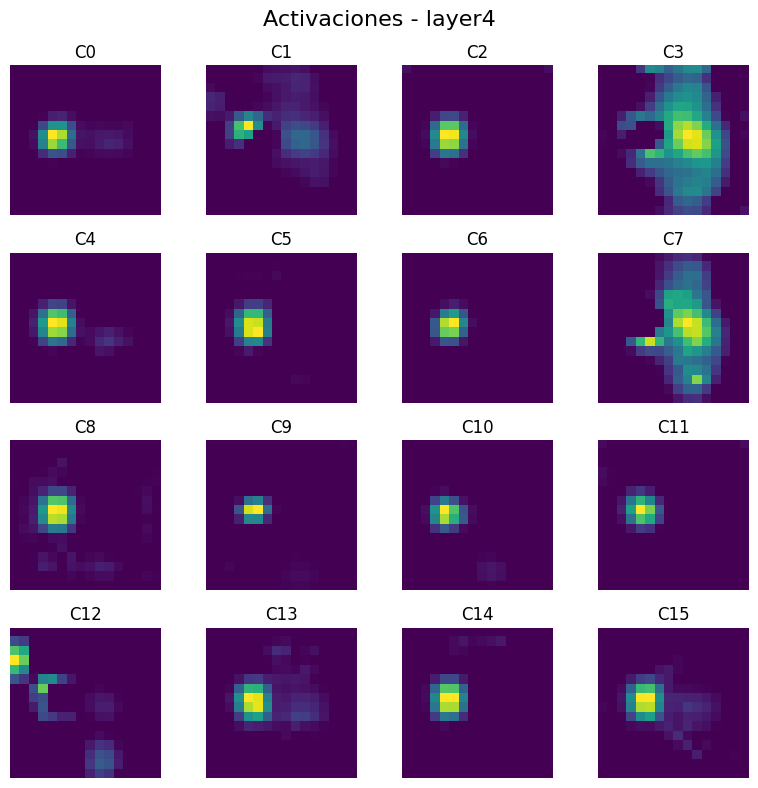
\includegraphics[scale=0.50]{doc_images/actLayer4.png}
		\caption{Mapas de activación del cuarto bloque residual (layer4). Estos mapas representan las características más abstractas aprendidas por la red, útiles para la clasificación final (ej. mácula, nervio óptico, áreas oscuras).} 
		\label{fig:actLayer4}
	\end{figure}
\end{center}
	

\end{document}